%!TEX root = ../thesis.tex
%*******************************************************************************
%*********************************** First Chapter *****************************
%*******************************************************************************

\chapter{Introduction}  %Title of the First Chapter
\label{ch:Introduction}

\ifpdf
    \graphicspath{{Chapter1/Figs/Raster/}{Chapter1/Figs/PDF/}{Chapter1/Figs/}}
\else
    \graphicspath{{Chapter1/Figs/Vector/}{Chapter1/Figs/}}
\fi


%********************************** %First Section  **************************************
\section{Introduction to piezotronics effect} %Section - 1.1 
\subsection{Development and principles of piezotronics effect}

The piezoelectric effect \index{Piezoelectric!effect} is the effect of accumulating electric charge in certain solid materials in response to applied mechanical stress, e.g. crystals, some ceramics and biological substances such as bones, DNA and various proteins \cite{skoog2017principles}. It was discovered in 1880 by brothers Pierre and Jacques Curie \cite{jacques1880development}. In 1910, German physicist W. A. Wooster published the book "A Text-Book on Crystal \index{Crystal} Physics", which described 20 natural crystals capable of producing \index{Piezoelectric!effect} piezoelectric effects, and used tensor analysis to strictly define piezoelectric coefficients \index{Piezoelectric!coefficient} for the first time \cite{voigt1910lehrbuch}. In 2006, Neil Downey proposed to use piezoelectric material and carbon piezoresistive material to make a FET-like amplifying device, which marked the beginning of piezoelectric effect research in the field of electronics \cite{downie2006exploding}. By combining the semiconductor properties and piezoelectric properties of piezoelectric semiconductor materials, Professor Zhong Lin Wang formally proposed the concepts of "Piezotronics" and "Piezophotonics" in 2007 and explained the basic principles \cite{wang2007nanopiezotronics}. \autoref{fig:1.1} shows the coupling characteristics of piezoelectric electronics and piezoelectric optoelectronics. The coupling between piezoelectric, optical, and semiconducting properties in piezoelectric semiconductor materials is the basis of \index{Piezotronics} piezotronics (piezoelectricity-semiconductor coupling), piezophotonics (piezoelectric-photon excitation coupling), optoelectronics, and piezophototronics (piezoelectricity-semiconductor-photoexcitation) \cite{wu2016piezotronics}. Since it was formally proposed, this research field has developed rapidly and made a lot of remarkable progress \cite{wang2018piezotronics,hinchet2018piezoelectric,hu2018piezotronic}.

\begin{figure}[H] 
\centering    
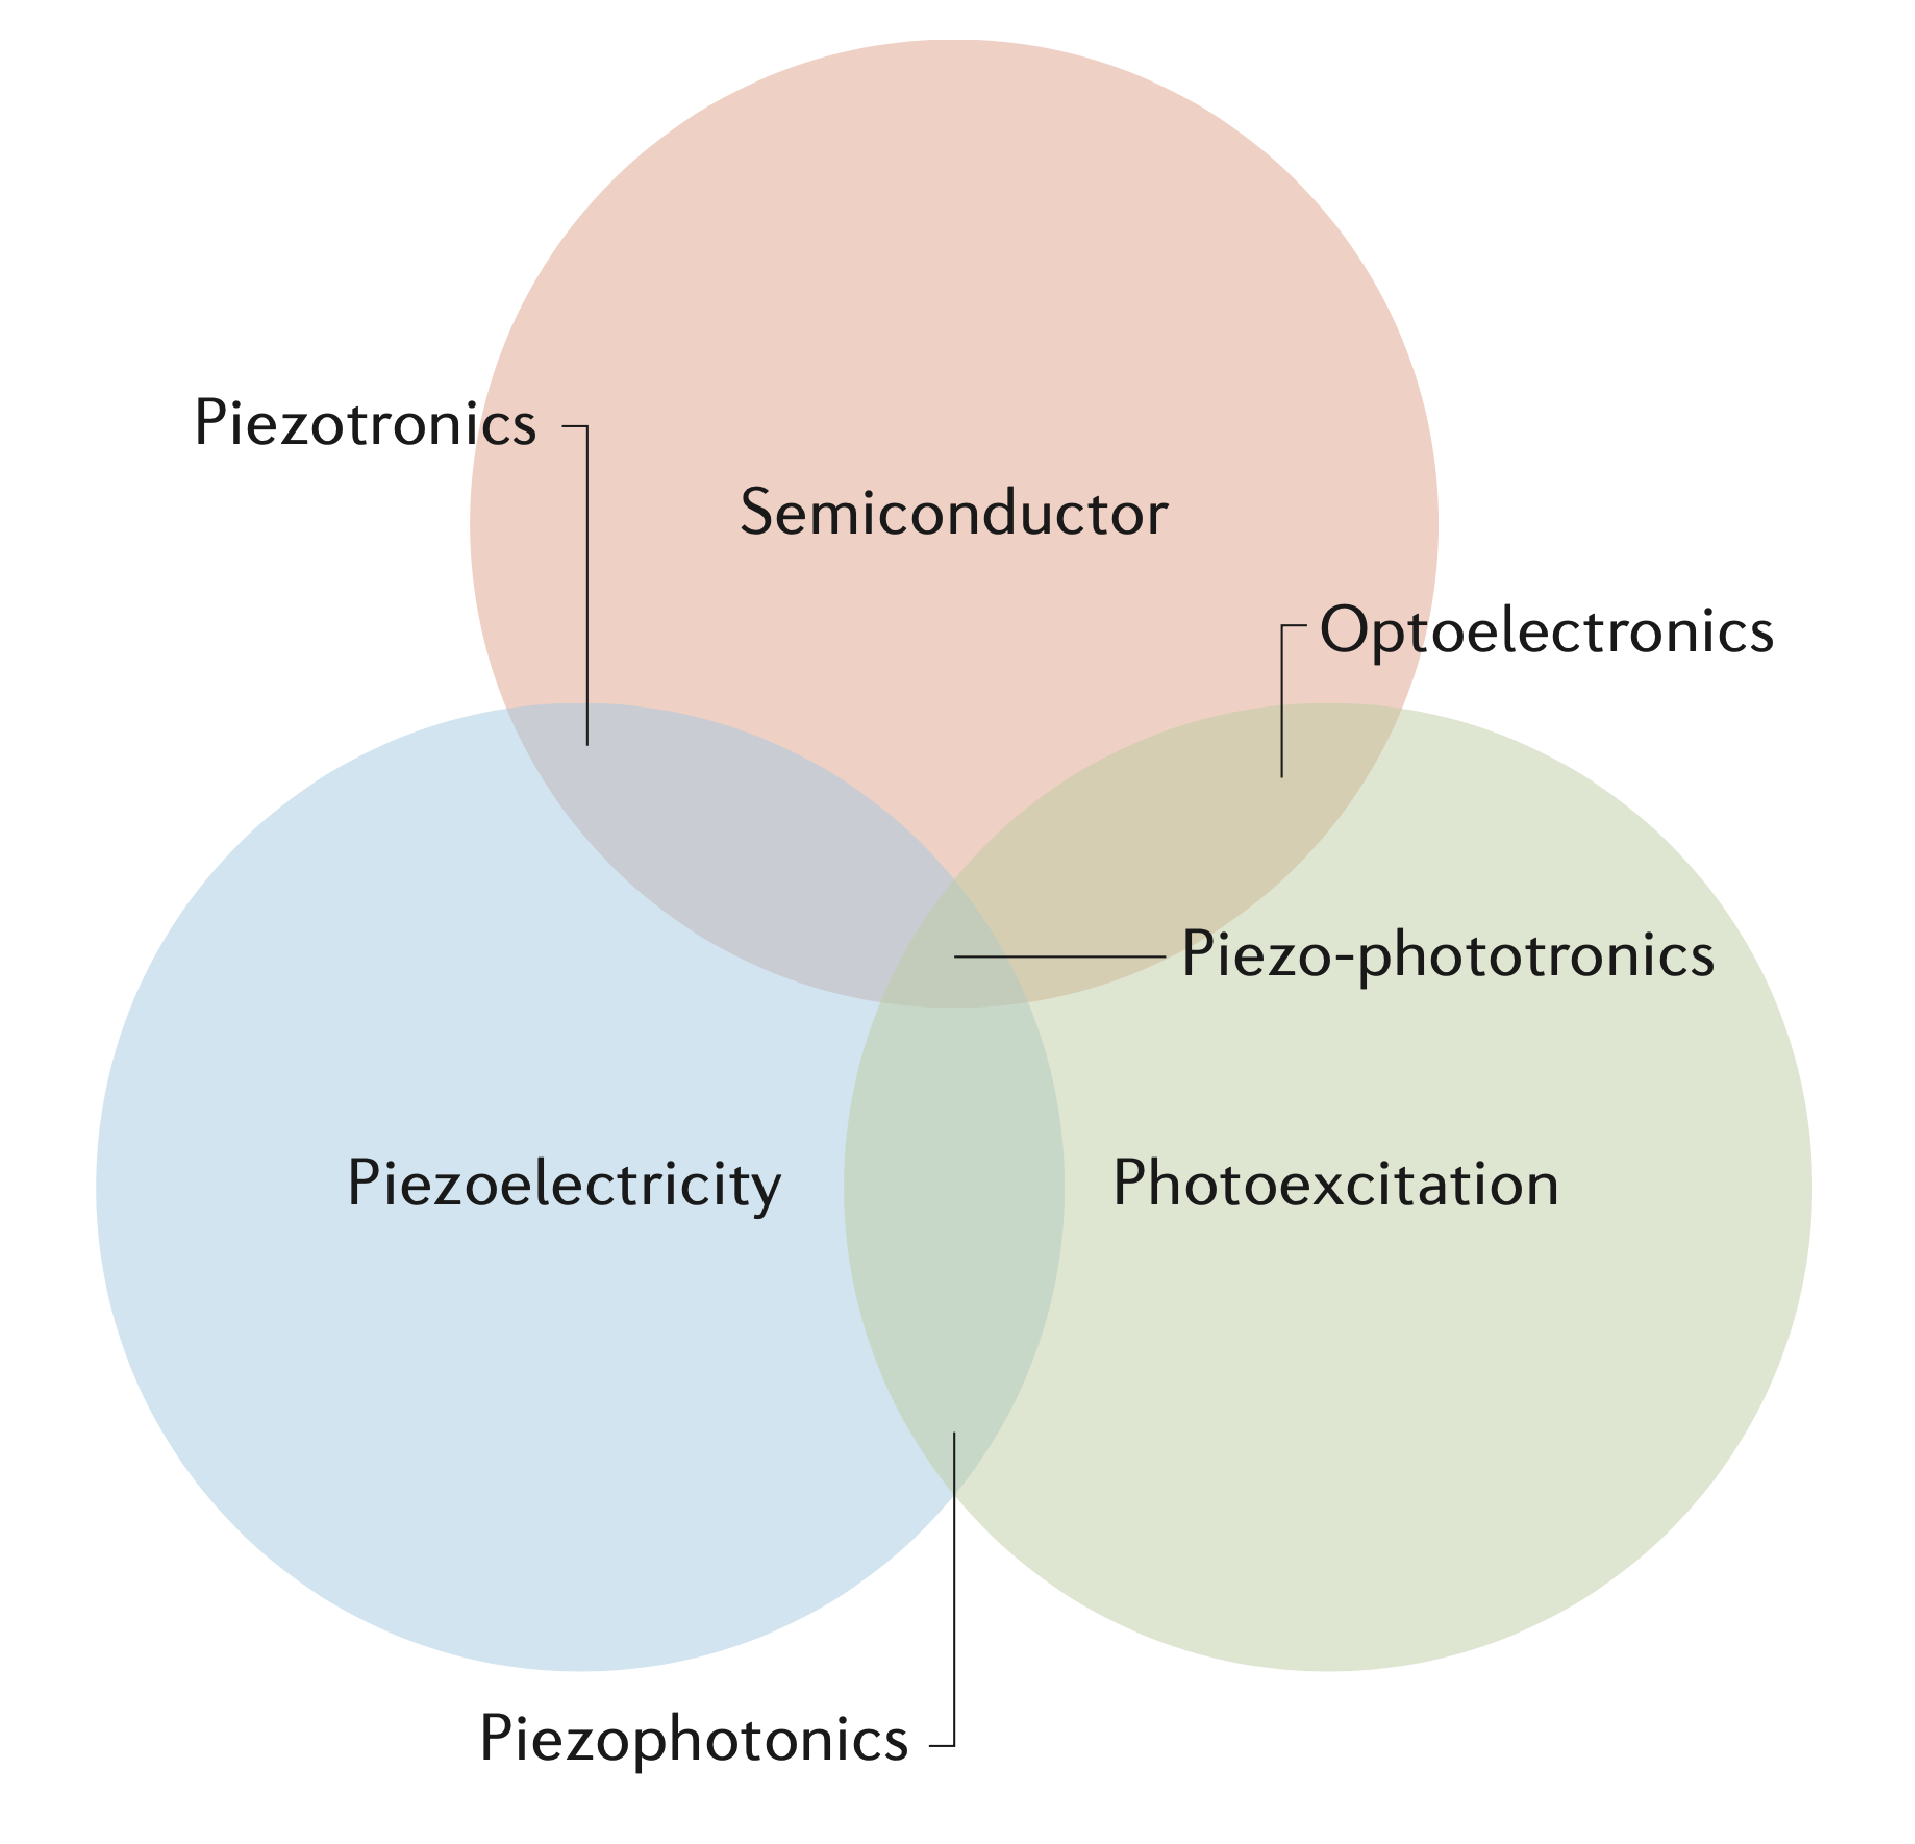
\includegraphics[width=0.7\textwidth]{ch1_1}
\caption[Coupling characteristics of piezotronics and piezo-phototronics]{Coupling characteristics of piezotronics and piezo-phototronics \protect\cite{wu2016piezotronics}}
\label{fig:1.1}
\end{figure}

The research of piezotronics \index{Piezotronics} effect mainly focus on the adjust/control the transport of carriers through piezoelectric potential \index{Piezoelectric!potential} generated by mechanical stress in semiconductor materials with piezoelectric \index{Piezoelectric!effect} properties. Therefore, according to this effect, the external stress can directly regulated the macroscopic electrical properties of piezoelectric semiconductor materials \cite{guo2017dynamic}. Among them, the Wurtzite \index{Wurtzite} crystal \index{Crystal} with hexagonal close-packed structure has good piezoelectric properties due to its non-centrosymmetric structure \cite{xin2007piezoelectricity}. Some of these materials have both piezoelectric and semiconductor properties, such as ZnO, GaN, InN and ZnS, etc., so they are widely used in piezotronics research. \autoref{fig:1.2} shows the piezoelectric potential in Wurtzite-structured ZnO nanowires. The $Zn^{2+}$ cation and $O^{2-}$ anion in ZnO are tetrahedral coordinated, and the centers of positive and negative ions overlap each other. If stress is applied at the vertices of the tetrahedron, the center of the cation and the center of the anion are displaced relative to each other and an electric dipole moment \index{Electric!dipole moment} is created (\autoref{fig:1.2}a). 

\begin{figure}[H] 
\centering    
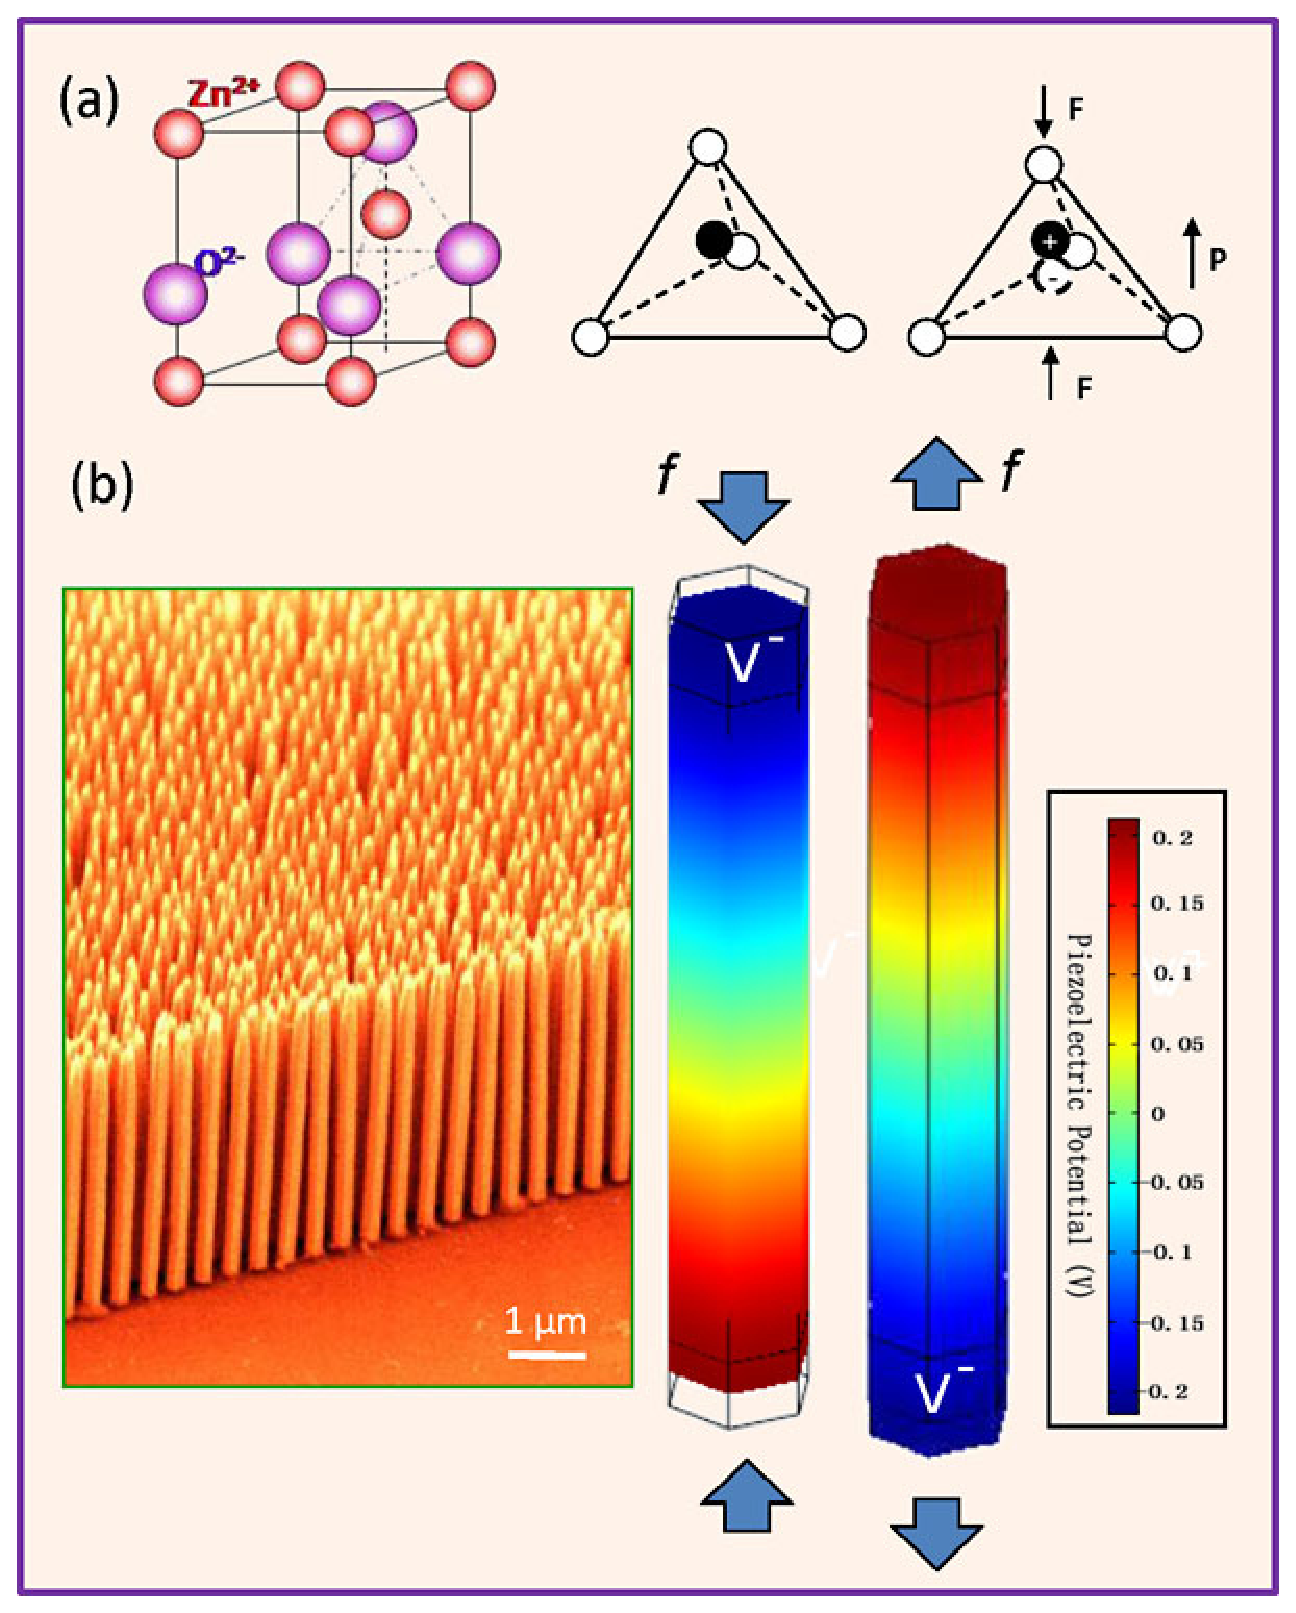
\includegraphics[width=0.7\textwidth]{ch1_2}
\caption[Piezopotential in wurtzite crystal ZnO]{Piezopotential in wurtzite crystal ZnO \protect\cite{wang2012piezotronics}}
\label{fig:1.2}
\end{figure}

The accumulation of electric dipole moments \index{Electric!dipole moment} generated by all units in the crystal \index{Crystal} leads to the generation of polarization charges \index{Polarization!charge} with the same density and opposite polarity at the interface \index{Interface} between the two ends of the crystal, resulting in a macroscopic potential along the strain \index{Strain} direction, that is, the \index{Piezoelectric!potential} piezoelectric potential (\autoref{fig:1.2}b). For a ZnO nanowire with a length of 1200 \unit{\nm} and a hexagonal length of 100 \unit{\nm}, a pulling force of 85 \unit{\nano\newton} produces a positive potential of approximately \SI{0.4}{\volt} between the two ends. When the applied force becomes compressive stress, the piezoelectric potential is reversed. The potential difference remains \SI{0.4}{\volt}, and the piezoelectric potential at both ends of the nanowire is the same in magnitude and opposite in polarity. The first systematic study of the \index{Piezoelectric!potential} piezoelectric potential in ZnO nanowires marked the beginning of the research of \index{Piezotronics} piezotronics \cite{wang2006piezoelectric}.

In piezoelectric semiconductor materials, the piezoelectric effect \index{Piezoelectric!effect} can significantly modulate the energy band \index{Energy band} structure of the material, thereby affecting the electrical properties of the material. Under the action of mechanical stress, piezoelectric polarization charges \index{Piezoelectric!polarization charge} with opposite polarities are generated at the interface \index{Interface} of the material. Piezoelectric polarization charges are distributed within a small depth from the surface \index{Surface} of the material, and they are non-mobile ionic charges located near the interface. In this case, due to the finite dielectric constant and limited doping concentration of the \index{Crystal} crystal, the free carriers can only partially shield the piezoelectric polarization \index{Piezoelectric!polarization charge} charge, but they cannot completely cancel the piezoelectric polarization charge. The piezoelectric potential \index{Piezoelectric!potential} formed by the piezoelectric polarization charges at the material interface can significantly change the contact properties of the semiconductor through the built-in \index{Electric!field} electric field, and thus the optical and electrical properties of the semiconductor contact can be directly modulated by external mechanical stress. Among them, Schottky \index{Contact!Schottky contact} contact, p-n junction, p-n heterojunction are the most common semiconductor contacts in piezoelectric semiconductor materials, so we briefly discuss the piezoelectric effects \index{Piezoelectric!effect} in these three semiconductor contacts (\autoref{fig:1.3}).

\begin{figure}[H] 
\centering    
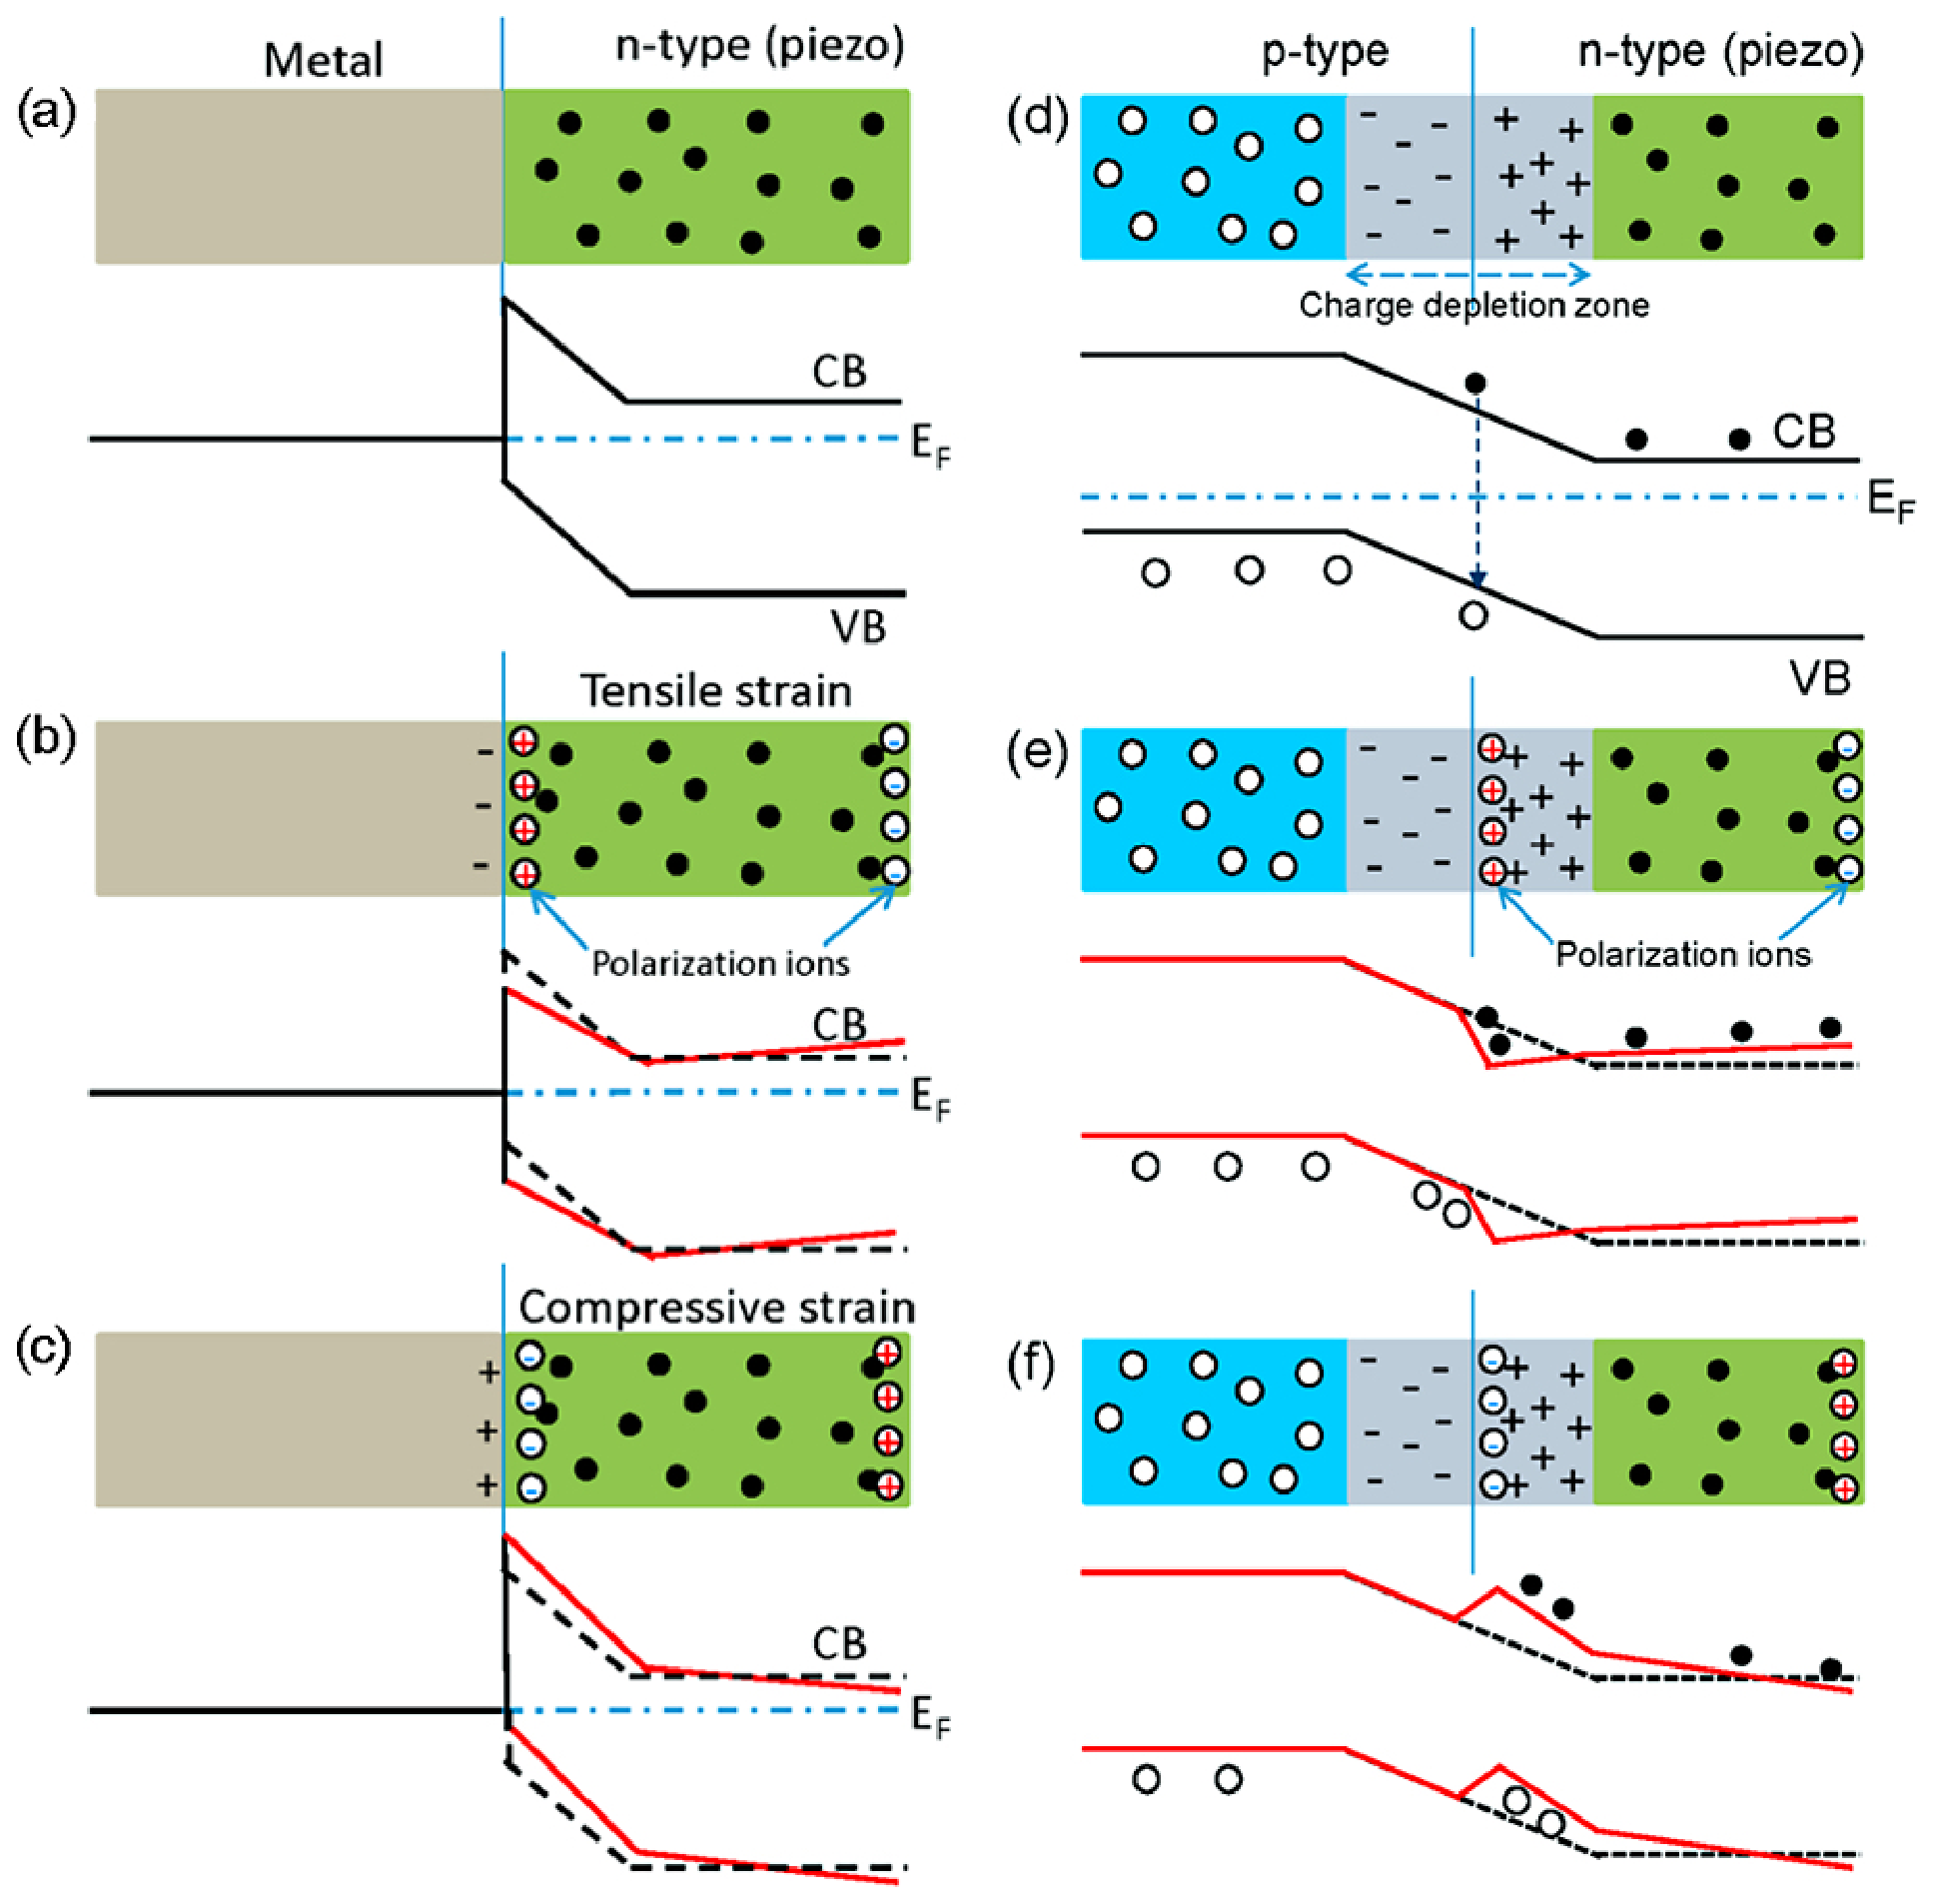
\includegraphics[width=0.9\textwidth]{ch1_3}
\caption[Energy band diagram of piezotronics effect in Schottky contact and p-n junction]{Energy band diagram of piezotronics effect in Schottky contact (a-c) and p-n junction (d-f) \protect\cite{wang2012piezotronics}}
\label{fig:1.3}
\end{figure}

In a Schottky contact \index{Contact!Schottky contact} formed by a metal material and a piezoelectric semiconductor material, strains \index{Strain} in different directions can generate piezoelectric polarization charges \index{Piezoelectric!polarization charge} with opposite polarizations at the interface \index{Interface} of the piezoelectric semiconductor material, and a negative piezoelectric polarization \index{Piezoelectric!polarization charge} charges at the metal-semiconductor material interface \index{Interface} can effectively reduce the local barrier height of Schottky \index{Contact!Schottky contact} contacts, while negative piezoelectric polarization charges \index{Piezoelectric!polarization charge} further increase the barrier height (\autoref{fig:1.3}a–c). The height of the Schottky \index{Contact!Schottky contact} barrier determines the carrier transport properties at the metal-semiconductor material interface, so we can directly modulate \index{Modulation} the electrical properties of the Schottky contact \index{Contact!Schottky contact} by external mechanical stress according to the piezotronics \index{Piezotronics} effect.

In a p-n junction composed of the same bandgap material, the interdiffusion and recombination of electrons and holes forms a depletion region in the junction region when the p-type and n-type semiconductors are in contact. The presence of such carrier-free regions can significantly enhance the piezotronics \index{Piezotronics} effect, since the piezoelectric polarization charges \index{Piezoelectric!polarization charge} here are not shielded by locally remaining free carriers. As shown in \autoref{fig:1.3}d-f, with the strain \index{Strain} applied to n-type piezoelectric semiconductor material, a net positive piezoelectric polarization charge \index{Piezoelectric!polarization charge} will be generated at the depletion region interface \index{Interface} if the doping concentration is relatively low. Piezoelectric potential \index{Piezoelectric!potential} tends to lower the local energy band \index{Energy band} slightly and introduce a slow slope into the energy band. When the applied strain \index{Strain} is in the opposite direction, the negative piezoelectric polarization charge \index{Piezoelectric!polarization charge} at the interface \index{Interface} of the depletion region raises the local energy \index{Energy band} band. The change of the energy band in the p-n junction can significantly affect the electron-hole recombination rate, which is very beneficial to improve the efficiency of LEDs. In addition, the degree of band tilt also affects the internal carrier mobility. Therefore, the piezotronics \index{Piezotronics} effect in the p-n junction can effectively tune its electrical and optical properties by external mechanical stress.

For p-n heterojunctions made of two materials with different band gaps, the piezoelectric polarization charge \index{Piezoelectric!polarization charge} also significantly affects the band distribution, as shown in \autoref{fig:1.4}. The black and red curves are used to represent the energy band \index{Energy band} diagrams of the p-n heterojunction before and after the external strain \index{Strain} in the eight cases, from which it can be seen that the transport characteristics of carriers at the interface \index{Interface} will be directly modulated \index{Modulation} by the \index{Piezoelectric!polarization charge} piezoelectric polarization charge. Take the case shown in \autoref{fig:1.4}e as an example: the height of the barrier formed at the interface \index{Interface} is reduced due to the reduction of the energy band \index{Energy band} caused by the \index{Piezoelectric!polarization charge} piezoelectric polarization charge, so that electrons can be transported across the interface \index{Interface} more efficiently. In contrast to \autoref{fig:1.4}f, the height and width of the potential barrier at the interface increase due to \index{Piezoelectric!polarization charge} piezoelectric polarization charges, hindering the transport of electrons

\begin{figure}[H] 
\centering    
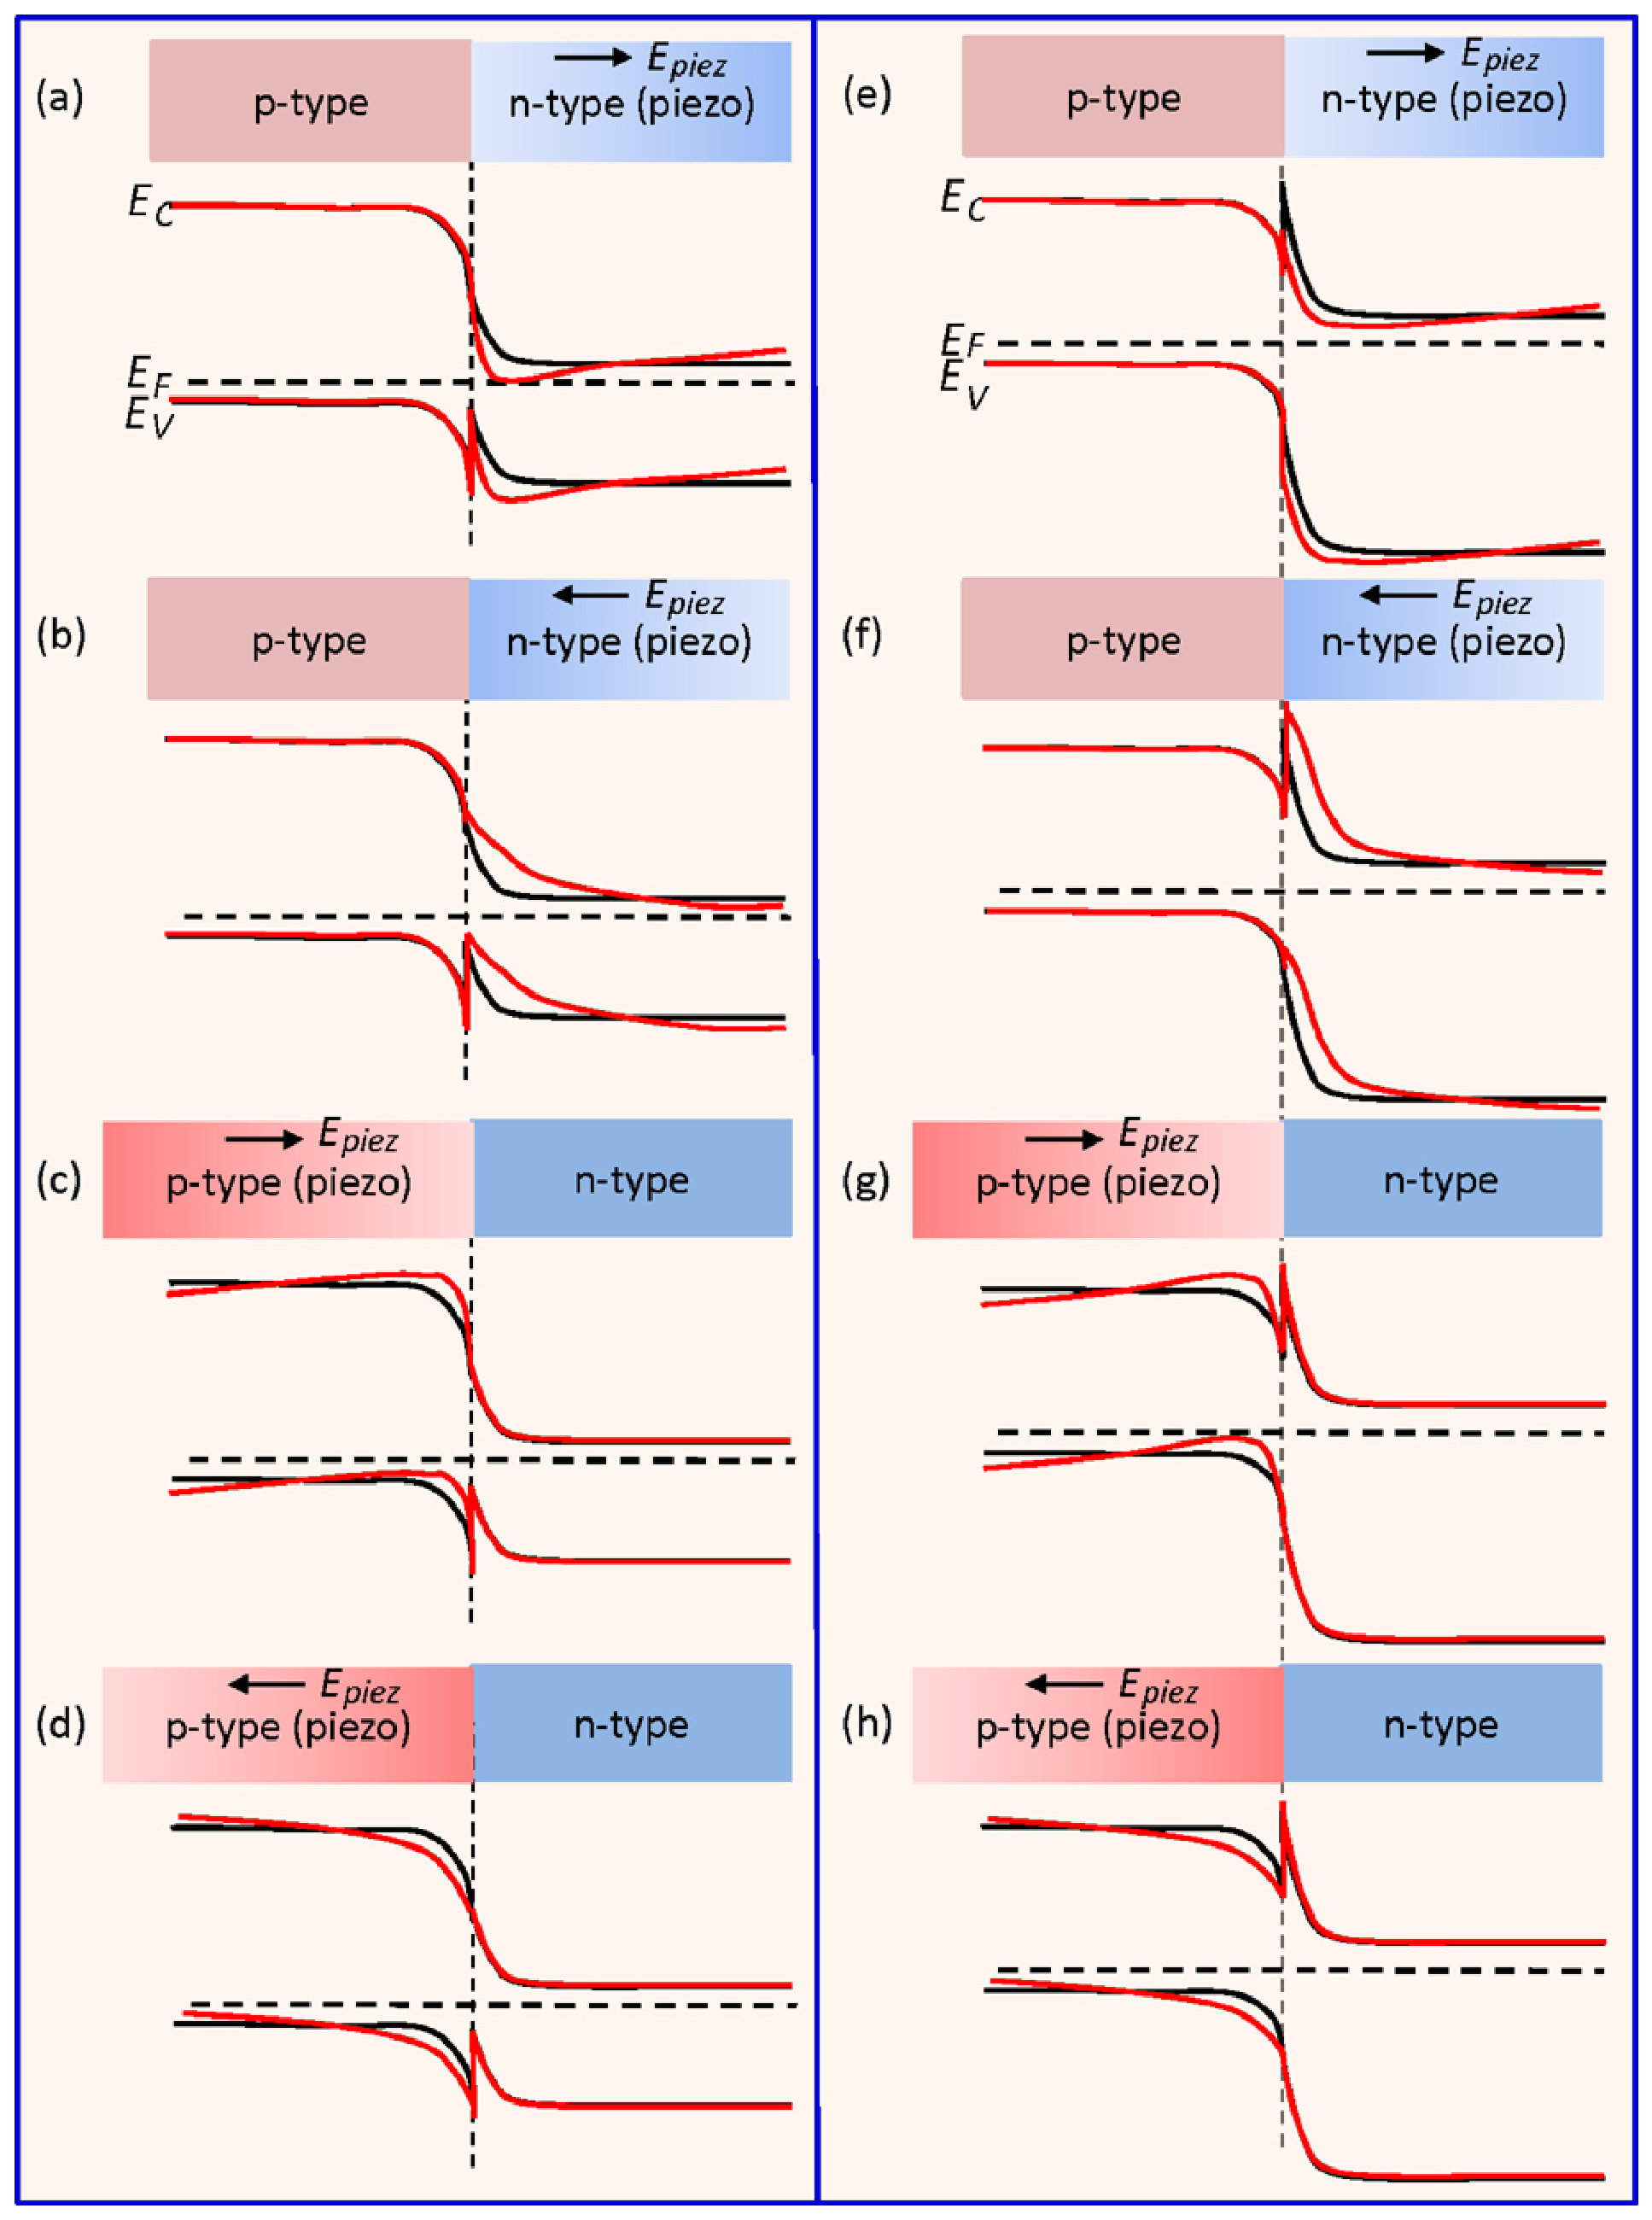
\includegraphics[width=0.9\textwidth]{ch1_4}
\caption[Energy band diagram of piezotronic effect in p-n heterojunction]{Energy band diagram of piezotronic \index{Piezotronics} effect in p-n heterojunction \protect\cite{wang2012piezotronics}}
\label{fig:1.4}
\end{figure}

\noindent across the \index{Interface} interface. For the case shown in \autoref{fig:1.4}b, the reorganization of the energy band \index{Energy band} caused by the piezoelectric polarization charge \index{Piezoelectric!polarization charge} can significantly increase the local trapping of holes and improve the luminous efficiency of the LED. But for the case of \autoref{fig:1.4}a, the reformation of the energy bands \index{Energy band} negatively affects the efficiency of the LED. Therefore, based on the piezotronics \index{Piezotronics} effect, the external strain \index{Strain} in the heterojunction can effectively tune the optoelectronic properties of the material.

Piezotronics \index{Piezotronics} transistors can be designed and fabricated based on the modulation \index{Modulation} properties of piezoelectric polarization charges \index{Piezoelectric!polarization charge} in piezoelectric semiconductor materials. For a conventional \index{Channel} n-channel metal-oxide-semiconductor field-effect transistor MOSFET (Fig. 1.5a), the drain and source are two n-type doped regions, and a thin metal insulating oxide layer is deposited on the p-type region to form the Schottky contact \index{Contact!Schottky contact} as the gate. The \index{Voltage!gate voltage} gate voltage $V_{G}$ controls the channel \index{Channel} width of the transport carriers, so the current flowing from the drain to the source under the source-drain bias voltage $V_{DS}$ is controlled by the gate voltage $V_{G}$. Similarly, for a single-channel FET (\autoref{fig:1.5}b) fabricated using semiconducting nanowire materials, the drain and source are two metal electrodes, and the current is regulated by applying a gate voltage \index{Voltage!gate voltage} on top of the nanowire. A piezotronics \index{Piezotronics} transistor is a metal-nanowire-metal structure, such as Au-ZnO-Au or Ag-ZnO-Ag, as shown in \autoref{fig:1.5}c,d. The basic principle of piezotronics \index{Piezotronics} transistor is to generate a piezoelectric potential \index{Piezoelectric!potential} at the interface \index{Interface} of the semiconductor by applying external \index{Strain} strain, thereby regulating the local energy band \index{Energy band} at the contact, and finally realizing the control of the carrier transport characteristics at the metal-semiconductor interface. Therefore, unlike conventional MOSFETs, in piezotronics \index{Piezotronics} transistor based on the piezoelectric \index{Piezoelectric!effect} effect, the externally applied gate voltage \index{Voltage!gate voltage} that controls the channel \index{Channel} width is replaced by a \index{Strain} strain-generated piezoelectric \index{Piezoelectric!potential} potential, thus eliminating the "gate". Piezotronics \index{Piezotronics} transistor are a new type of transistors that replace voltage control with external \index{Strain} strain/stress control, and have broad application prospects.

\begin{figure}[H] 
\centering    
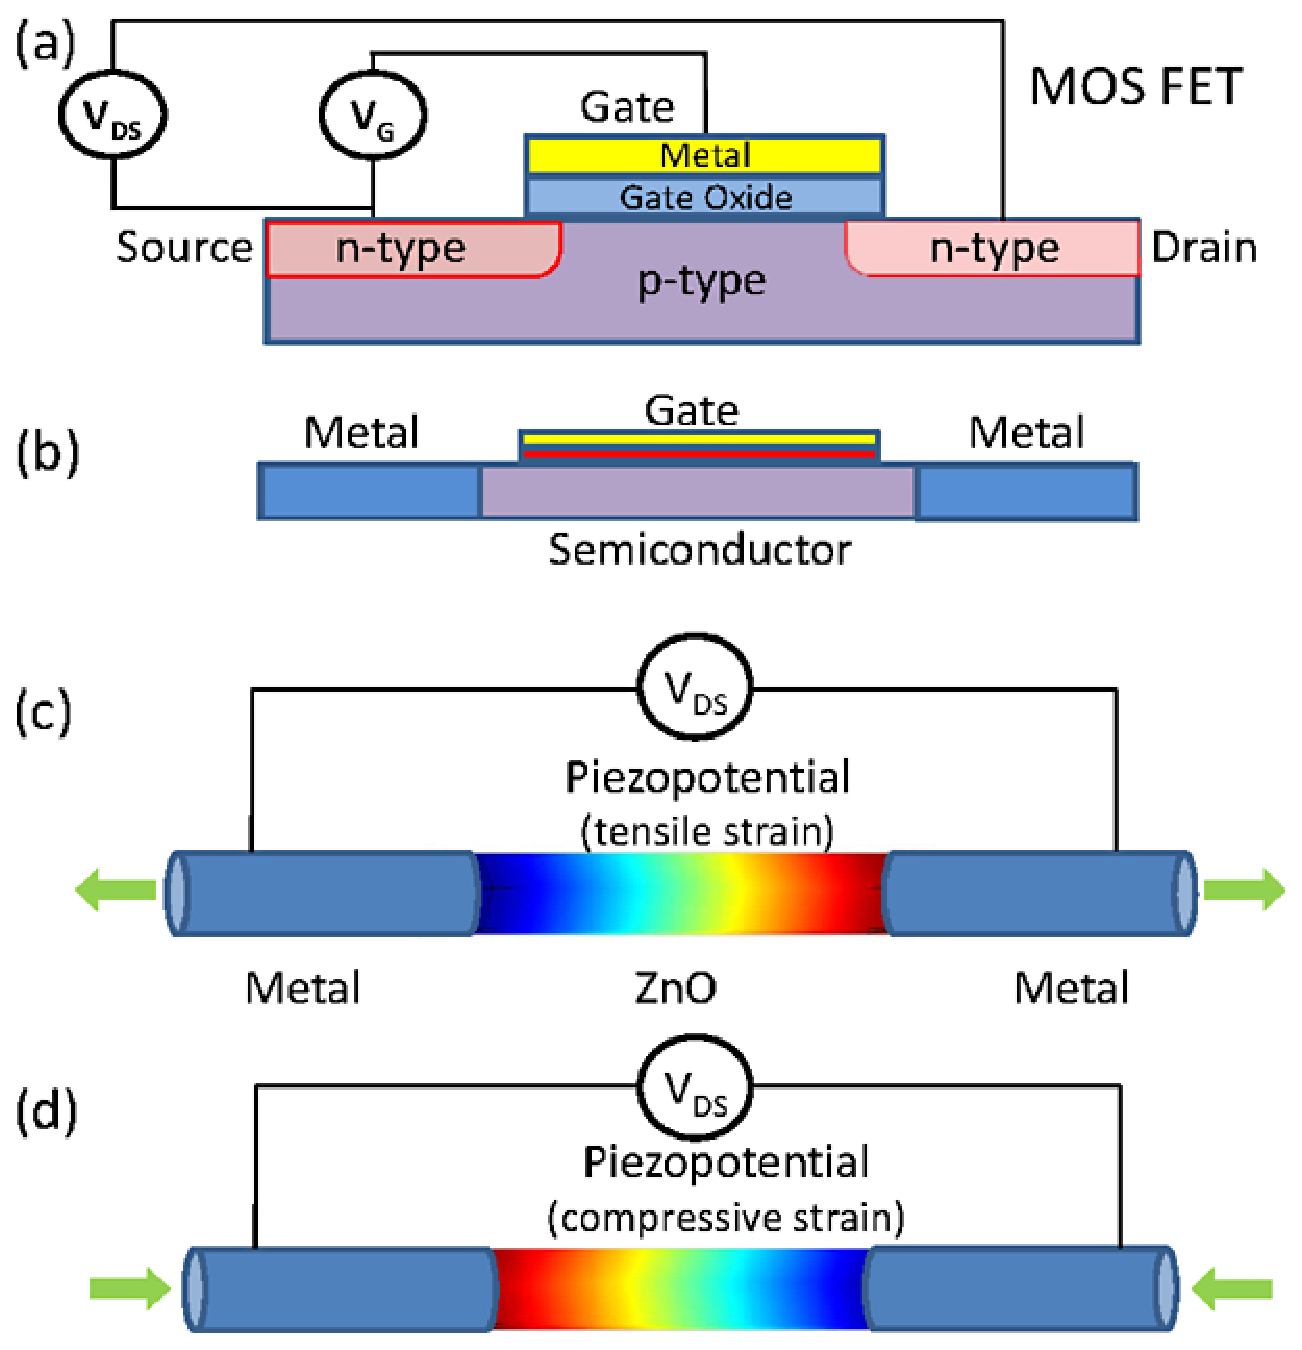
\includegraphics[width=0.7\textwidth]{ch1_5}
\caption[Working principle of piezotronics transistor]{Working principle of piezotronics transistor. (a) The n-channel MOSFET; (b) The semiconductor nanowire FET; The piezotronics transistor with tensile strain (c) and compressive strain (d) \protect\cite{wang2012piezotronics}}
\label{fig:1.5}
\end{figure}

\subsection{Application prospect of piezotronics effect}

The study of piezotronics \index{Piezotronics} effects, ie the study of the coupling properties of piezoelectric and semiconductor properties in piezoelectric semiconductor materials, has given rise to a whole new range of applications. By using piezoelectric potential \index{Piezoelectric!potential} as the gate voltage \index{Voltage!gate voltage} to modulate \index{Modulation} the transport properties of electrons, researchers have fabricated transistors, sensors and smart devices driven and controlled by external stress, including piezoelectric potential \index{Piezoelectric!potential} gate field effect transistors \cite{wang2006piezoelectric-nl}, piezoelectric potential \index{Piezoelectric!potential} gated diodes \cite{he2007piezoelectric}, strain sensor \cite{zhou2008flexible}, force/flow sensor \cite{fei2009piezoelectric}, hybrid field effect transistor \cite{liu2010piezopotential}, piezoelectric logic gate \cite{wu2010strain}, electromechanical memory \cite{wu2011piezotronic}, etc. Piezotronics \index{Piezotronics} devices have been regarded as a new class of semiconductor devices with important applications in sensors, human-machine interfaces, MEMS, nanorobots, and flexible electronics (\autoref{fig:1.6}).

\begin{figure}[H] 
\centering    
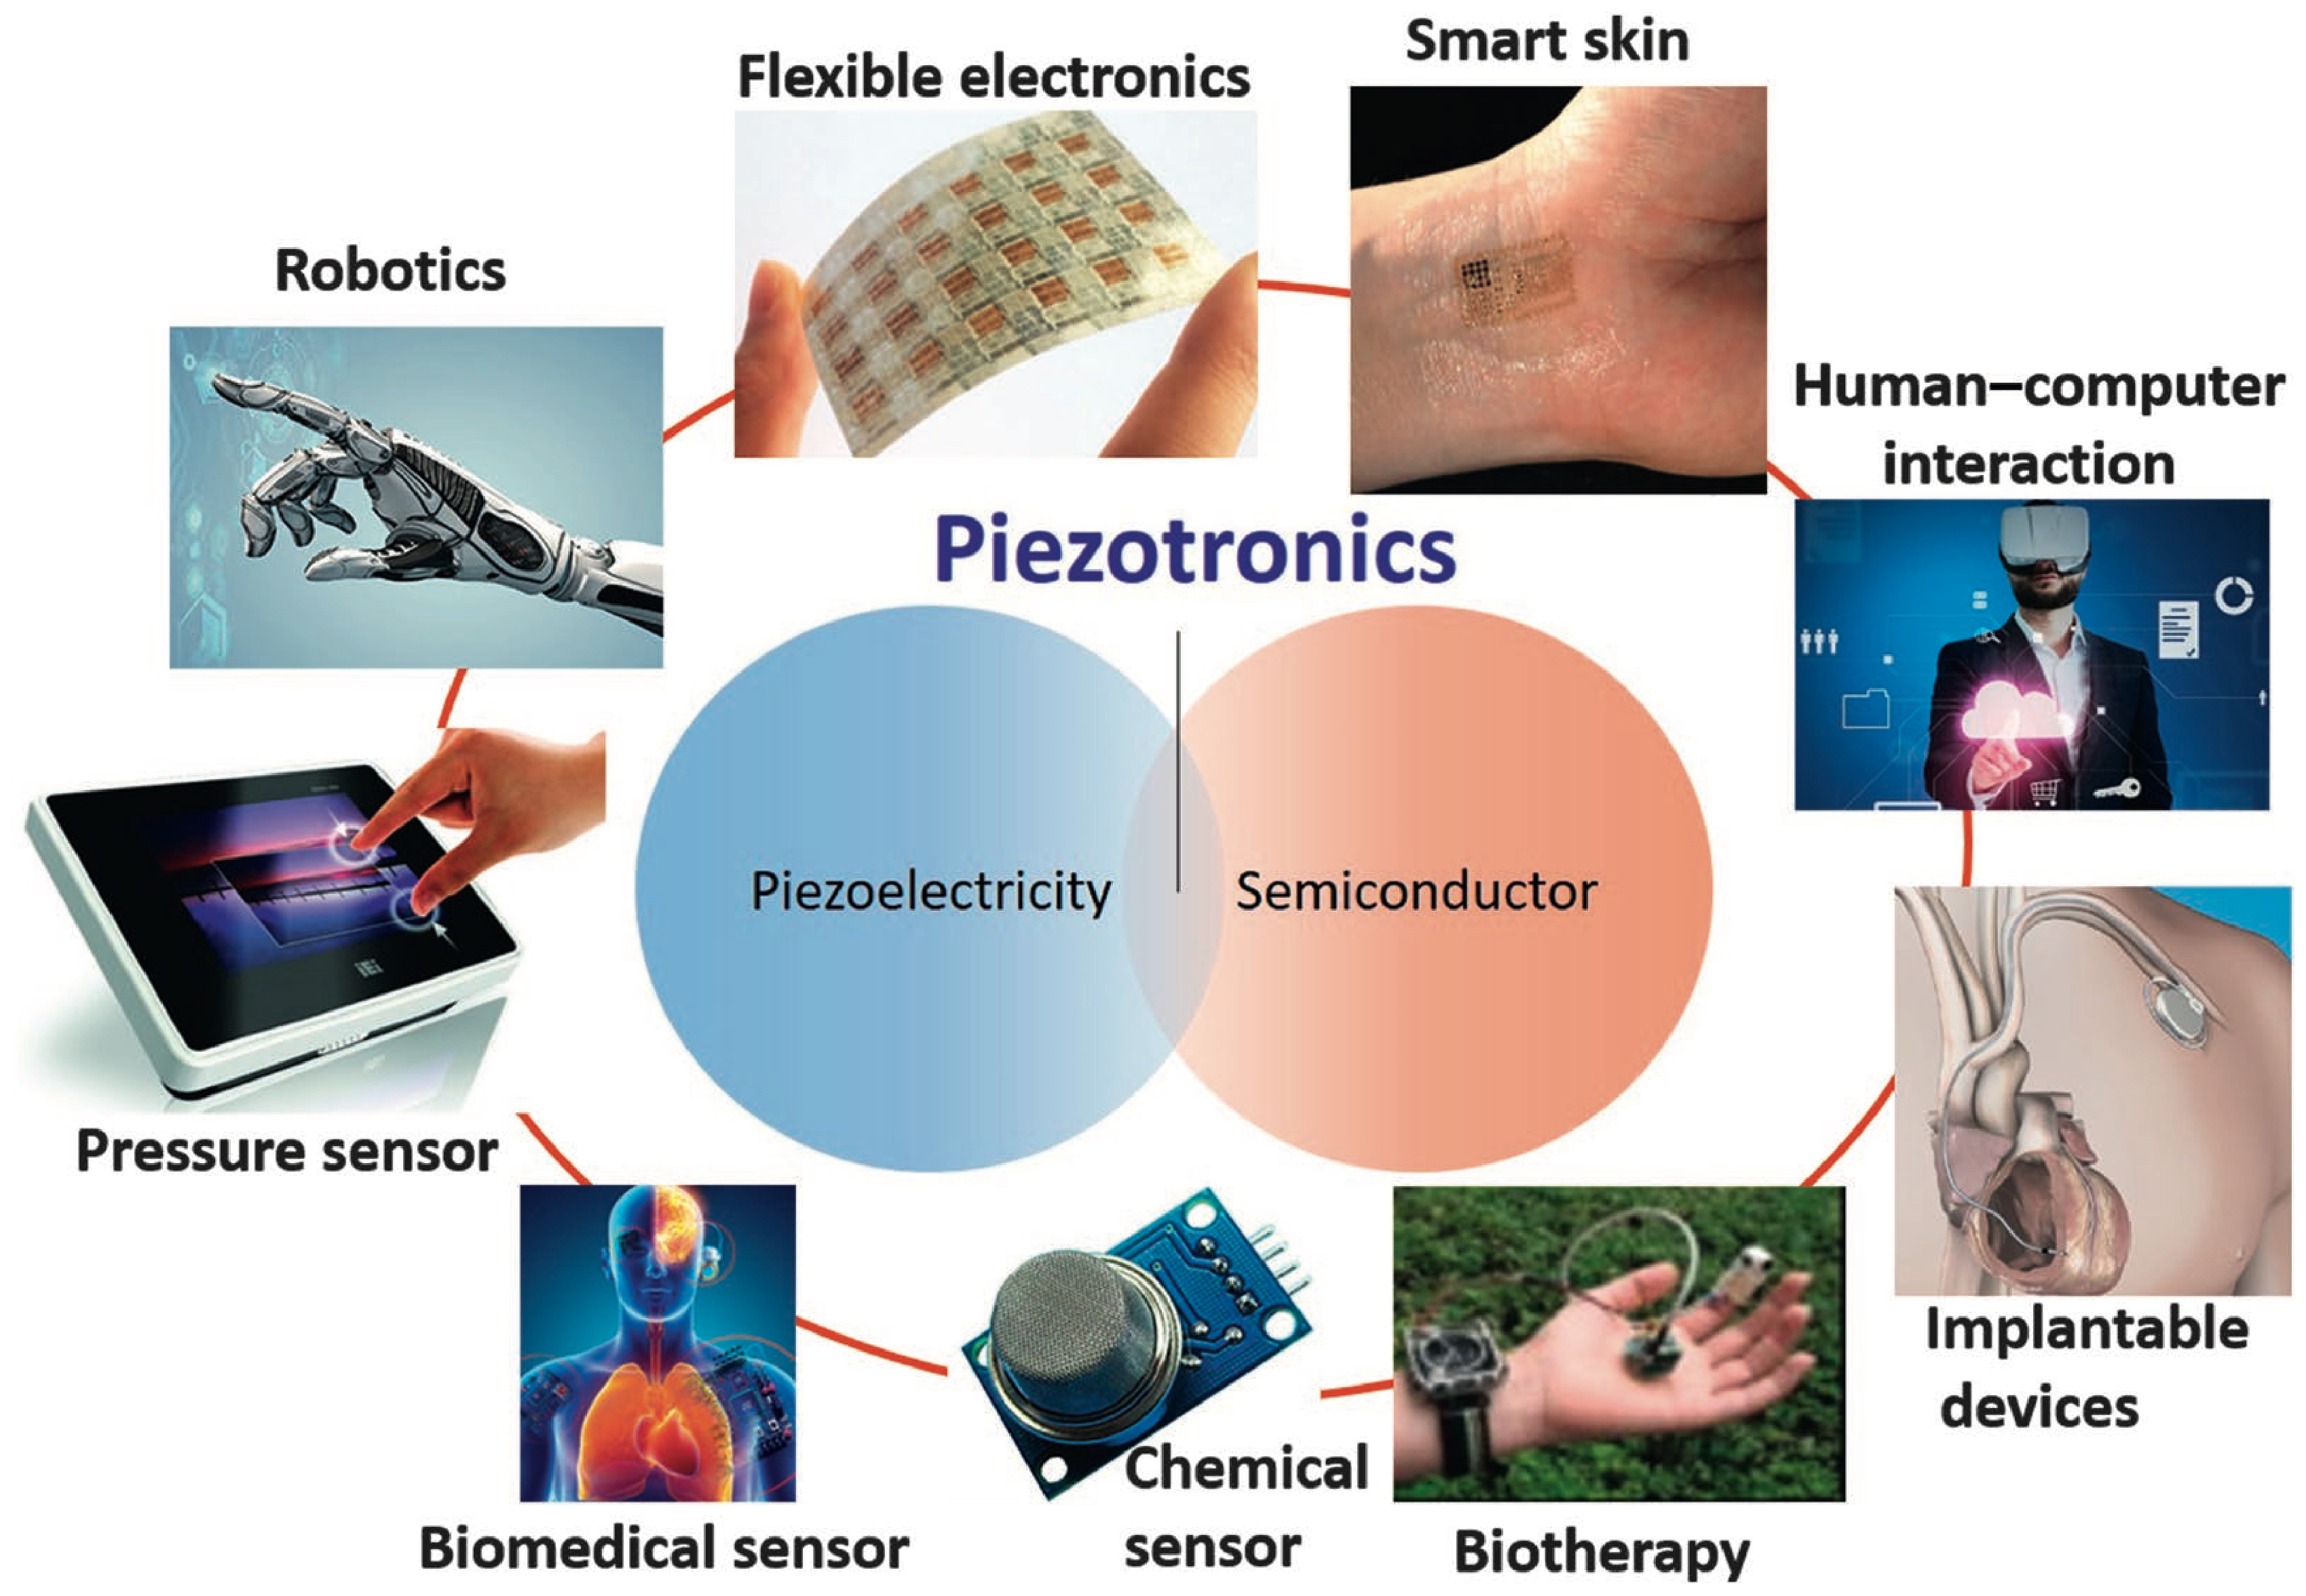
\includegraphics[width=0.9\textwidth]{ch1_6}
\caption[The application prospects and future prospects of piezotronics]{The application prospects and future prospects of piezotronics \protect\cite{hu2018piezotronic}}
\label{fig:1.6}
\end{figure}

%********************************** %Second Section  *************************************
\section{Piezotronics effects in III-V nitrides} 
\subsection{Crystal structure and polarization properties of III-V nitrides}

Group III-V nitride \index{Nitride} materials are compound semiconductor materials formed by group III elements Al, Ga, In and group V elements N, such as GaN, InN, AlN and multi-element alloy materials ($In_{x}Ga_{1-x}N$, $Al_{x}Ga_{1-x}N$, etc.). There are usually two different lattice structures of hexagonal \index{Wurtzite} wurtzite (Wurtzite) and cubic sphalerite (Zinc-blende). Among them, the nitride crystal \index{Crystal} of wurtzite structure is more stable and is widely used in semiconductor materials. This research focuses on GaN, AlN and $Al_{x}Ga_{1-x}N$  semiconductor materials. 

\begin{figure}[H] 
\centering    
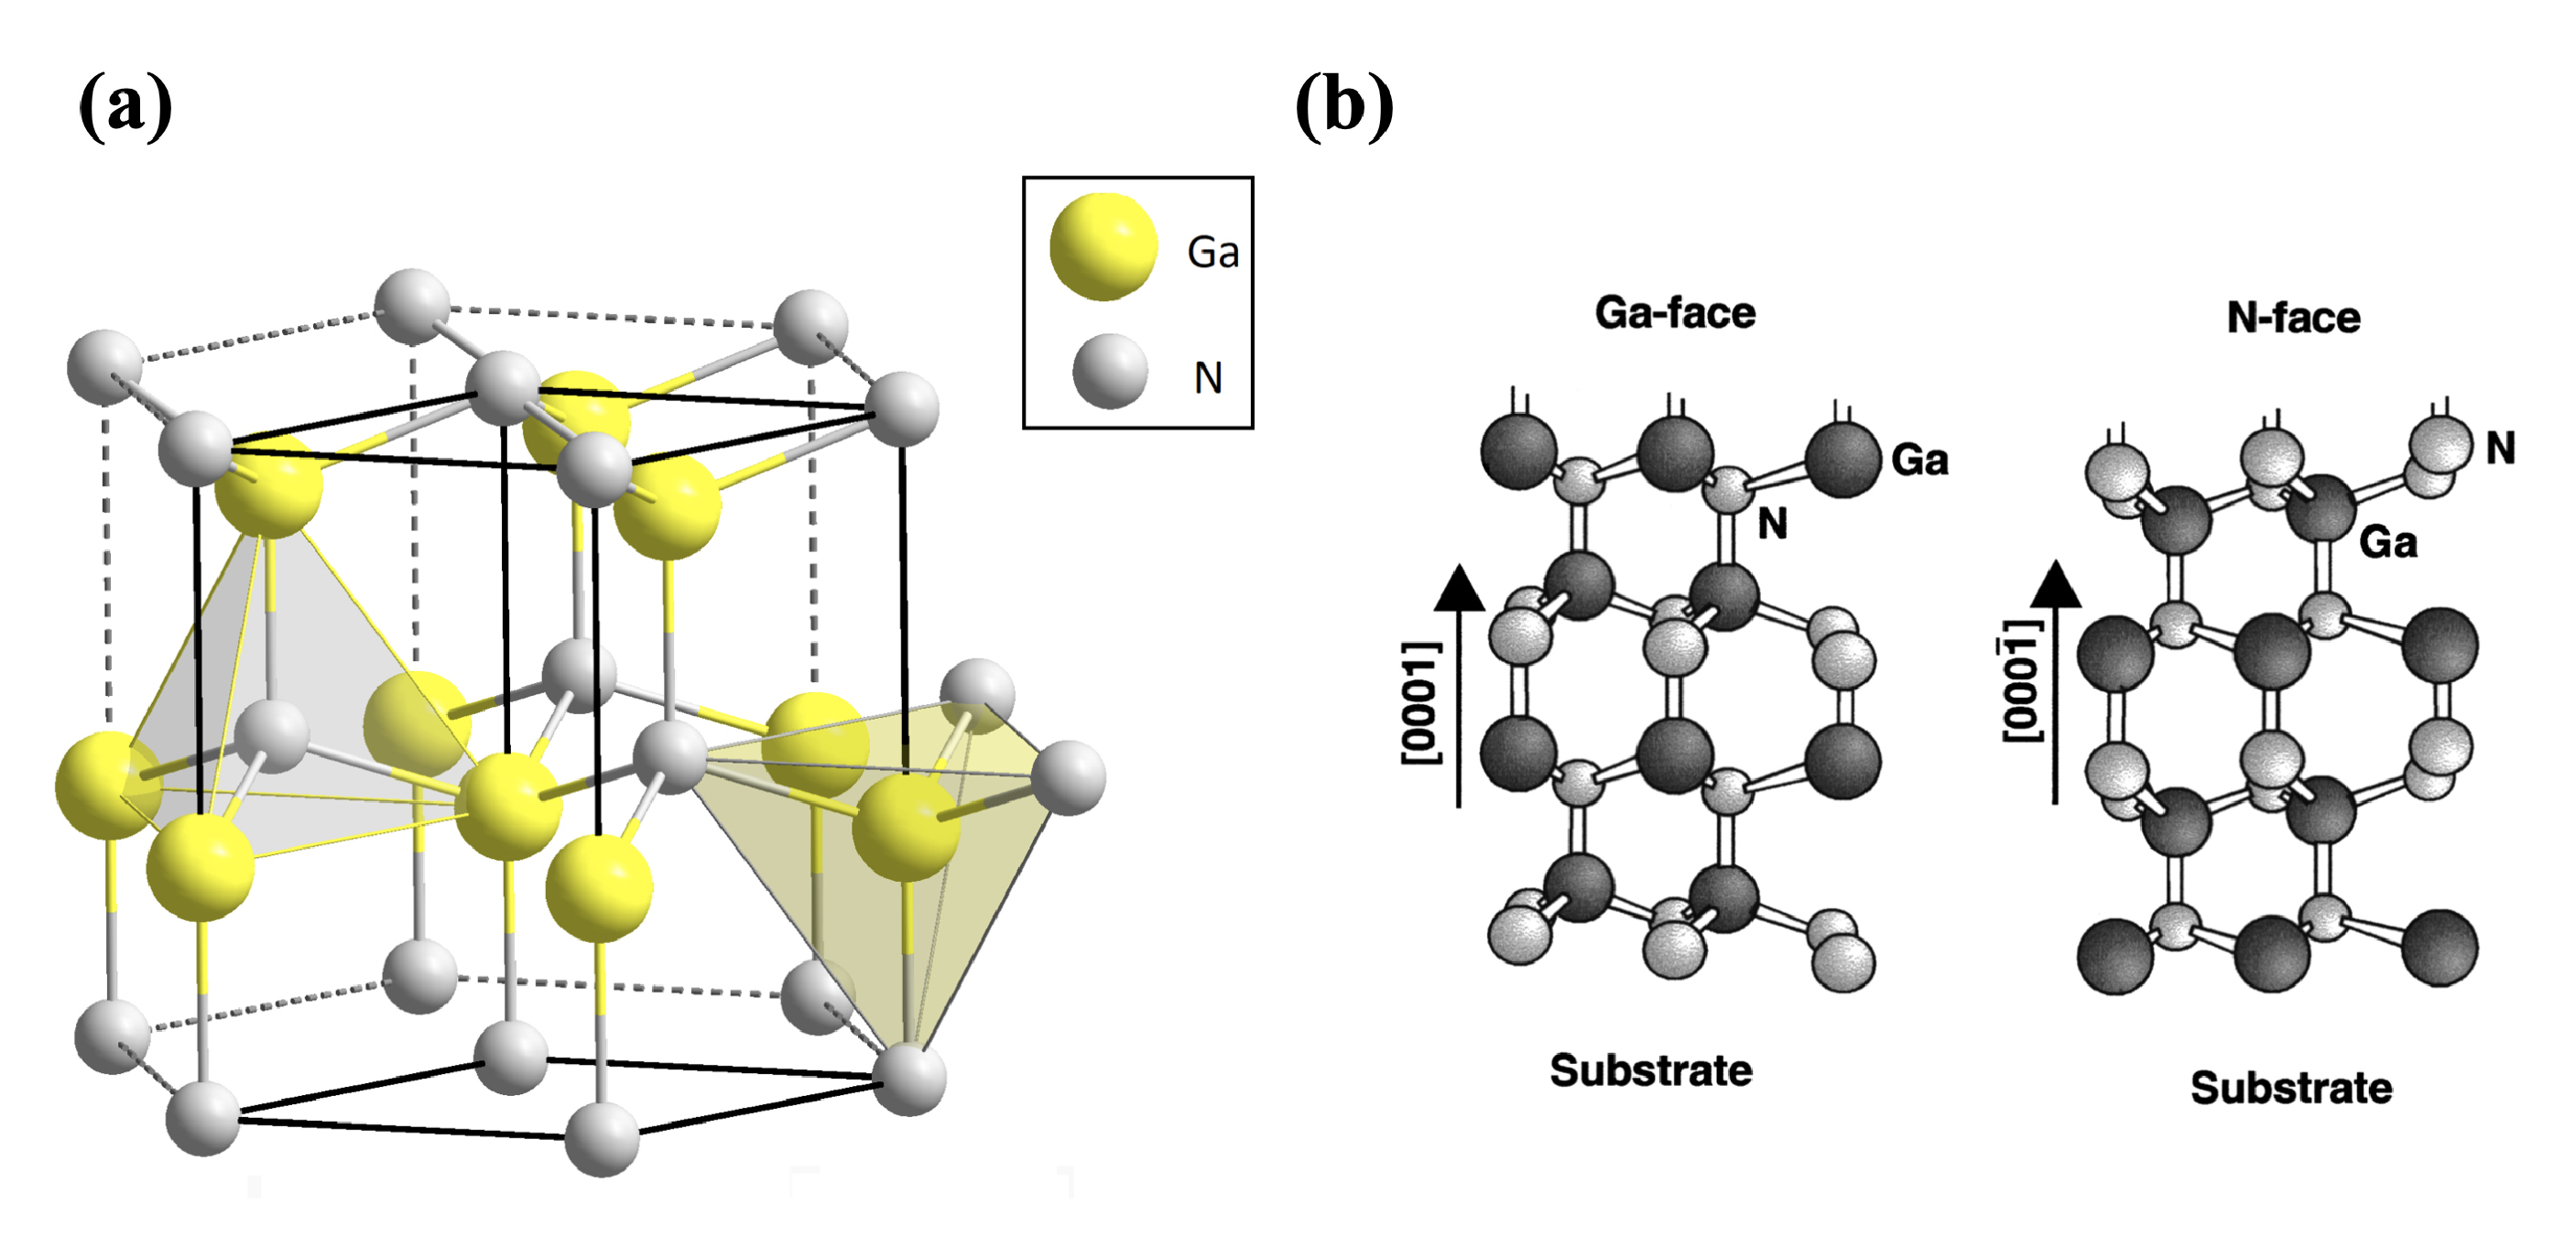
\includegraphics[width=0.9\textwidth]{ch1_7}
\caption[The wurtzite crystal structure of GaN material and the polarization characteristics of the Ga and N plane]{The wurtzite crystal structure of GaN material and the polarization characteristics of the Ga and N plane}
\label{fig:1.7}
\end{figure}

\autoref{fig:1.7}a shows the wurtzite \index{Wurtzite} structure of GaN \index{Crystal} crystal. Since the wurtzite structure of GaN crystal \index{Crystal} belongs to the non-centrosymmetric crystal, the crystal pole axis is the c-axis, and the atomic layers are are aligned along the c-axis from two different directions $[0001]$ and $[000\overline{1}]$, thus forming two distinct polar faces. It can be seen from \autoref{fig:1.7}b that when accumulating from the bottom to the top along the $[0001]$ direction, the top is the Ga atomic plane, which causes the Ga surface \index{Surface} polarity to be generated on the surface of the material; when accumulating from the bottom to the top along the $[000\overline{1}]$ direction, the top is the N atomic plane so that the N-plane polarity is generated on the surface of the material \cite{hellman1998polarity}. Since the electronegativity \index{Electronegativity} of negative ions formed by N atoms is stronger than that of positive ions formed by Ga atoms, a built-in electric field \index{Electric!field} will be generated. The direction of the electric field is from Ga atoms to N atoms along the c-axis. This phenomenon is called Spontaneous \index{Spontaneous polarization} Polarization \index{Polarization!effect} effect of GaN crystal \cite{sacconi2001spontaneous,yu1999spontaneous}. Generally, the spontaneous polarization direction of Ga-plane polarity GaN crystals is that the surface points to the inside, and the upper surface of the material gathers negative polarized charges and is negatively charged. The spontaneous polarization \index{Spontaneous polarization} direction of N-plane polarity GaN crystals \index{Crystal} is that the interior points to the surface. The upper surface \index{Surface} is positively charged by accumulating positive polarized charges. This phenomenon is more obvious in the Al-N atomic pair, so the same spontaneous polarization effect also exists in the AlGaN compound semiconductor material. In addition, if the GaN lattice is subjected to compressive or tensile deformation \index{Deformation} due to mechanical stress, it will cause lattice strain \index{Lattice!strain} within a certain range. At this time, the centers of $Ga^{+}$ ions and $N^{-}$ ions will be separated to form an \index{Electric!dipole moment} electric dipole moment, and the surface \index{Surface} of the material will also appear polarization \index{Polarization!charge} charge. This effect is called Piezoelectric Polarization \index{Piezoelectric!polarization} effect of GaN crystal \cite{sacconi2001spontaneous,yu1999spontaneous}. Therefore, the \index{Crystal} GaN crystal is also known as piezoelectric semiconductor material.

GaN and its corresponding Al and In composition compound semiconductor materials have unique material and electrical properties due to \index{Piezoelectric!effect} piezoelectric effect, such as changing Al composition in AlGaN/GaN heterojunction to adjust the degree of lattice mismatch \index{Lattice!mismatch} between AlGaN and GaN so as to generate corresponding \index{Piezoelectric!polarization charge} piezoelectric polarization charges, thereby modulating \index{Modulation} the energy band \index{Energy band} at the heterojunction and forming a two-dimensional electron gas (2DEG) \index{Two-dimensional electron gas (2DEG)} with high density and high \index{Electron mobility} electron mobility. The method of modulating the energy band \index{Energy band} and electrical properties by the polarization effect \index{Polarization!effect} is called Polarization Engineering \index{Polarization!engineering} \cite{hao2016nitride,jena2010polarization}. \autoref{fig:1.8} shows the strain-induced \index{Strain} piezoelectric polarization charge \index{Piezoelectric!polarization charge} density and the direction of spontaneous \index{Spontaneous polarization} and piezoelectric polarization \index{Piezoelectric!polarization} in an AlGaN/GaN heterojunction with Ga- and N-plane polarities. Therefore, III-V nitride \index{Nitride} compound semiconductor materials couple piezoelectric properties and semiconductor properties, and exhibits significant piezotronics \index{Piezotronics} effects \cite{pan2019piezotronics,sha2019iii,wang2018piezotronics}. Piezoelectric polarization charges generated at the interface by external strain can modulate the energy band of the heterojunction and the two-dimensional electron gas (2DEG) concentration \index{Two-dimensional electron gas (2DEG)} in the potential \index{Potential!well} well \cite{lev2018k}. In recent years, several studies have shown that the \index{Strain} strain-induced piezoelectric polarization charge at the AlGaN/GaN heterojunction interface \index{Interface} has been used to tune the piezoelectric nanowires \cite{wang2016piezotronic}, LEDs \cite{huang2016piezo,liu2020piezo,guo2021enhanced} and HEMTs \cite{liu2017electrical,jiang2017piezotronic,zhu2019piezotronic} based on the piezotronics effect.

\begin{figure}[H] 
\centering    
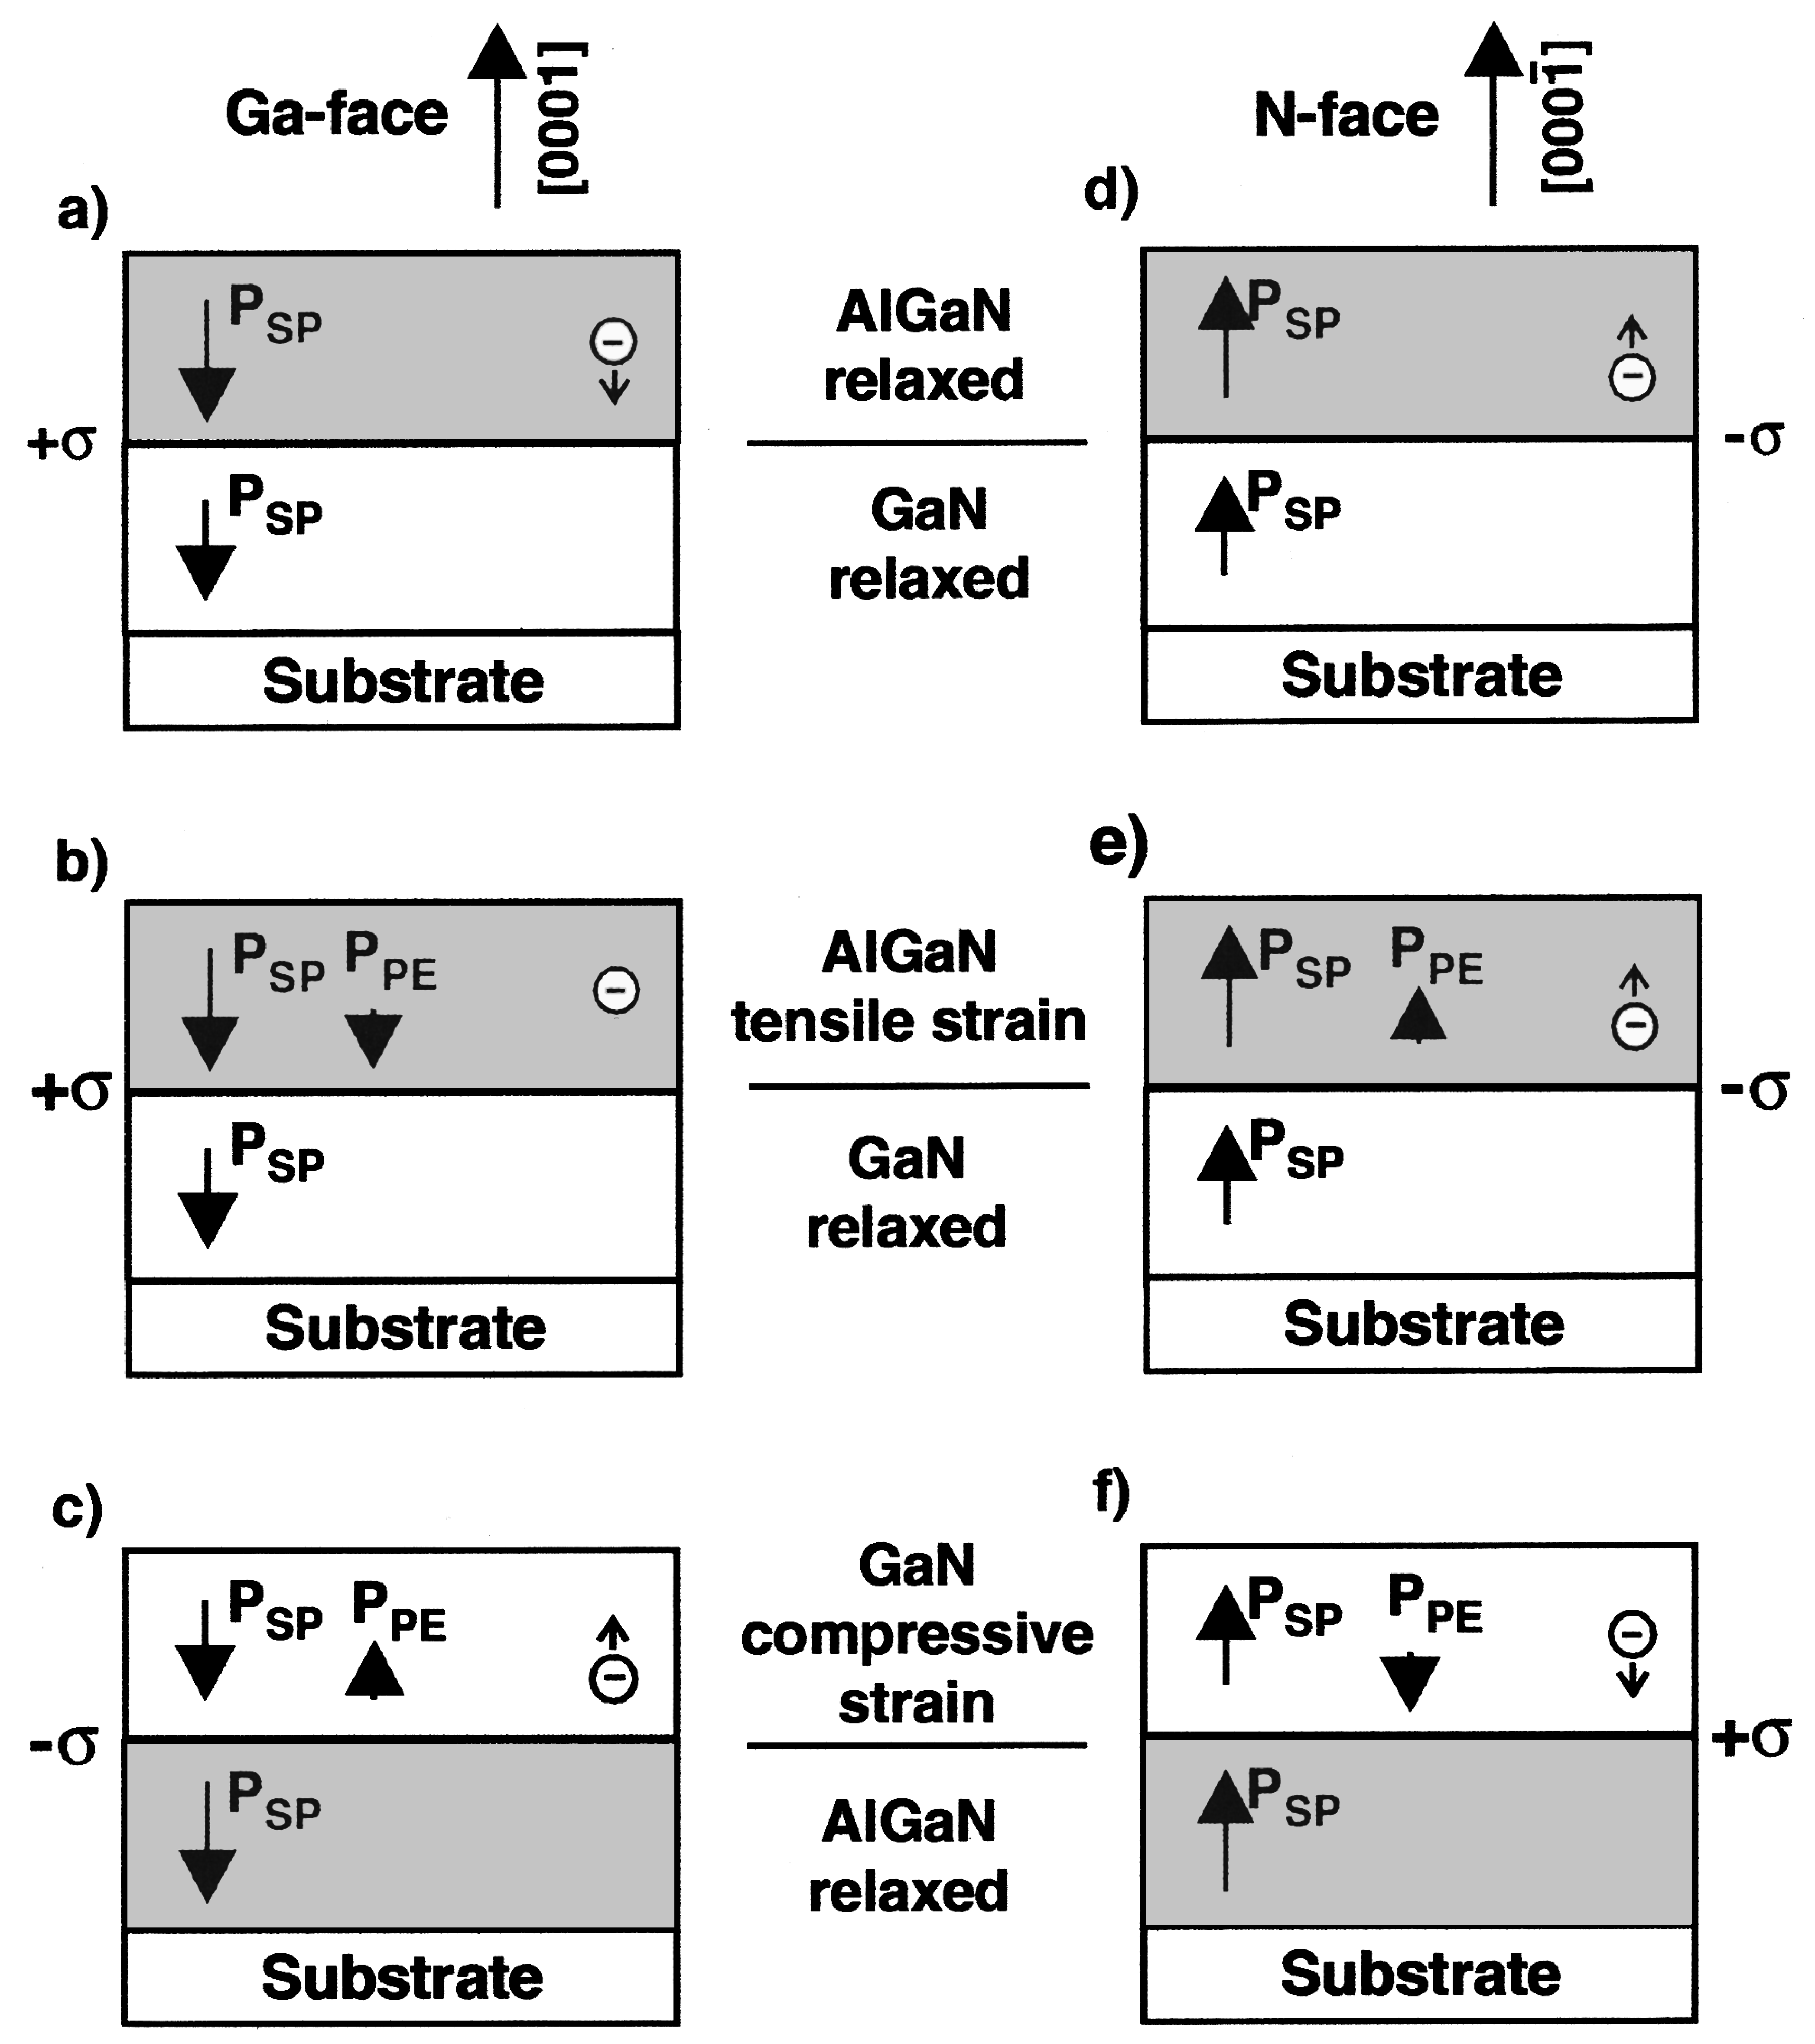
\includegraphics[width=0.9\textwidth]{ch1_8}
\caption[Polarization charge in AlGaN/GaN heterojunction with Ga-plane and N-plane polarity]{Polarization charge in AlGaN/GaN heterojunction with Ga-plane and N-plane polarity \protect\cite{ambacher1999two}}
\label{fig:1.8}
\end{figure}

\subsection{Application of piezotronics effect in III-V nitride}

Piezotronics \index{Piezotronics} effects have been widely used in the study of III-V \index{Nitride} nitrides. Wang et al. were the first to study the piezotronics effect in AlGaN/AlN/GaN heterostructured \index{AlGaN/AlN/GaN heterojunction} microwires and applied it as a novel approach to tune the physical properties of \index{Heterojunction electron gas (HEG)} heterojunction electron gas (HEG) \cite{wang2016piezotronic}. Unlike conventional approaches to tune HEG properties by changing the alloy composition or controlling the thickness of the heterojunction film, this work exploits \index{Strain} strain-induced piezoelectric polarization charges \index{Piezoelectric!polarization charge} to modify the local energy band \index{Energy band} distribution at the heterojunction, as shown in \autoref{fig:1.9}. By introducing piezotronics \index{Piezotronics} effects into AlGaN/AlN/GaN heterostructure microwires, the electrical conductivity \index{Electrical!conductivity} of \index{Heterojunction electron gas (HEG)} HEG increases by 165$\%$ at -1.78$\%$ compressive strain and decreases by 48$\%$ at 1.78$\%$ tensile strain at room temperature. This modulation \index{Modulation} is further enhanced by 890$\%$ and 940$\%$ under compressive and tensile strains, respectively, due to the enhanced piezoelectric effect \index{Piezoelectric!effect} at lower ambient temperature of 77 \unit{\kelvin}. This study provides insight into the piezotronics \index{Piezotronics} effects of low-dimensional electron gas in heterostructured nanomaterials with potential applications in HEMT \index{HEMT} and \index{MEMS} MEMS/NEMS.

\begin{figure}[H] 
\centering    
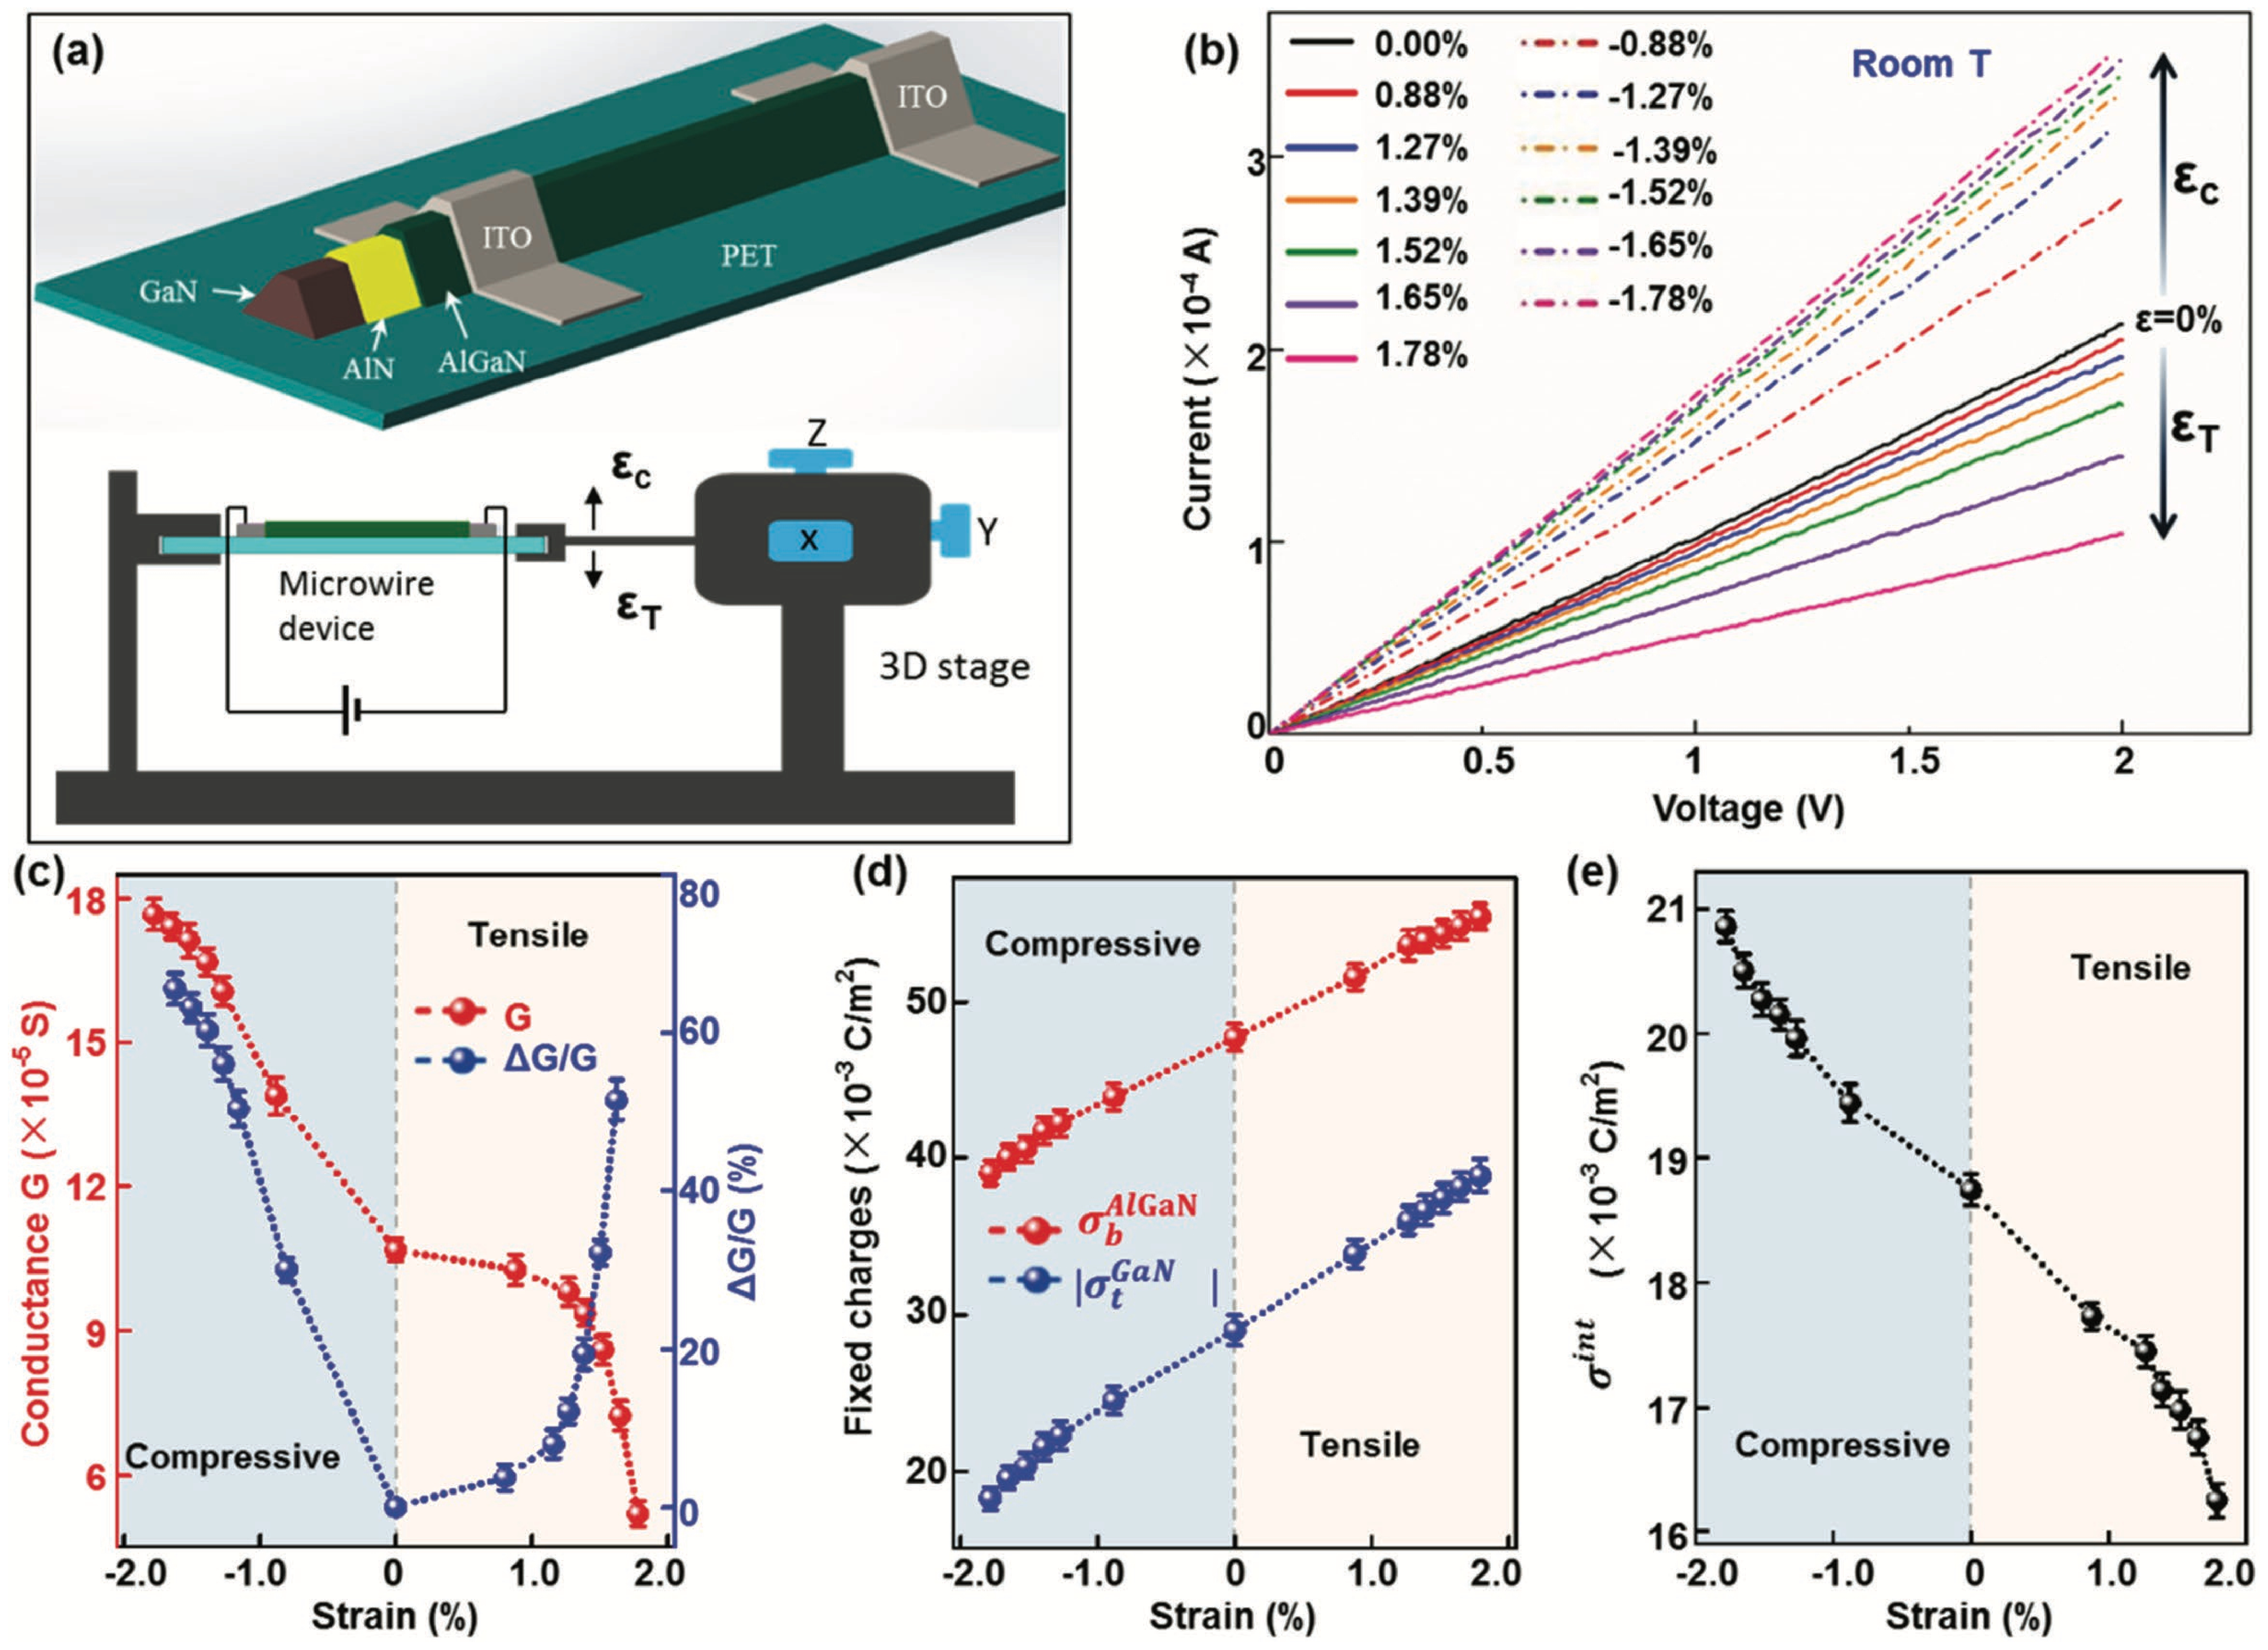
\includegraphics[width=0.9\textwidth]{ch1_9}
\caption[Piezotronic effect in AlGaN/AlN/GaN heterostructure microwire]{Piezotronic effect in AlGaN/AlN/GaN heterostructure microwire \protect\cite{wang2016piezotronic}}
\label{fig:1.9}
\end{figure}

In the work of Liu et al., the piezotronics effect in AlGaN/GaN MOS high-electron mobility-transistors (HEMT) \cite{liu2017electrical,Liu2018flexible} was studied for the first time (\autoref{fig:1.10}). Traditional AlGaN/GaN MOS HEMTs adjust the 2DEG concentration \index{Two-dimensional electron gas (2DEG)} at the interface \index{Interface} by adjusting the alloy composition or modifying the thickness of the epitaxial \index{Epitaxial!layer} layer, which modulates \index{Modulation} the electrical properties of the HEMT \index{HEMT} device mainly from the perspective of materials science. This work is the first to use strain-induced \index{Strain} piezoelectric polarization charge \index{Piezoelectric!polarization charge} to change the energy band \index{Energy band} distribution in AlGaN/GaN heterojunctions, thereby affecting the carrier distribution \index{Carrier!distribution} and 2DEG concentration \index{Two-dimensional electron gas (2DEG)} and modulating the electrical properties of HEMT devices. This study deepens the understanding of piezotronics \index{Piezotronics} effects in AlGaN/GaN heterojunction transistors and provides a new idea for the research of piezotronics \index{Piezotronics} transistors based on AlGaN/GaN HEMTs.

\begin{figure}[H] 
\centering    
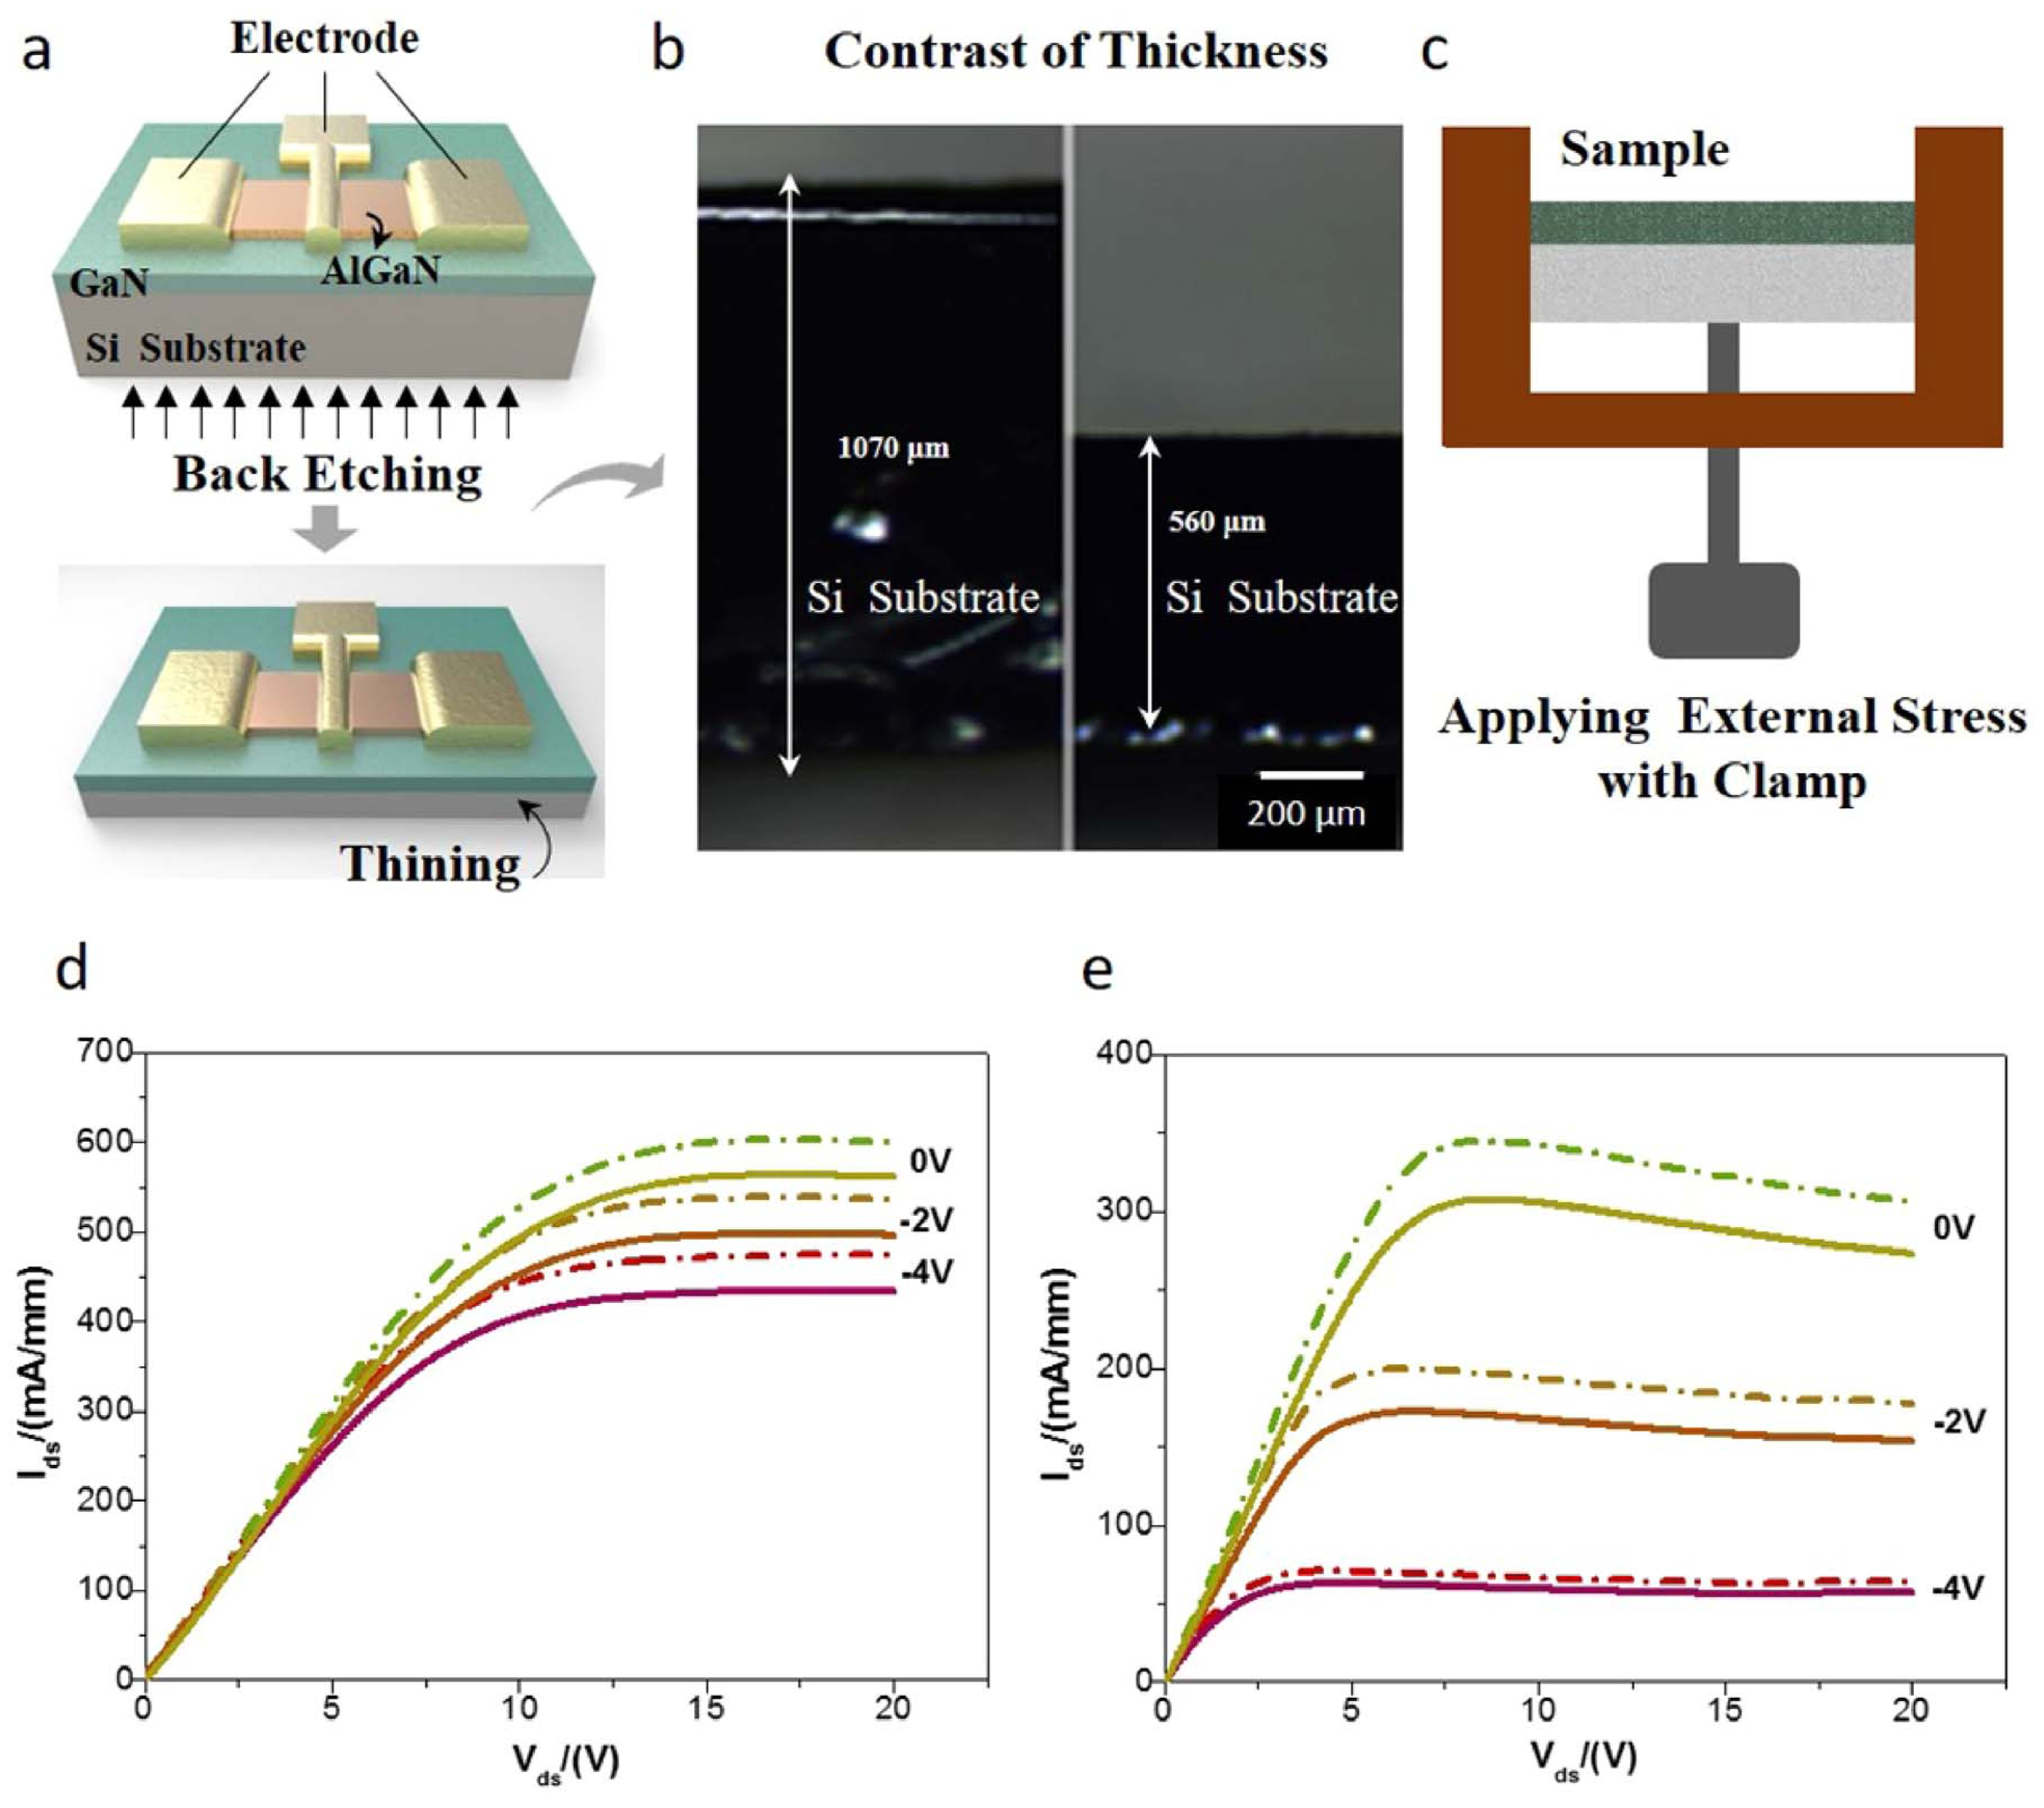
\includegraphics[width=0.9\textwidth]{ch1_10}
\caption[Piezotronics effect in AlGaN/GaN MOS HEMTs and unpassivated HEMTs]{Piezotronics effect in AlGaN/GaN MOS HEMTs and unpassivated HEMTs \protect\cite{liu2017electrical}}
\label{fig:1.10}
\end{figure}

Flexible electronics have received increasing attention due to their wide-ranging applications in fields such as healthcare, robotics, and artificial intelligence. Based on the work of Liu et al., Zhu et al. successfully fabricated flexible AlGaN/GaN HEMTs \index{HEMT} and studied their electrical properties under bending strain \index{Strain} through piezotronics \index{Piezotronics} effects (\autoref{fig:1.11}) \cite{zhu2019piezotronic,zhu2020thesis}. 

\begin{figure}[H] 
\centering    
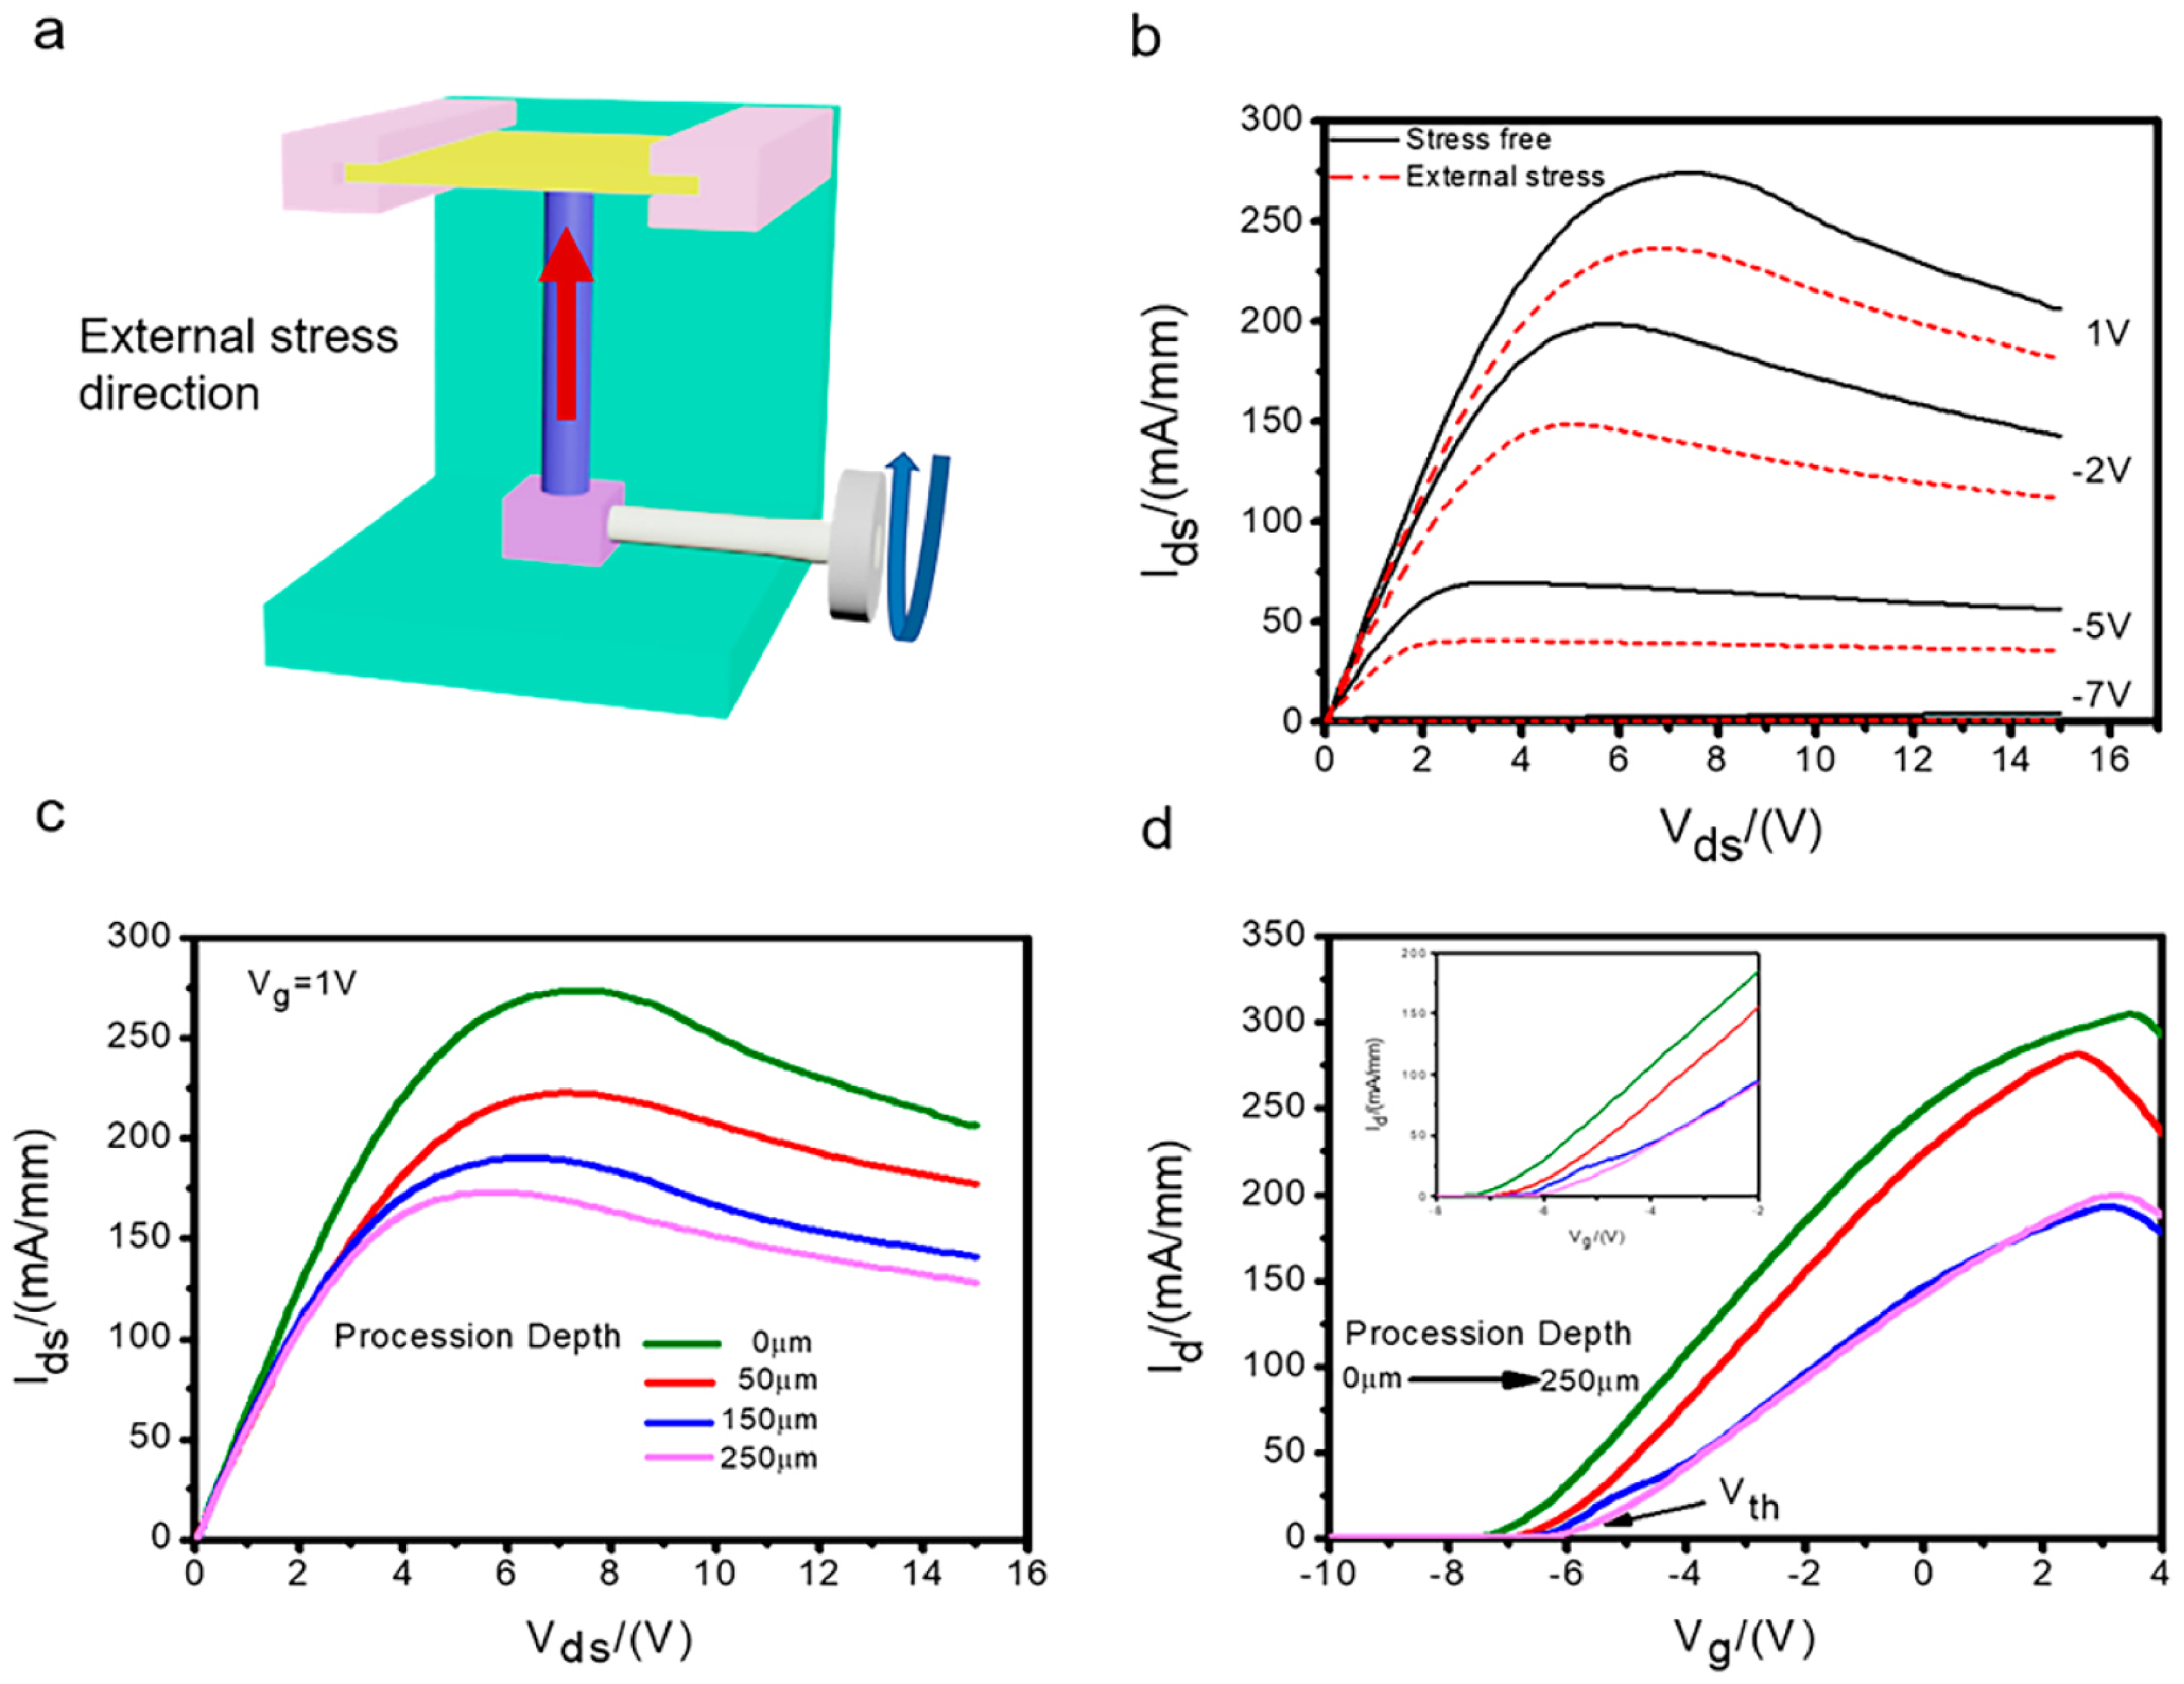
\includegraphics[width=0.9\textwidth]{ch1_11}
\caption[Piezotronics effect modulated flexible AlGaN/GaN HEMT]{Piezotronics effect modulated flexible AlGaN/GaN HEMT \protect\cite{zhu2019piezotronic}}
\label{fig:1.11}
\end{figure}

\noindent The fabricated flexible AlGaN/GaN HEMT \index{HEMT} completely removes the rigid silicon substrate \index{Substrate} and has excellent electrical properties. When the gate voltage \index{Voltage!gate voltage} $V_{gs}$ = \SI{2}{\volt}, the maximum saturated drain current \index{Current!drain current} density $I_{ds,max}$ reaches 290 \unit{\mA\per\mm}, The maximum transconductance \index{Transconductance} $g_{m, max}$ reaches 40 \unit{\milli\siemens\per\mm}. At the same time, the flexible HEMT can withstand large bending \index{Strain} strains. Based on the piezotronics \index{Piezotronics} effect of the AlGaN/GaN heterojunction, mechanical stress was introduced in the experiment to study the electrical properties of the flexible HEMT under strain. The results show that the output current \index{Output!current} of the flexible HEMT \index{HEMT} device can be significantly modulated \index{Modulation} by the external strain, and the electrical performance of the device will be degraded \index{Degradation} if it is subjected to forward bending \index{Strain} strain. Flexible HEMT devices modulated by piezotronics effects \index{Piezotronics} have broad application prospects in the fields of wearable electronics, smart \index{MEMS} MEMS, and human-computer interaction.


%********************************** % Third Section  *************************************
\section{Introduction to III-V nitride MEMS devices}  %Section - 1.3 

\subsection{Introduction to micro-electromechanical systems (MEMS)}

In the past decade, Micro-electromechanical systems (MEMS) \index{MEMS} technology has developed from a basic exploratory research to an important mainstream technology that has been widely used in many fields \cite{lyshevski2018nano,hsumems,gardner2003microsensors}. As an industrial technology that integrates microelectronics technology and mechanical engineering, MEMS combines the electrical information processing function and the mechanical sensing function to form a micro-electromechanical integrated system. MEMS have three main characteristics:

\begin{itemize}
	\item [1)] Combines electrical and mechanical components in order to sense its environment (mechanical sensors).
	\item [2)] Ability to analyze data (electronics) and react to changes in the environment (actuators).
	\item [3)] Devices are typically fabricated by microelectronics and have dimensions on the order of micrometers to millimeters.
\end{itemize}

Therefore, MEMS can "perceive", "think" and "react", and it is an intelligent micro-integrated system. The system block diagram of MEMS is shown in \autoref{fig:1.12}.

\begin{figure}[H] 
\centering    
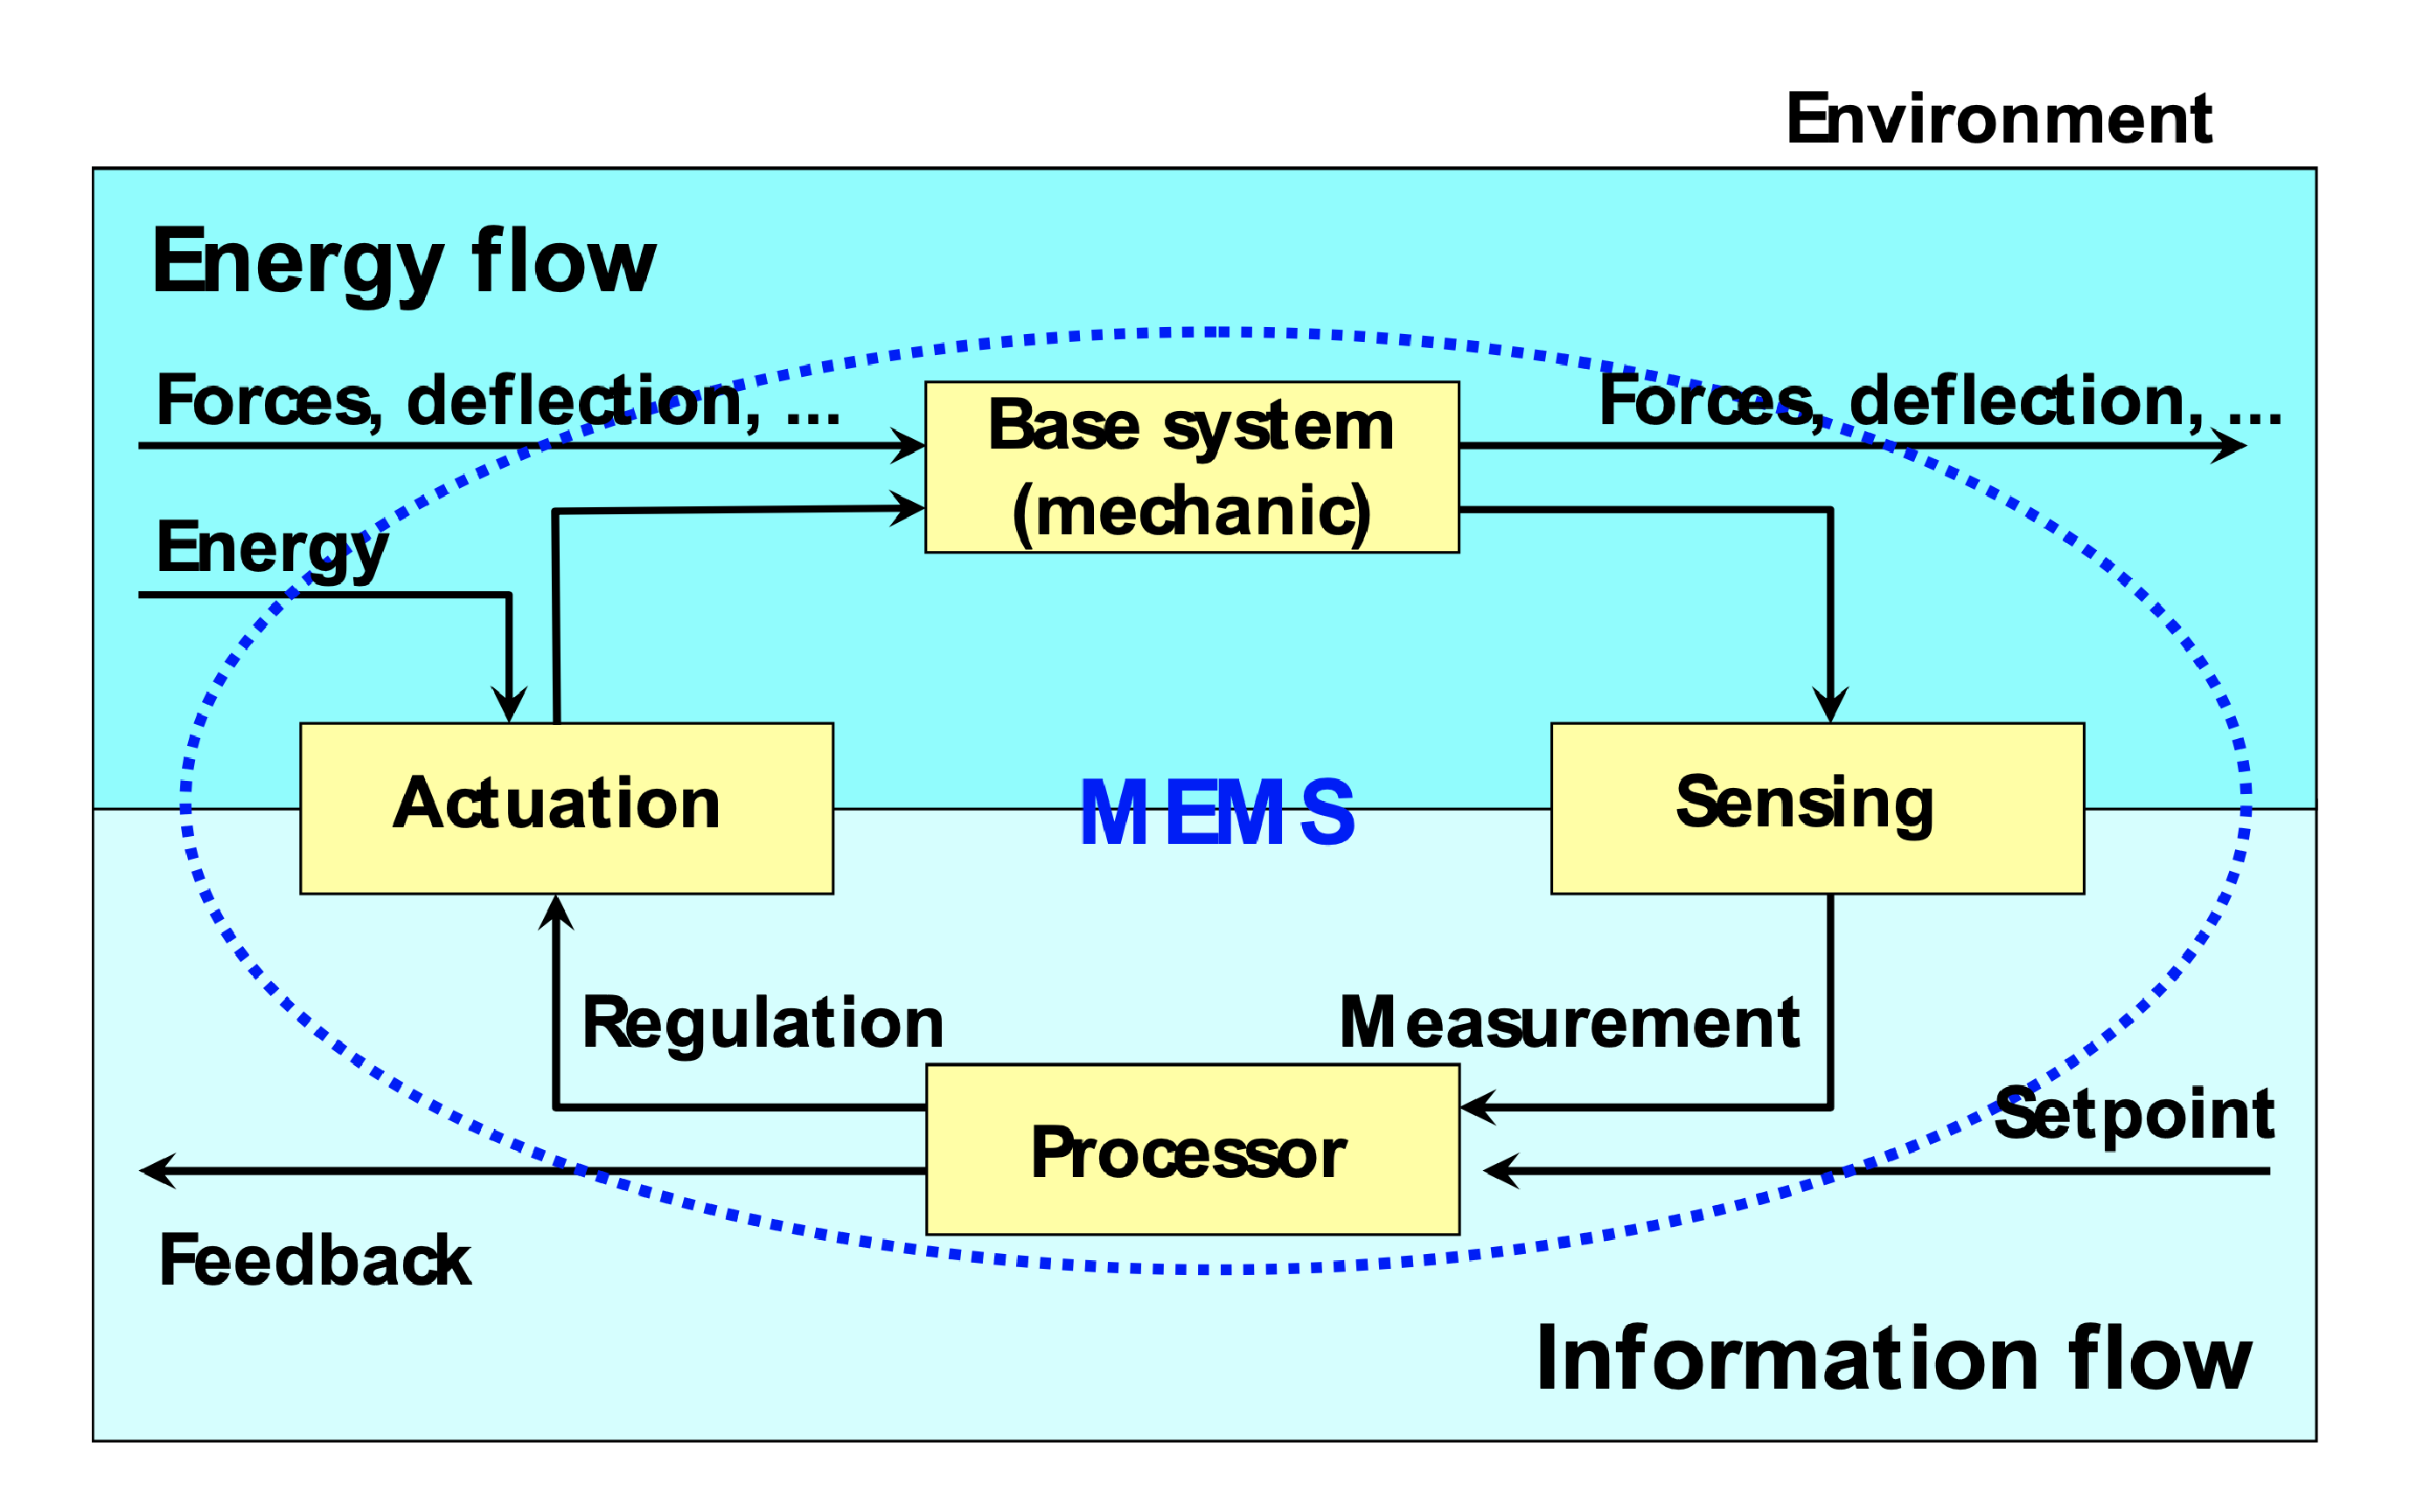
\includegraphics[width=0.9\textwidth]{ch1_12}
\caption[Block diagram for the basic components in MEMS and their interaction]{Block diagram for the basic components in MEMS and their interaction \protect\cite{cimalla2010algan}}
\label{fig:1.12}
\end{figure}


\subsection{III-V nitride MEMS devices}

With the rapid development of silicon-based microelectronics technology, the integration of Si-based MEMS \index{MEMS} devices has rapidly increased, and the system's "response" is faster, more reliable, cheaper, and capable of incorporating more complex functions. Si-based MEMS devices are being used in more and more fields \cite{ciuti2015mems}, including chemical, biological and physical sensors \cite{yabuki2014heat,wang2004ultra,khoshnoud2012recent-a,khoshnoud2012recent-b}, microfluidic sensors \cite{kottapalli2011liquid}, radio frequency MEMS \cite{fernandez2006capacitive,donelli2018exploitation}, micro-opto-electro-mechanical system (MOEMS) \cite{lee2008development,iannacci2018internet}, Internet of Things, etc., as well as various MEMS-based acceleration, pressure, and flow sensors \cite{davidson2008using,marek2011automotive,berndt2020mems} used in the automotive industry. However, Si-based MEMS have shown limitations for sensing in harsh environmental conditions \cite{french2016precision}, an issue that has received increasing attention over the past few years. First, Si-based MEMS cannot be used for high-temperature applications because Si materials lose mechanical reliability at \SI{500}{\degreeCelsius} \cite{french2016precision}. Second, Si materials are easily attacked by corrosive media and have low biochemical compatibility, which limits its application in the field of biosensing \cite{french2016precision}. Therefore, additional protection of the sensing and actuation elements is necessary for chemical and biological Si-based MEMS sensors, which are generally no longer integrated systems. For these reasons, Si-based MEMS allow only very limited applications. These shortcomings of Si-based MEMS technology have stimulated research into MEMS of more biochemically resistant and thermally stable materials such as wide-bandgap semiconductors.

\begin{table}[H]
\renewcommand\arraystretch{1.2}
\centering
\caption[Comparison of characteristics of several electromechanical materials]{Comparison of characteristics of several electromechanical materials \protect\cite{rais2014gallium}}
\begin{tabular}{ccccccc}
\hline
\hline
Material &
  \begin{tabular}[c]{@{}c@{}}Elastic \\Modulus $C33$ \\ (\unit{GPa})\end{tabular} &
  \begin{tabular}[c]{@{}c@{}}Acoustic \\Velocity\\  (\unit{m/s})\end{tabular} &
  \begin{tabular}[c]{@{}c@{}}Piezoelectric \\Coefficient $e33$ \\ (\unit{\coulomb\per\square\m})\end{tabular} &
  \begin{tabular}[c]{@{}c@{}}$f \times Q$ \\ (\unit{Hz}) \end{tabular} &
  \begin{tabular}[c]{@{}c@{}}$K_{eff}^{2}$ \\ (\%) \end{tabular} &
  Ref \\ \hline \hline
Si   & 165 & 8415  & N/A   & \num{2.5e13}   & N/A  & \cite{tabrizian2009effect}       \\
SiC  & 605 & 13100 & 0.2   & \num{3.5e14}   & 0.08 & \cite{tabrizian2009effect,karmann1989piezoelectric,shur1996handbook,shur2006sic}    \\
GaAs & 118 & 2470  & -0.16 & --                     & 0.04 & \cite{adachi1992physical,adachi1994gaas}    \\
AlN  & 390 & 11000 & 1.55  & \num{e13}              & 5.6  & \cite{tabrizian2009effect,zou2010high}    \\
GaN  & 398 & 8044  & 0.65  & \num{5.0e12}     & 2    & \cite{tabrizian2009effect,gokhale2014phonon,gokhale2010observation,gokhale2011high,popa2014band} \\ \hline \hline
\end{tabular}
\label{tab:1.1}
\end{table}

III-V nitride \index{Nitride} materials are the main representatives of wide-bandgap semiconductors because of unique material properties that exhibit excellent mechanical, electrical, and perceptual properties in \index{MEMS} MEMS applications (\autoref{fig:1.13}) \cite{rais2014gallium,strittmatter2004development,cimalla2007group}. Compared to Si \cite{ekinci2005nanoelectromechanical}, the high Young's modulus \index{Young's modulus} of III-V nitrides \index{Nitride} enables higher frequencies and quality factor in resonant devices of the same geometry (\autoref{tab:1.1}). In addition, materials with high Young's modulus can better maintain the linear relationship between applied load and induced \index{Strain} strain. Another major advantage of III-V nitrides is their very high mechanical, thermal, chemical and biological stability \cite{kuball1998thermal,cimalla2007algan}. They have no or very low reactivity with molecules in air, and can be applied in reliable environmental sensors. Therefore, III-V nitride materials are very suitable for MEMS \index{MEMS} or NEMS applications. Finally, due to the high frequency properties of III-V nitride materials, they can be combined or integrated into MEMS as amplifiers for radio frequency devices. It is worth mentioning that the piezoelectric effect \index{Piezoelectric!effect} offers completely new possibilities to integrate new functionalities into MEMS devices \cite{tadigadapa2009piezoelectric}. The AlGaN/GaN heterojunction interface \index{Interface} contains a high concentration of two-dimensional \index{Two-dimensional electron gas (2DEG)} electron gas (2DEG), which is extremely sensitive to both mechanical loading and chemical modifications of the surface, such as (i) the charge on the free, unpassivated gate \index{Surface} surface; (ii) mechanical stress that modulates \index{Modulation} the internal piezoelectric \index{Piezoelectric!potential} potential; and (iii) external fields such as magnetic fields \index{Magnetic!field} or electromagnetic radiation. Therefore it is widely used in biochemical sensors \cite{eickhoff2003electronics,pearton2004gan,chen2008low,chang2008co,guo2012ph,kang2005electrical,kokawa2006liquid}, pressure sensors \cite{kang2005capacitance,sun2020low}, cantilever \index{Cantilever} sensors \cite{zimmermann2006piezoelectric,khmyrova2009multi,vittoz2011analytical}, and many other novel sensors. Compared with Si-based MEMS, MEMS \index{MEMS} devices based on III-V nitrides \index{Nitride} have broader development prospects.

\begin{figure}[H] 
\centering    
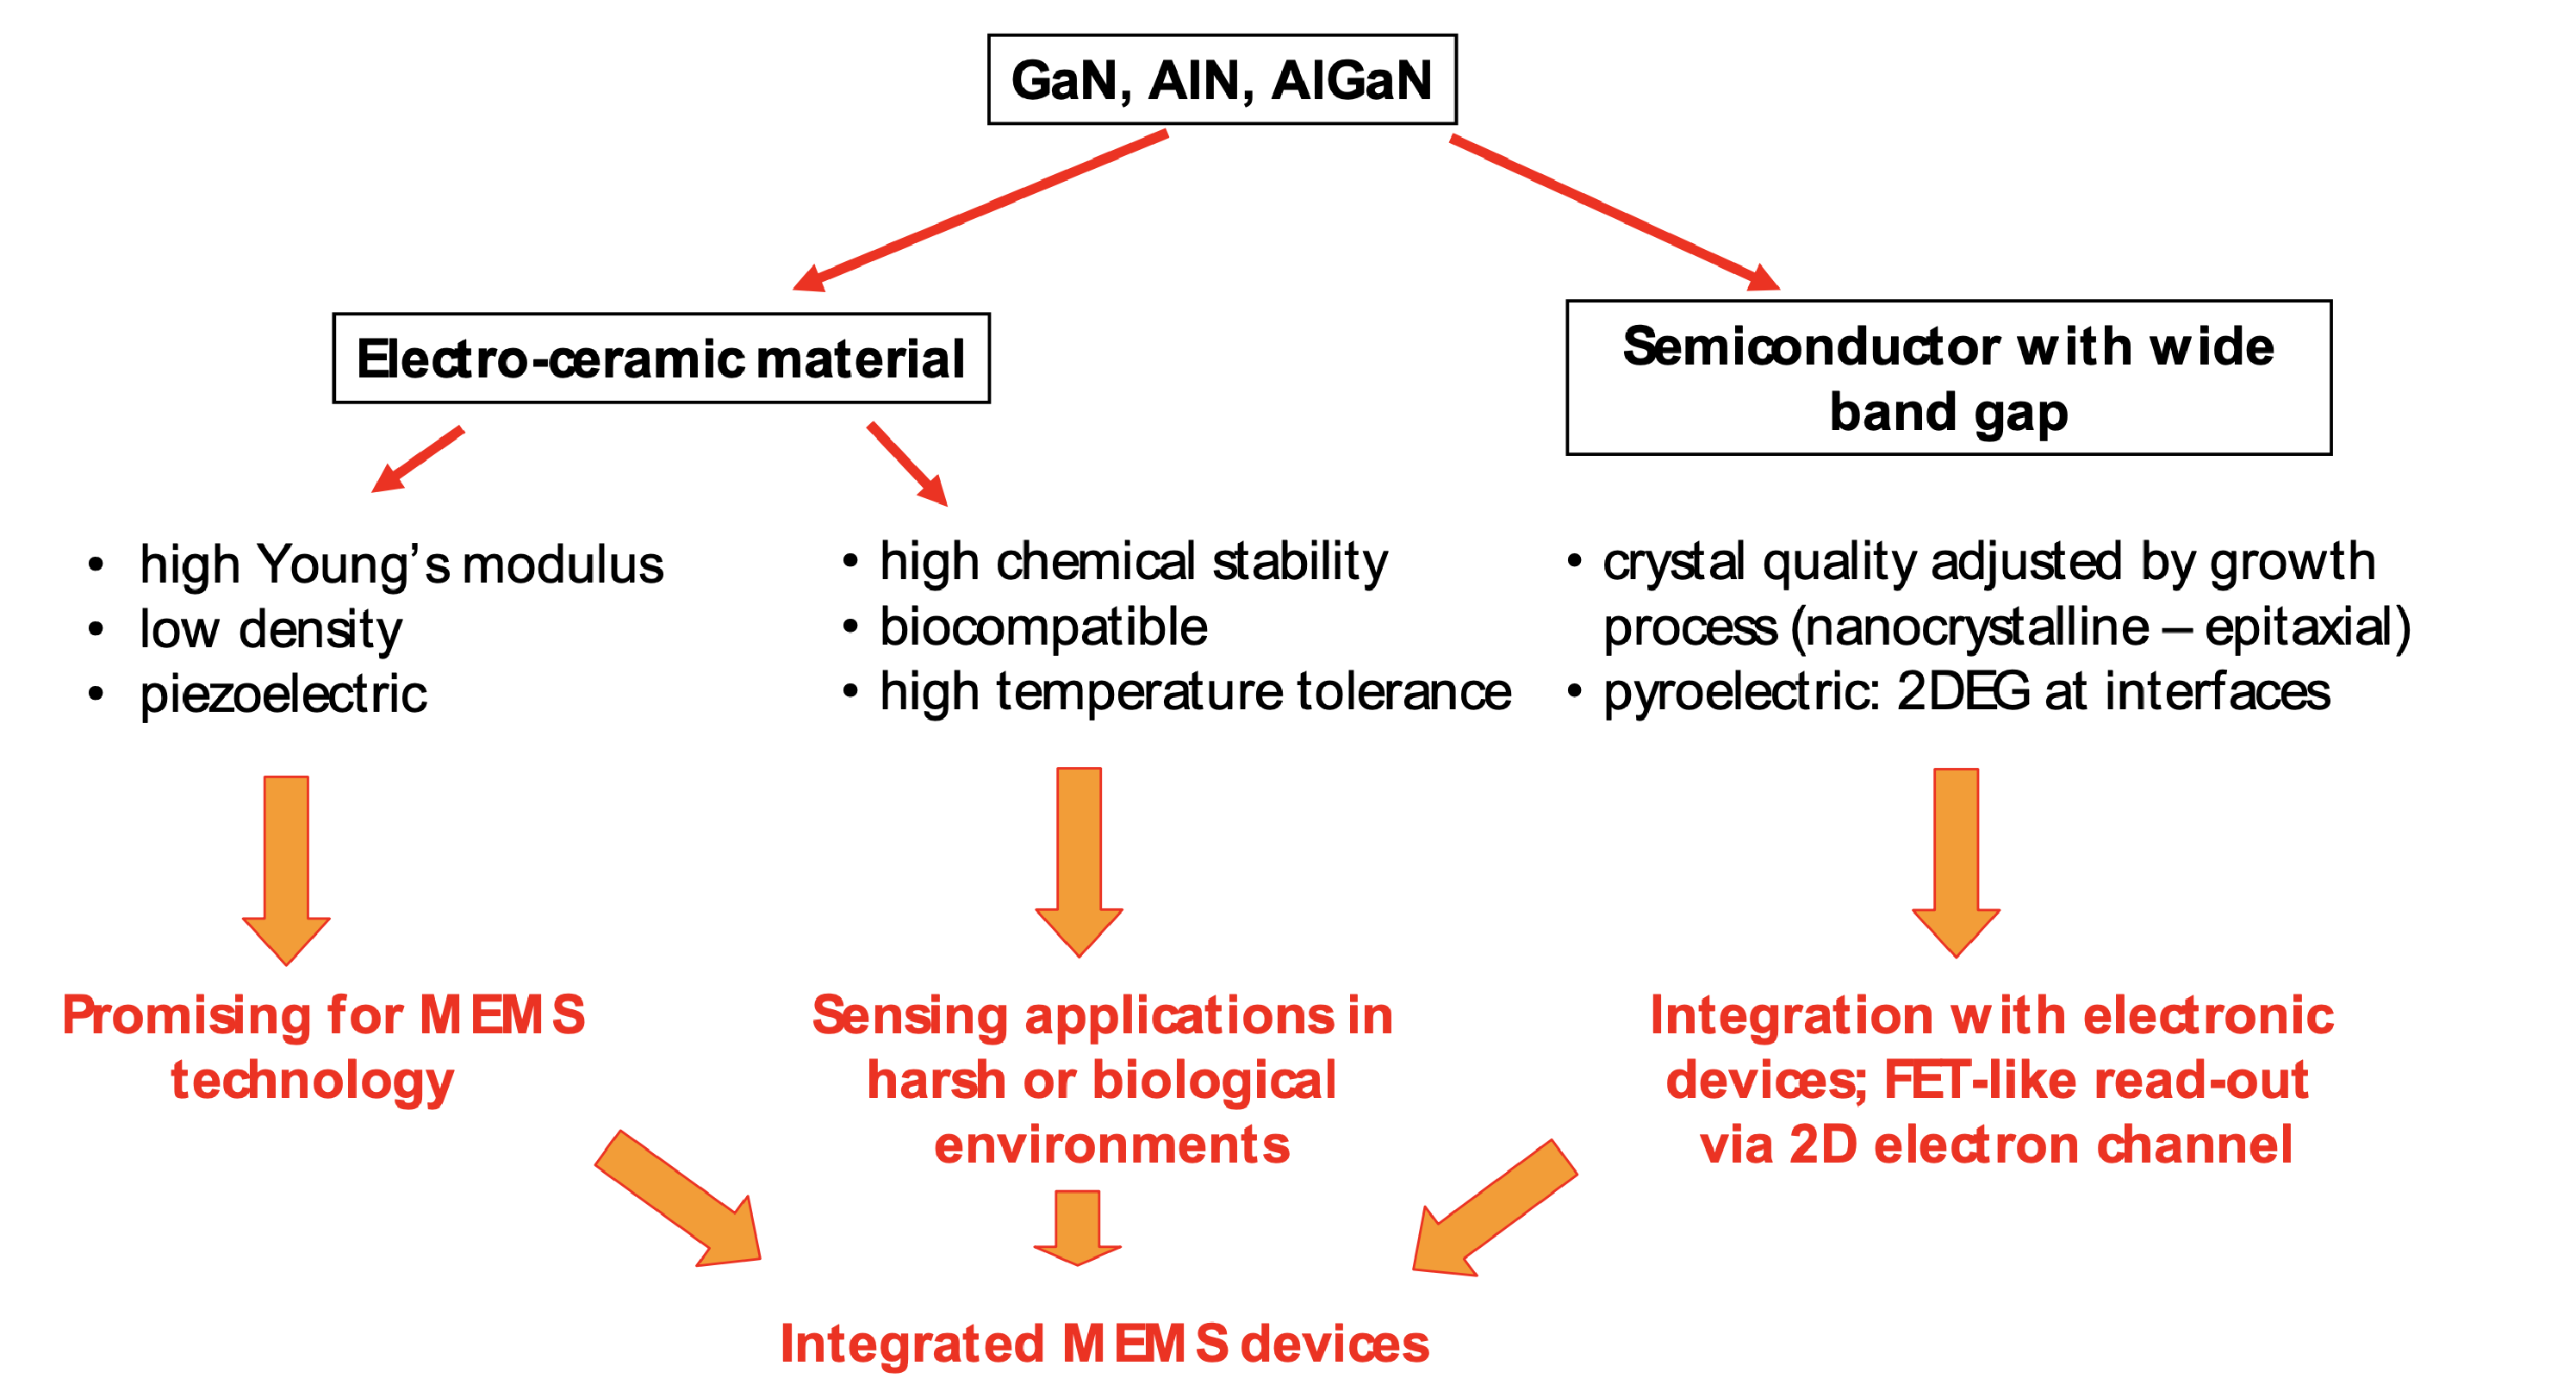
\includegraphics[width=0.9\textwidth]{ch1_13}
\caption[Advantages of group III-V nitrides for the realization of integrated MEMS]{Advantages of group III-V nitrides for the realization of integrated MEMS \protect\cite{cimalla2010algan}}
\label{fig:1.13}
\end{figure}

Based on the excellent properties of III-V nitride \index{Nitride} materials, the research on GaN-based MEMS \index{MEMS} devices has made remarkable progress. Azadeh Ansari et al. reported a gigahertz AlGaN/GaN resonant body transistor (RBT) \index{Resonant body transistor (RBT)} in which mechanical resonance and electrical signals can be modulated \index{Modulation} simultaneously, as shown in \autoref{fig:1.14} \cite{ansari2014thickness}. An AlGaN layer with a thickness of 17.5 \unit{\nm} was used as the piezoelectric transducer layer, and the 2DEG \index{Two-dimensional electron gas (2DEG)} at the AlGaN/GaN interface \index{Interface} was used as the bottom electrode \index{Electrode} as well as the transistor conduction \index{Channel} channel. The strain \index{Strain} generated by the acoustic wave can effectively modulate the 2DEG concentration \index{Two-dimensional electron gas (2DEG)} of the \index{Channel} channel. A quality factor of 250 and an acoustic transconductance \index{Transconductance} of 25 \unit{\micro\siemens} are obtained at the resonant frequency of 4.23 \unit{\GHz}, resulting in excellent mechanical and electrical properties.

\begin{figure}[H] 
\centering    
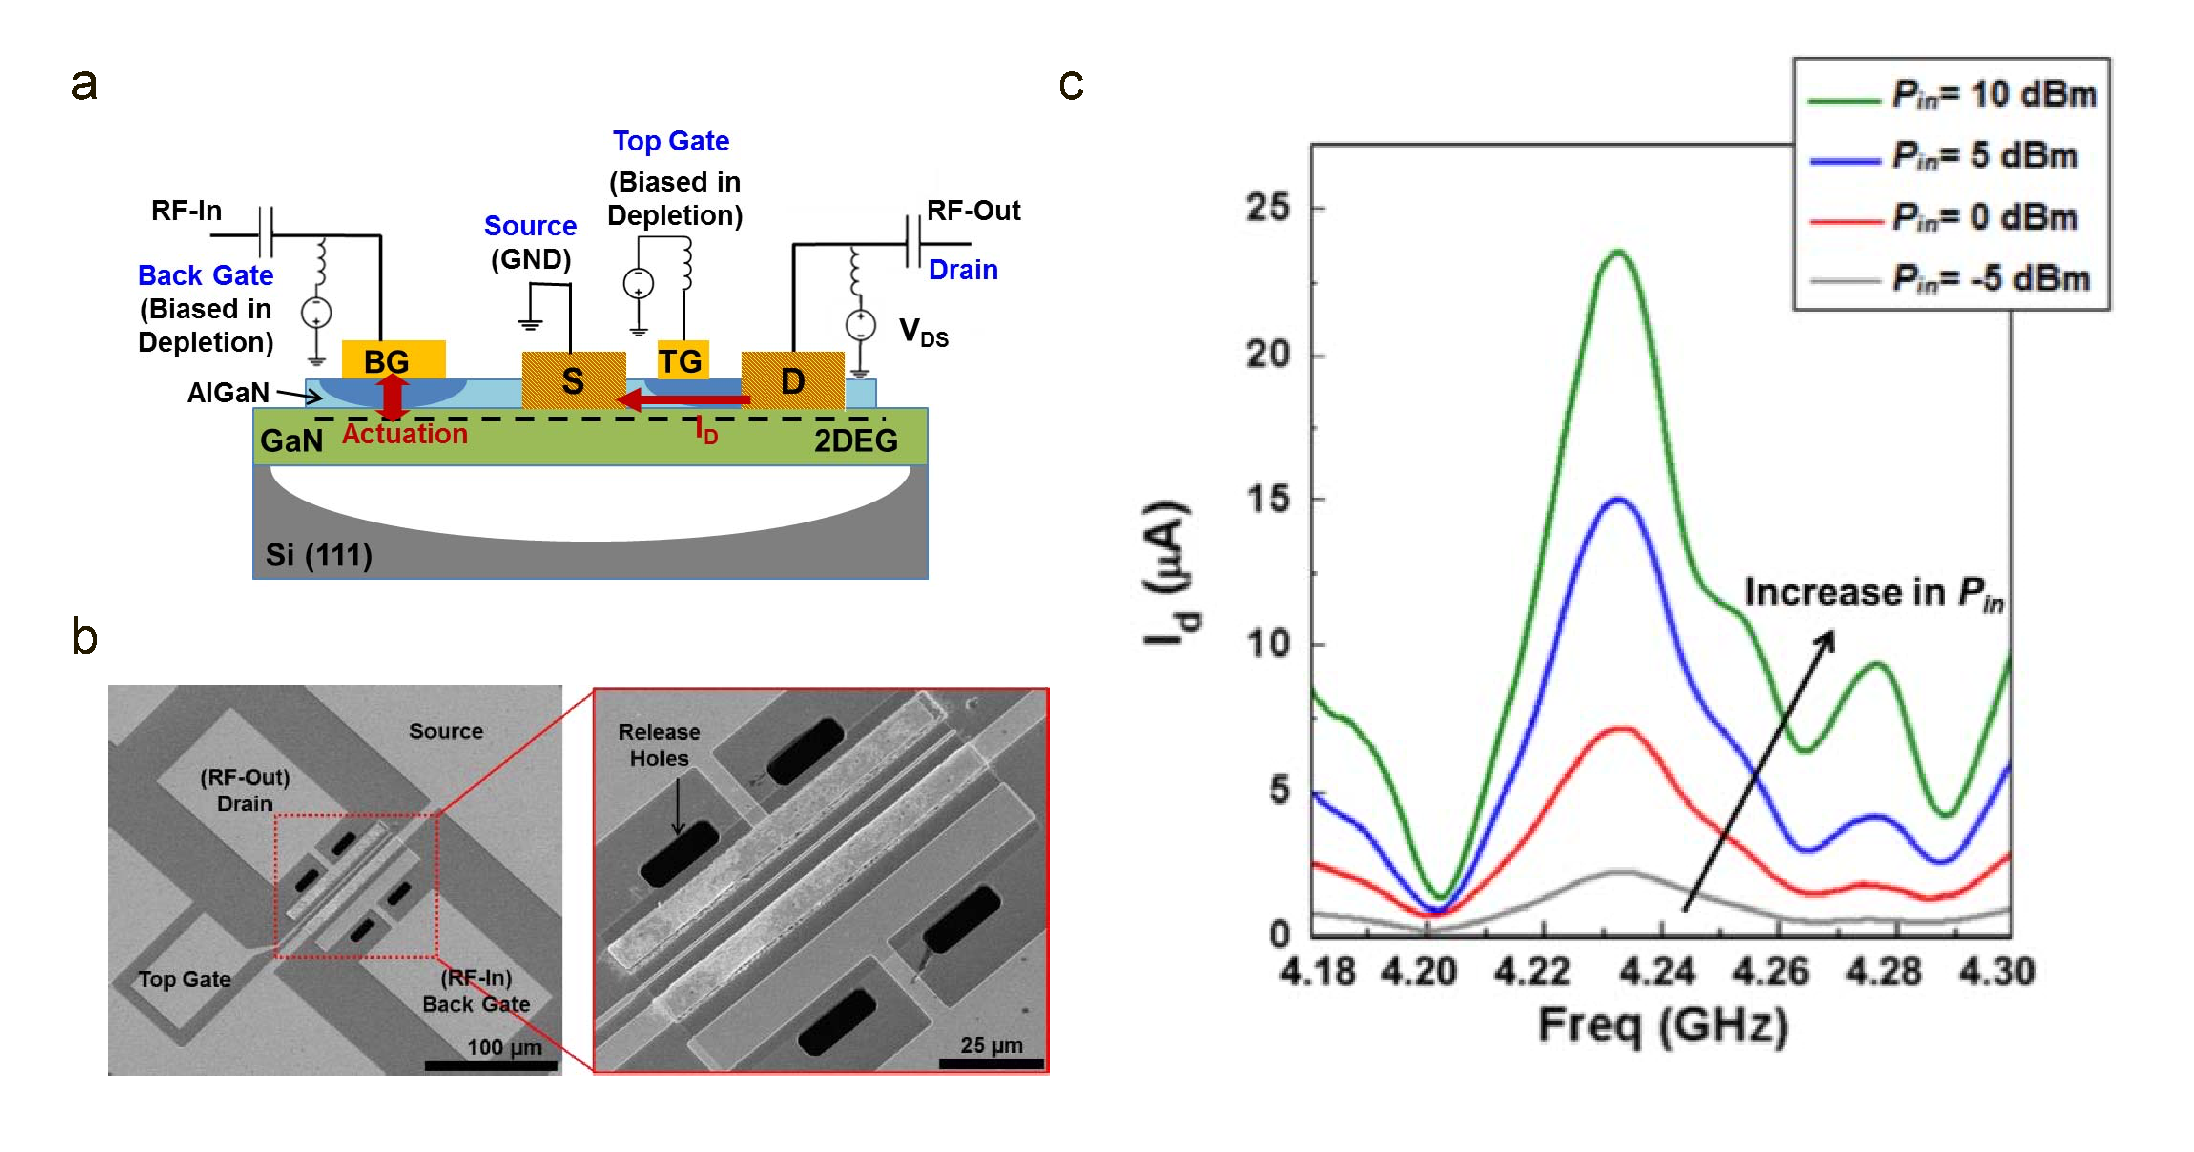
\includegraphics[width=0.9\textwidth]{ch1_14}
\caption[The AlGaN/GaN resonant body high electron mobility transistor]{The AlGaN/GaN resonant body high electron mobility transistor \protect\cite{ansari2014thickness}}
\label{fig:1.14}
\end{figure}

The development of all-GaN integrated \index{MEMS} MEMS has always been the focus of research in the field of GaN-based MEMS. On the basis of the above work, Azadeh Ansari et al. reported an all-GaN integrated microsystem platform integrating high-frequency GaN-based MEMS resonators and AlGaN/GaN HEMTs, as shown in \autoref{fig:1.15} \cite{ansari2012monolithic}. For the first time, stacked high-quality GaN bulk acoustic resonators and AlGaN/GaN \index{HEMT} HEMTs have been fabricated on \index{Substrate} silicon substrates, achieving signal tuning over 30 \unit{\dB} using HEMT \index{HEMT} amplifiers. This work can serve as a starting point for further development of integrated GaN-based MEMS, that is, integrating GaN-based devices (MEMS, HEMT, RBT, etc.) together to build fully GaN integrated MEMS with different architectures and functions.

\begin{figure}[H] 
\centering    
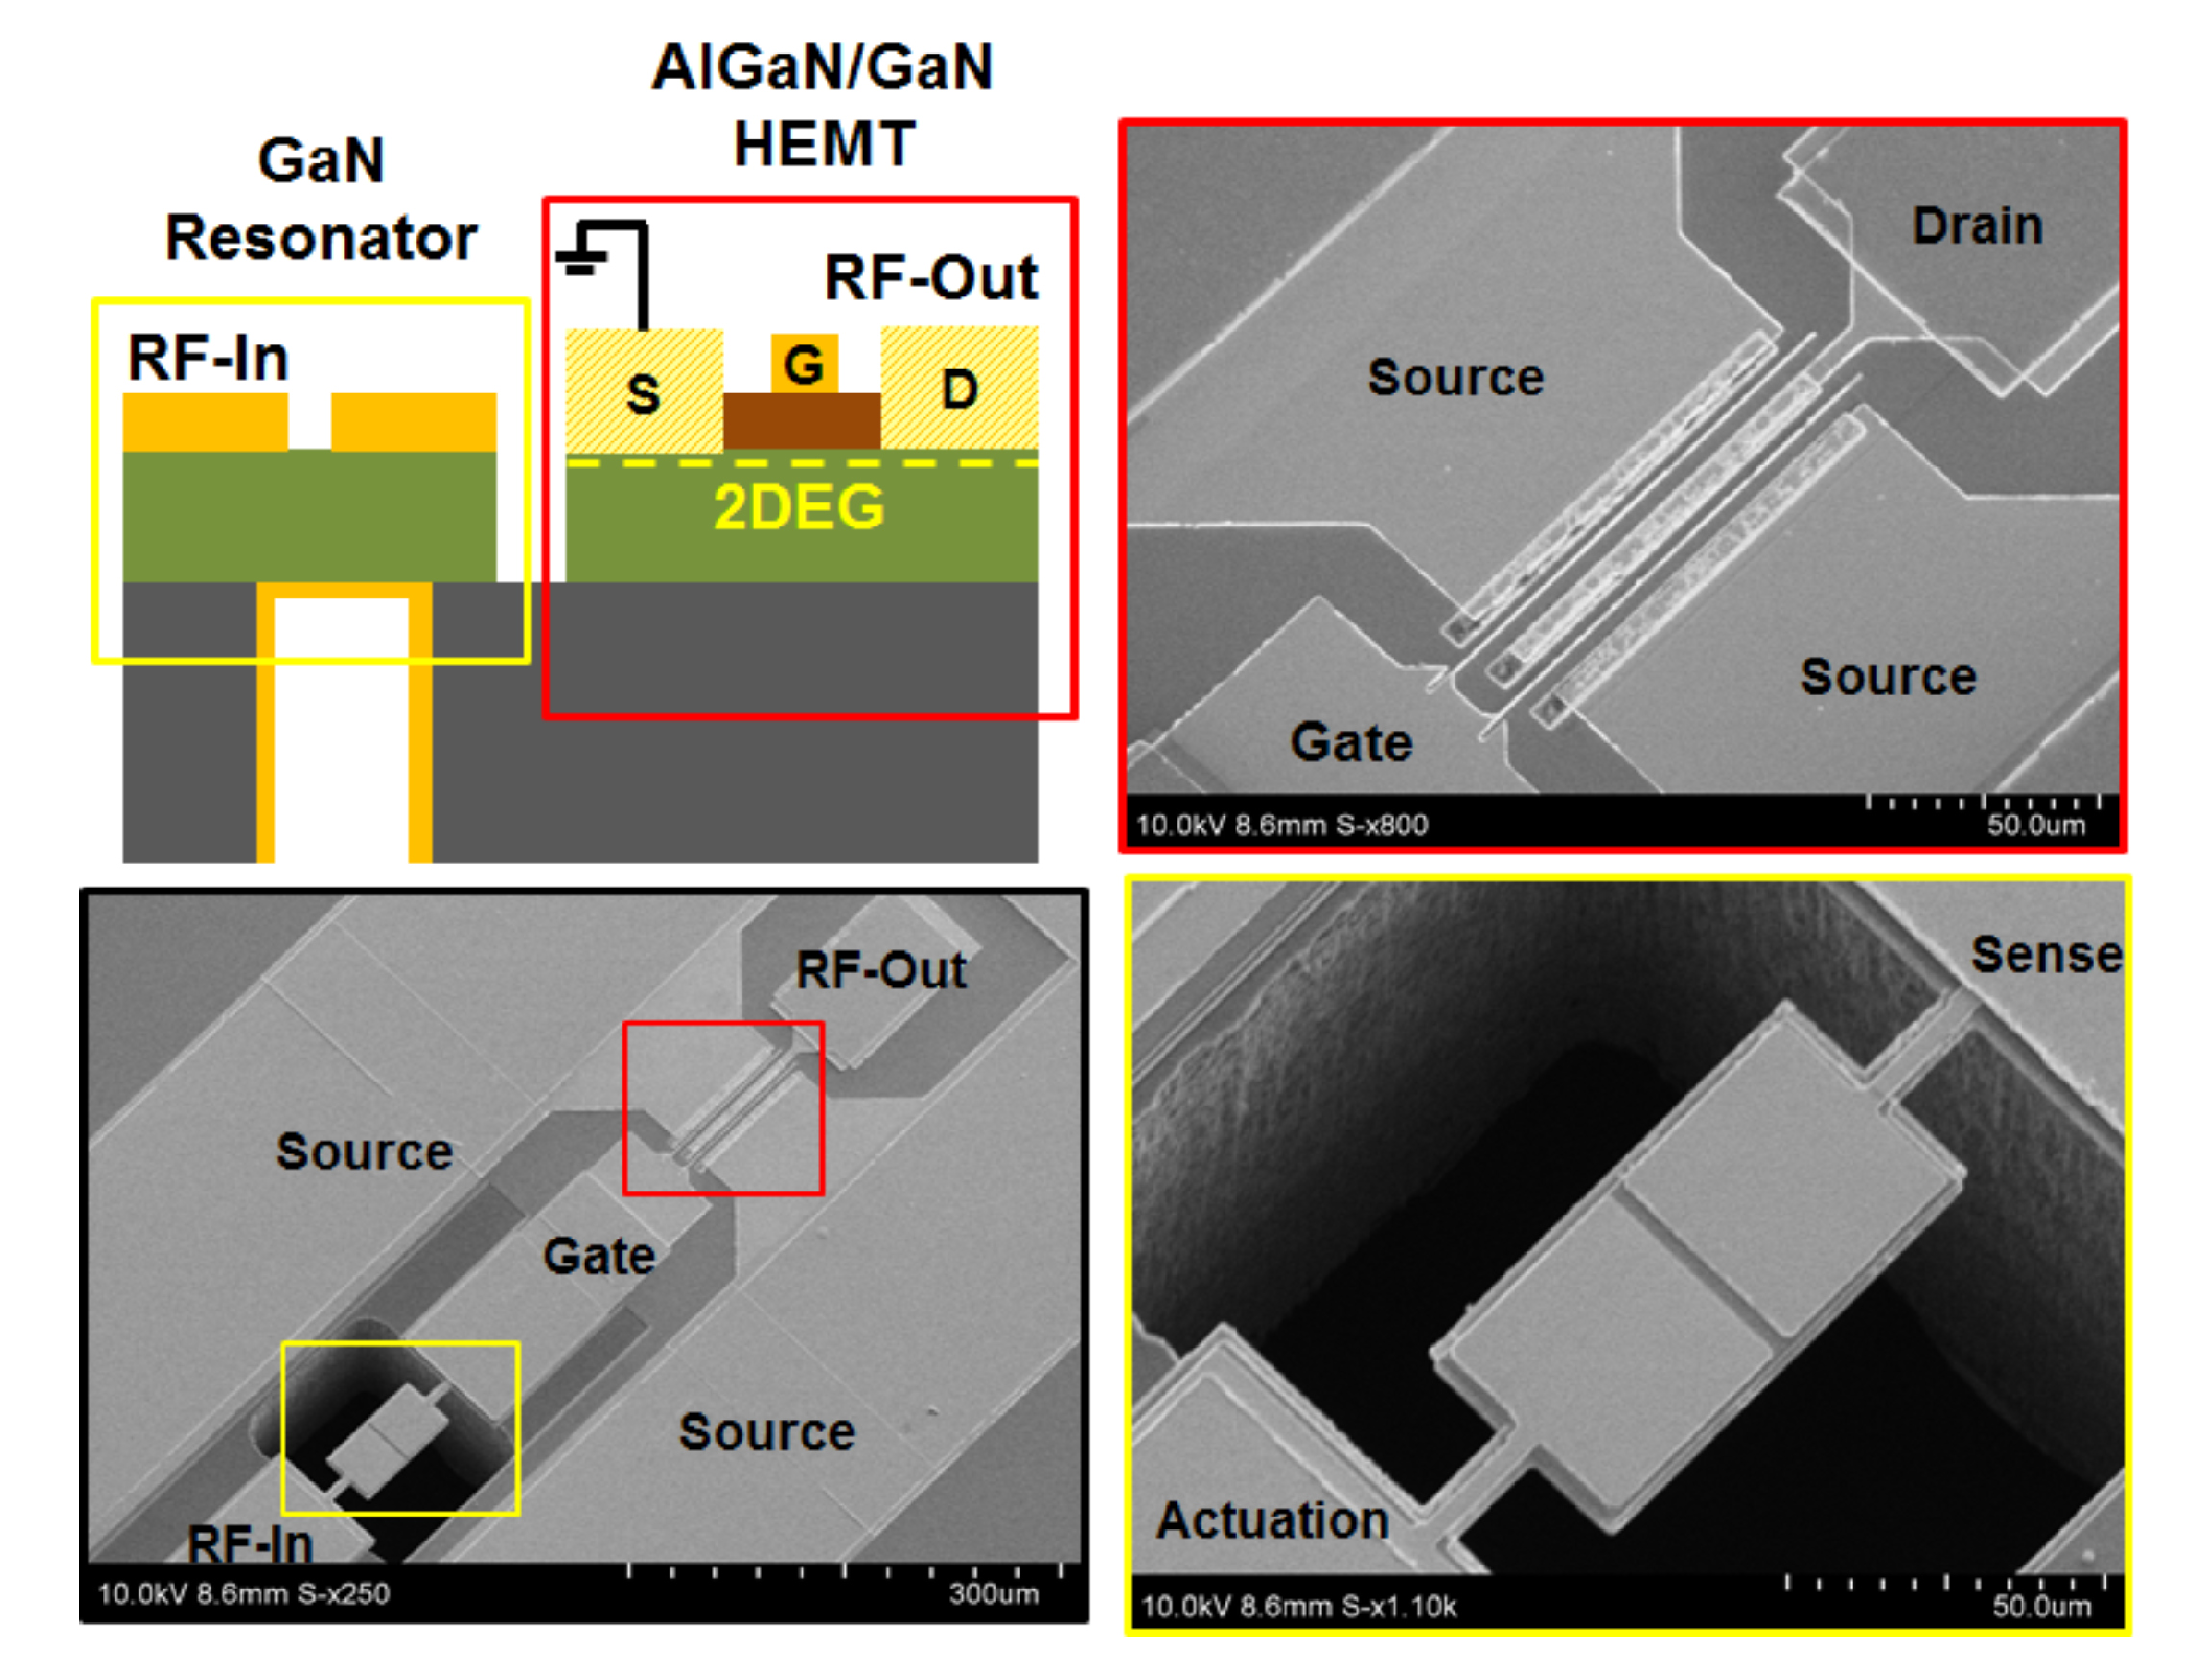
\includegraphics[width=0.9\textwidth]{ch1_15}
\caption[An all-GaN integrated microsystem platform wherein GaN MEMS resonators are monolithically integrated with AlGaN/GaN HEMT]{An all-GaN integrated microsystem platform wherein GaN MEMS resonators are monolithically integrated with AlGaN/GaN HEMT \protect\cite{ansari2012monolithic}}
\label{fig:1.15}
\end{figure}

Based on the unique piezoelectric effect \index{Piezoelectric!effect} of III-V nitride \index{Nitride} materials, Sun et al. reported a miniature pressure MEMS \index{MEMS} sensor based on a suspended structure of AlGaN/GaN heterojunction (\autoref{fig:1.16}) \cite{sun2020low}. The sensor's drain current \index{Current!drain current} can respond quickly when subjected to different pressures (especially in the low pressure range below 600 \unit{Pa}). Under the operating condition of \SI{100}{\degreeCelsius}, the dynamic current change percentage of the sensor is 18.75$\%$ when the pressure is changed from 96 \unit{KPa} to 10 \unit{Pa}, and the power consumption is only 1.8 \unit{uW}. In the pressure range of 600 \unit{Pa} to 10 \unit{Pa}, the maximum sensitivity of the sensor is 22.8$\%$/\unit{KPa}. Meanwhile, at higher temperature, the thermally induced displacement of the film increases the 2DEG \index{Two-dimensional electron gas (2DEG)} concentration, and the drain current response of the sensor increases accordingly. Therefore, miniature pressure MEMS sensors can be applied to high vacuum and high temperature sensing.

\begin{figure}[H] 
\centering    
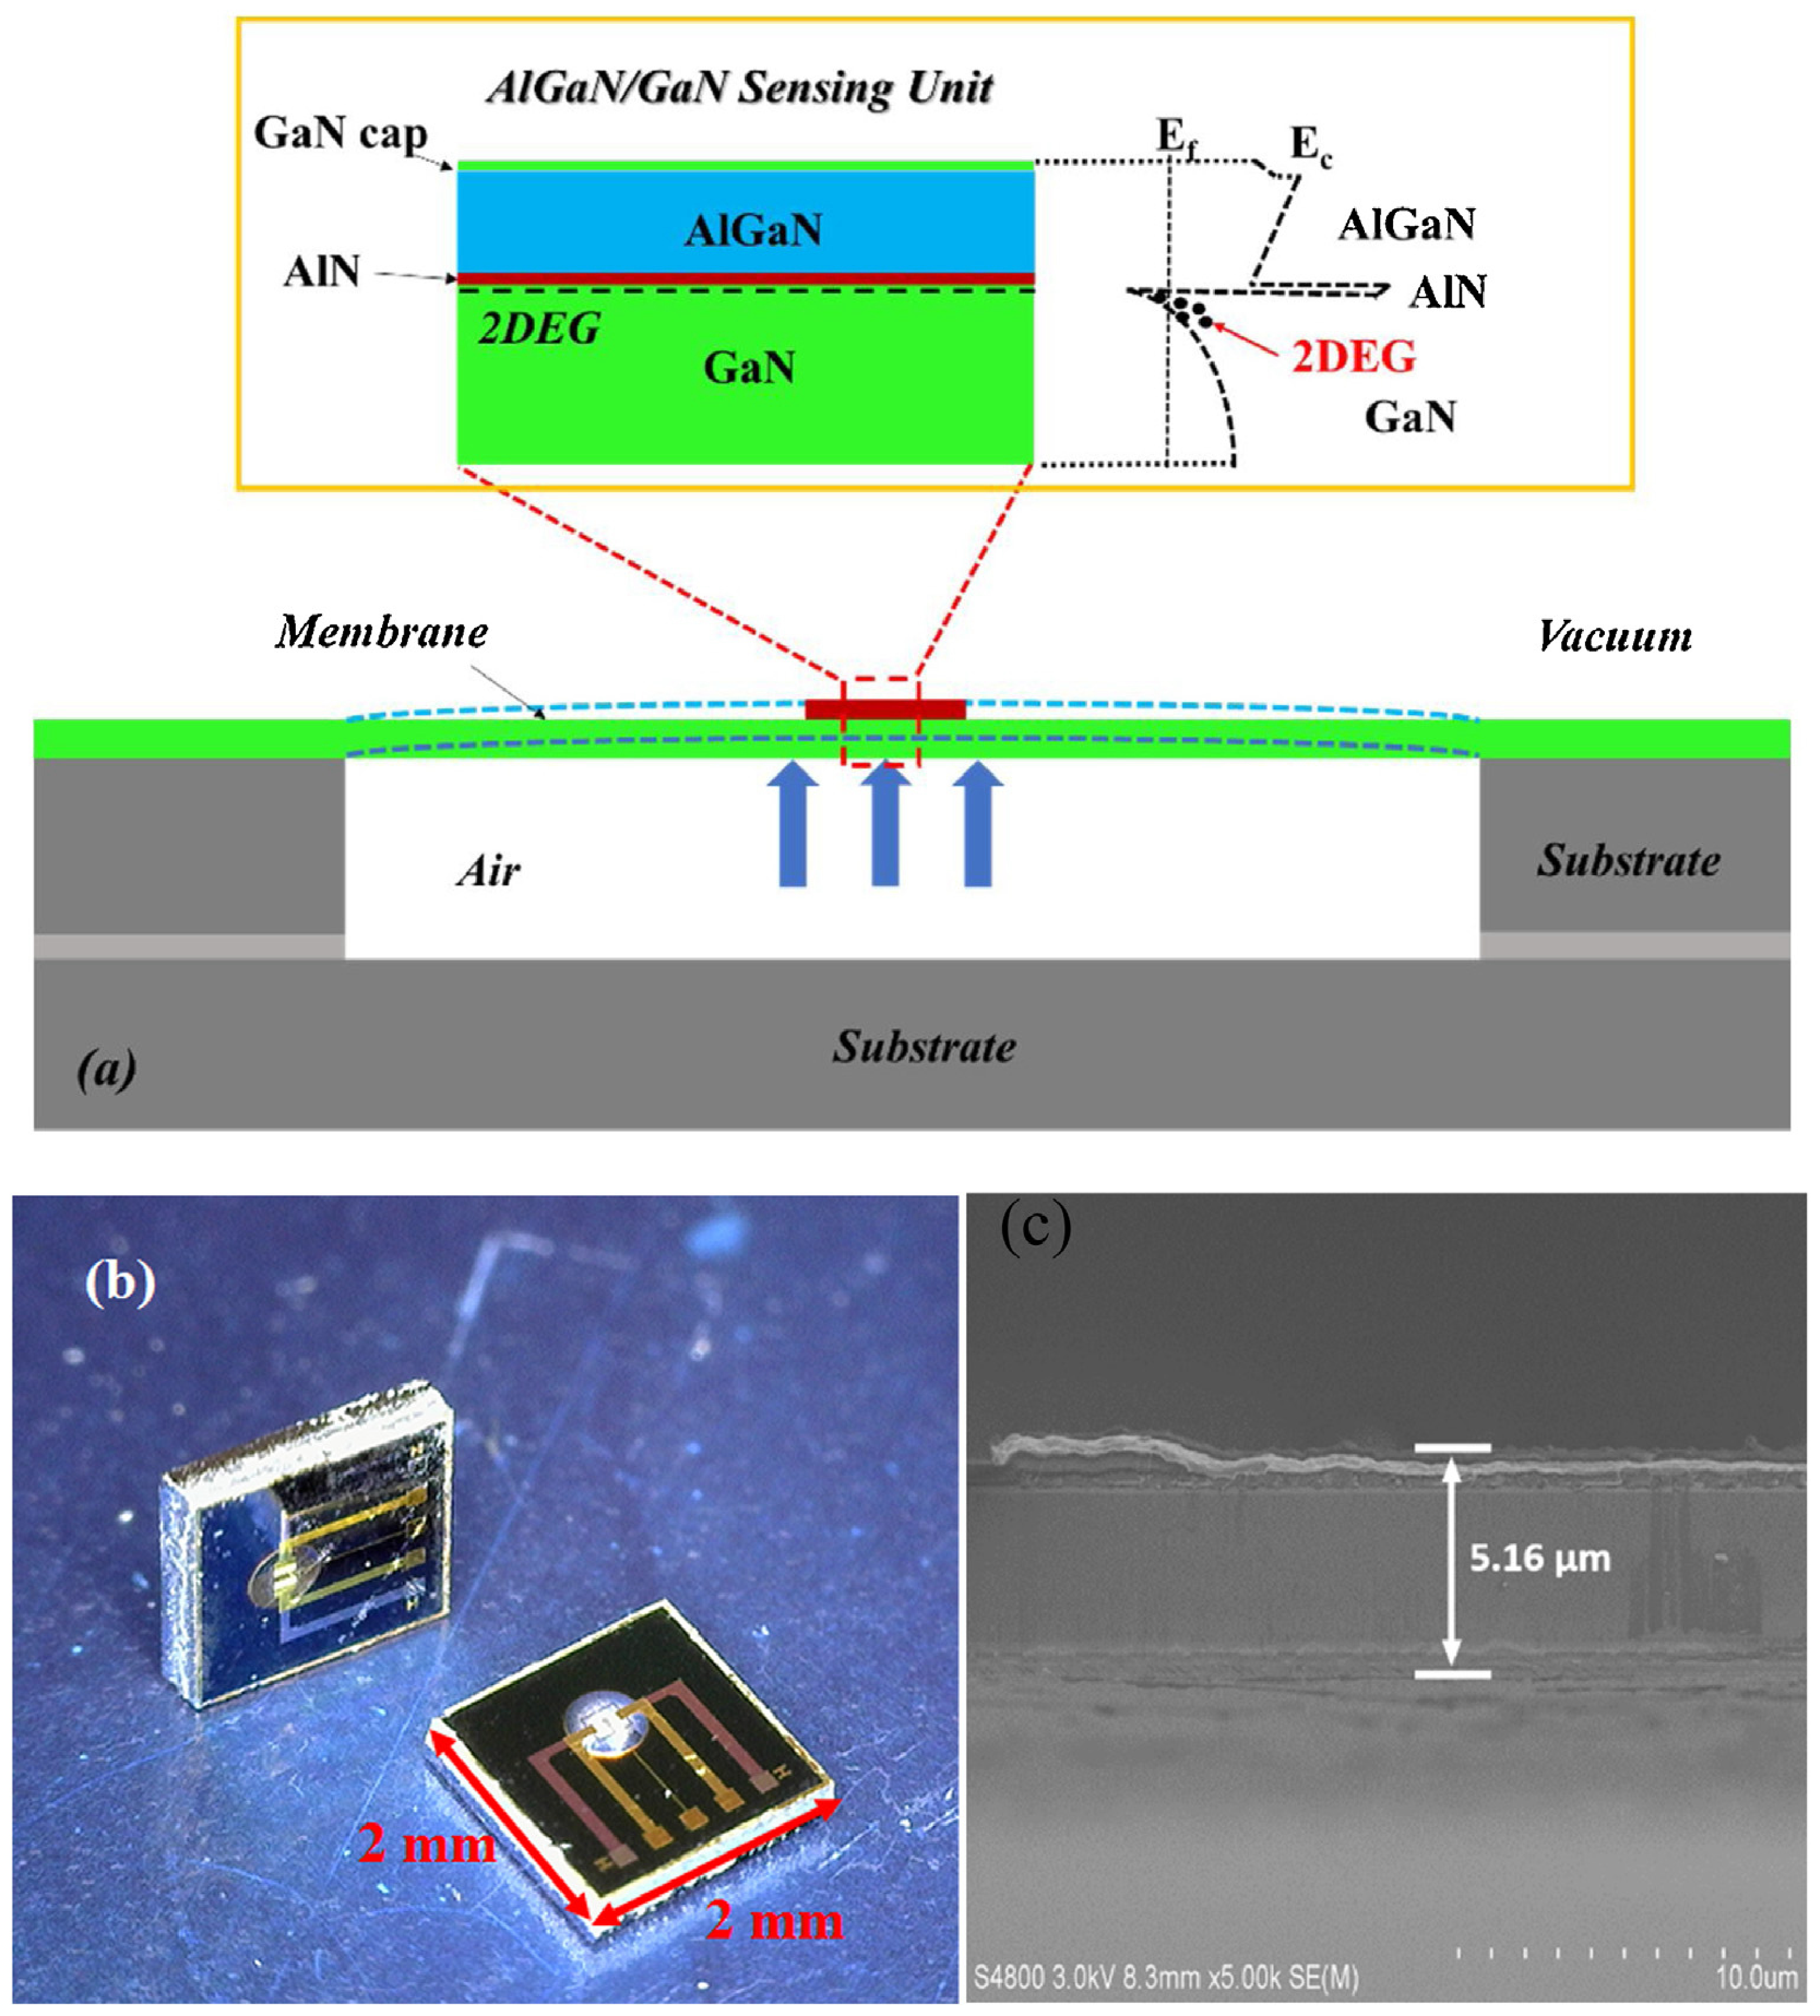
\includegraphics[width=0.9\textwidth]{ch1_16}
\caption[Miniature pressure MEMS sensor based on AlGaN/GaN heterojunction suspended structure]{Miniature pressure MEMS sensor based on AlGaN/GaN heterojunction suspended structure \protect\cite{sun2020low}}
\label{fig:1.16}
\end{figure}


III-V nitride \index{Nitride} MEMS \index{MEMS} devices are also widely used in the field of biosensing. Indu Sarangadharan et al. reported a highly sensitive AlGaN/GaN \index{HEMT} HEMT bioMEMS sensor for detecting cardiac troponin I (\autoref{fig:1.17}) \cite{sarangadharan2018high}. The unique double-layer gate-controlling mechanism overcomes the shortcomings of charge screening in conventional Si-based MEMS biosensors and enables detection of target proteins in physiological solutions without sample processing 


\begin{figure}[H] 
\centering    
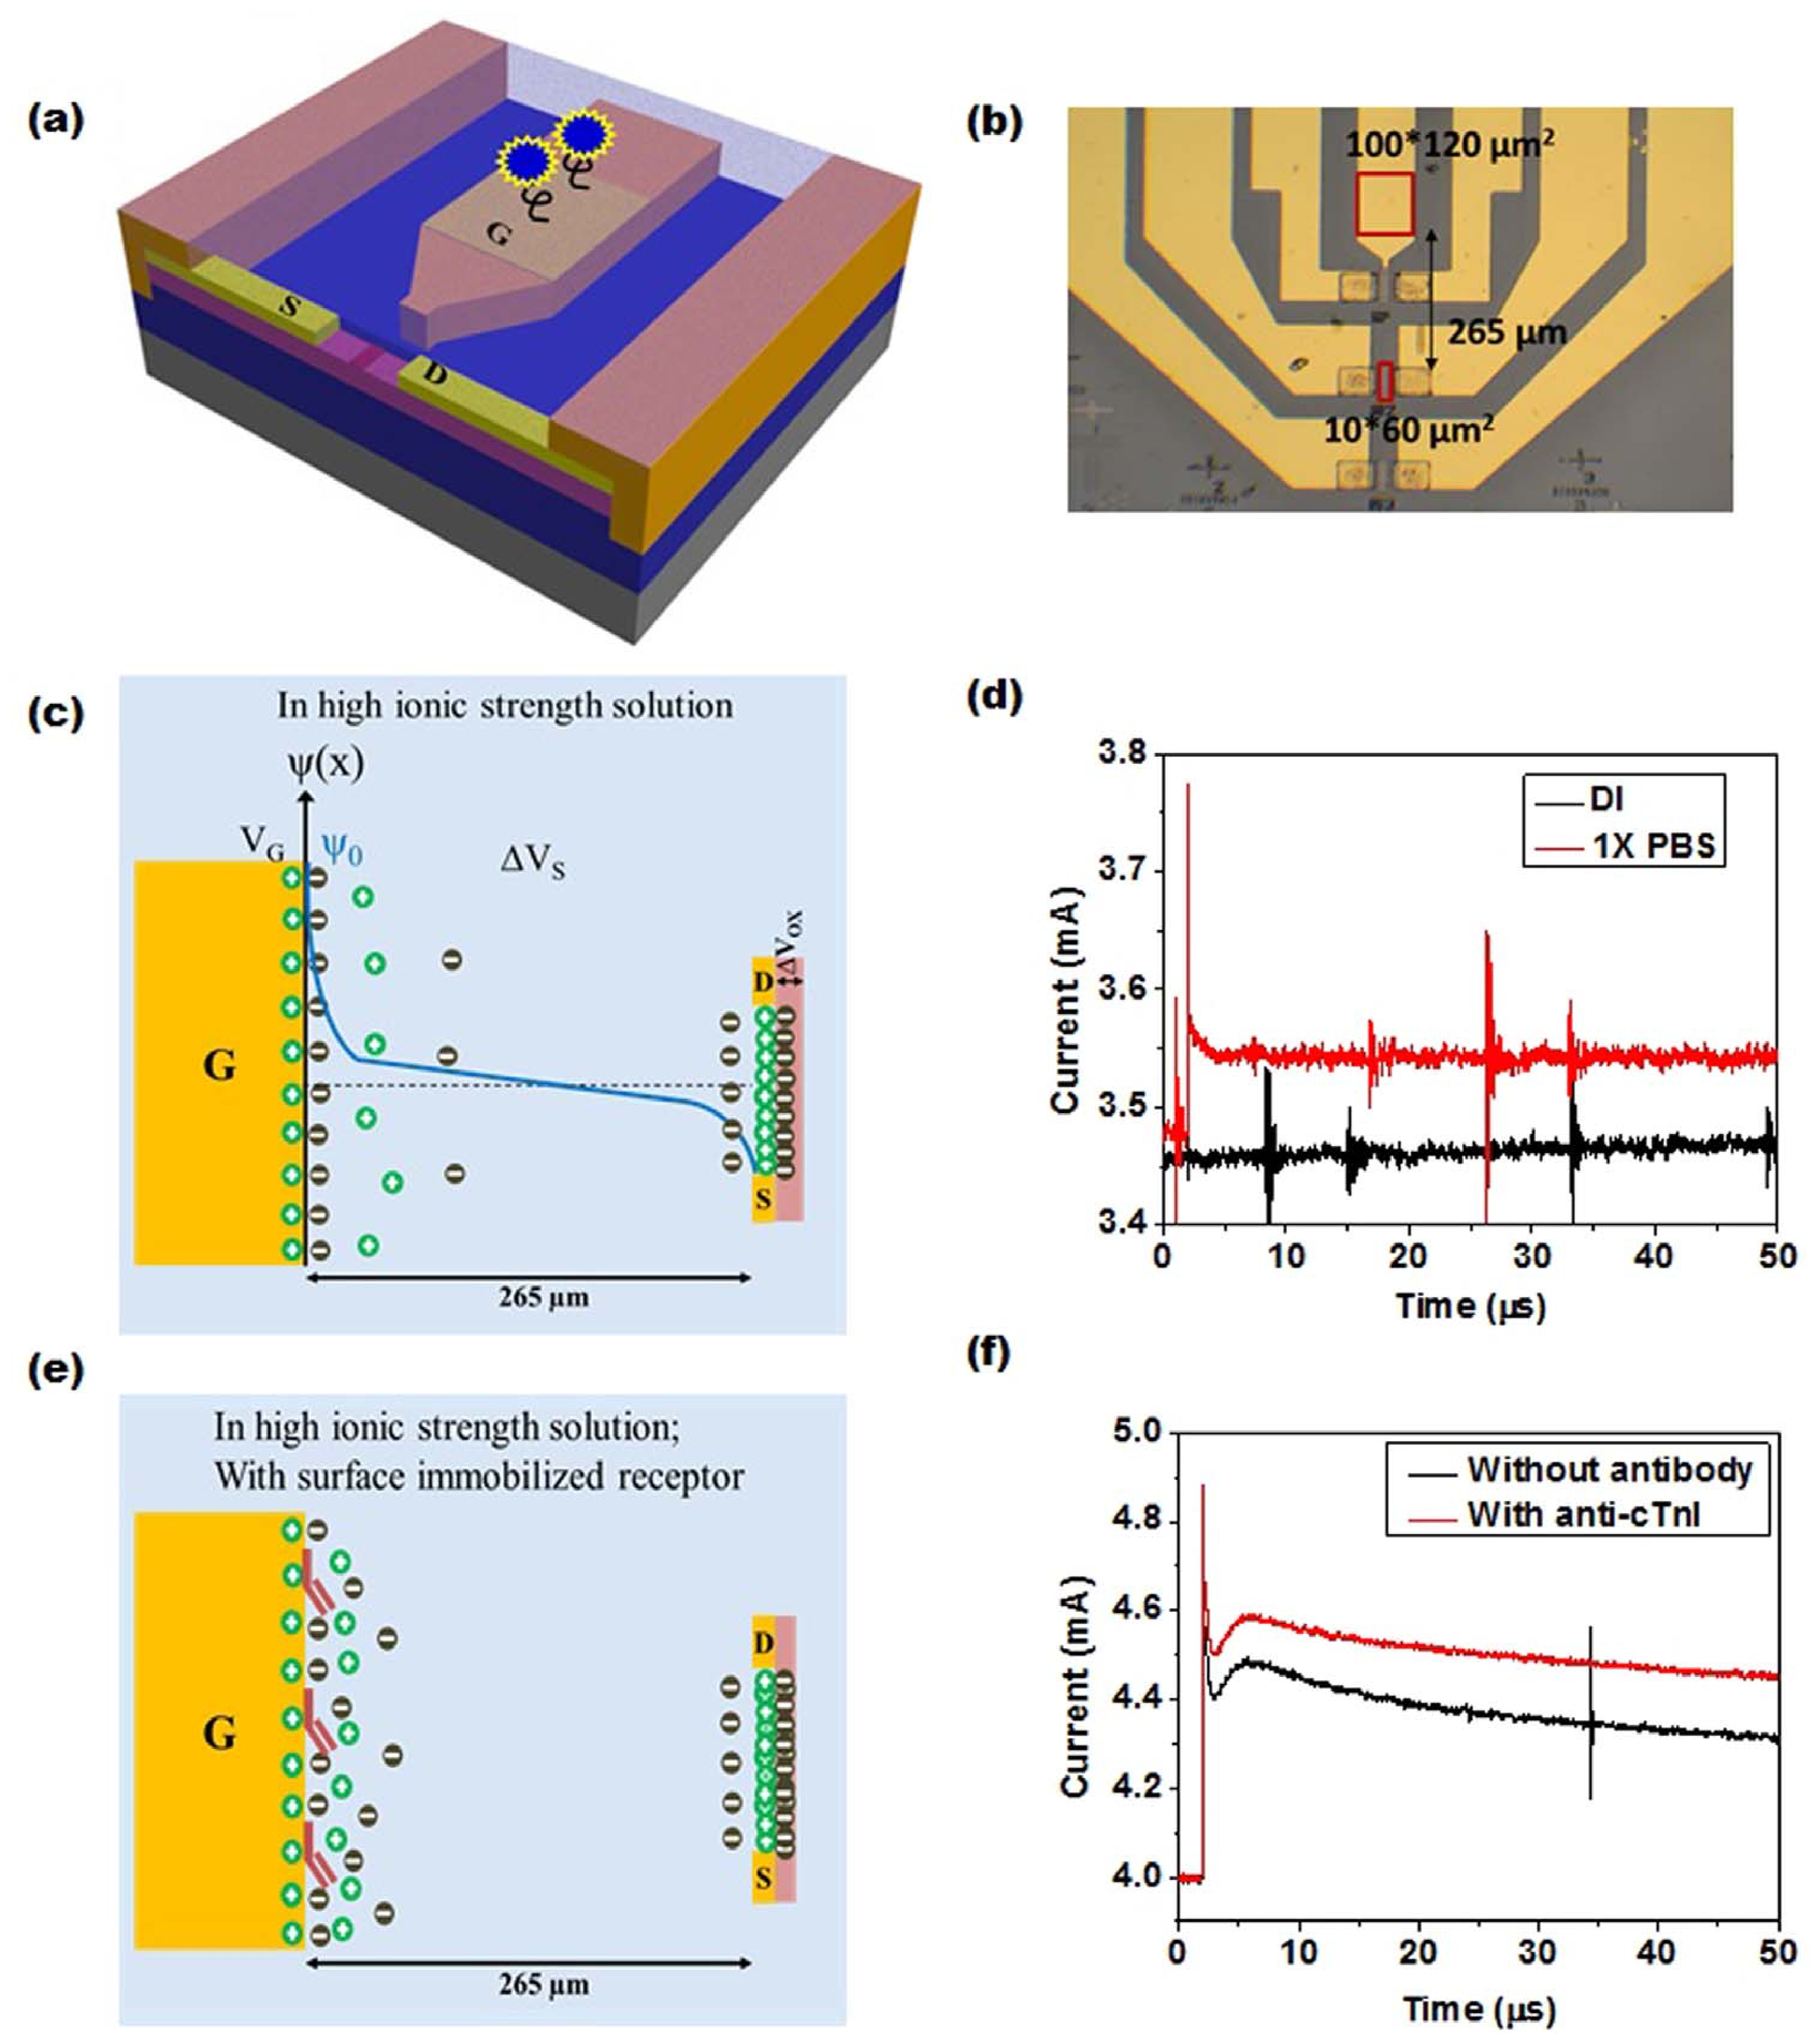
\includegraphics[width=0.9\textwidth]{ch1_17}
\caption[AlGaN/GaN HEMT MEMS biosensor for detecting cardiac troponin I in a physiological environment]{AlGaN/GaN HEMT MEMS biosensor for detecting cardiac troponin I in a physiological environment \protect\cite{sarangadharan2018high}}
\label{fig:1.17}
\end{figure}

\noindent steps, thus greatly simplifying the biosensor system. Tests using purified protein solutions and clinical serum samples showed that the sensor has high sensitivity, specificity, and a wide dynamic range (0.006 $\sim$ 148 \unit{ng/mL}) to quantitatively detect Calcin I in serum samples with sample volumes less than 2 \unit{uL} within 5 minutes. In addition, MEMS \index{MEMS} chips can be packaged in polymer substrates for easy integration with portable measurement units, which can serve as a fast, inexpensive, and highly sensitive cardiovascular disease detection device with broad applications in point-of-care diagnostics and personal healthcare systems.

\subsection{Microstructure of III-V nitrides}

With the deepening of the research on the properties of wide-bandgap semiconductor materials, the preparation technology of III-V \index{Nitride} nitrides has made significant progress. More complex MEMS \index{MEMS} devices structures can be prepared by heterojunction epitaxial \index{Epitaxial!growth} growth, thin film \index{Thin film} deposition (epitaxial film and polycrystalline film), inductively coupled plasma (ICP) \index{Inductively coupled plasma (ICP)} etching process, and photoelectrochemical (PEC) etching process \cite{strittmatter2004development,zorman2008micro,brueckner2011micro,yamada2021fabrication,davies2004fabrication,lv2011characterization-a,lv2011characterization-b}.

\begin{figure}[H] 
\centering    
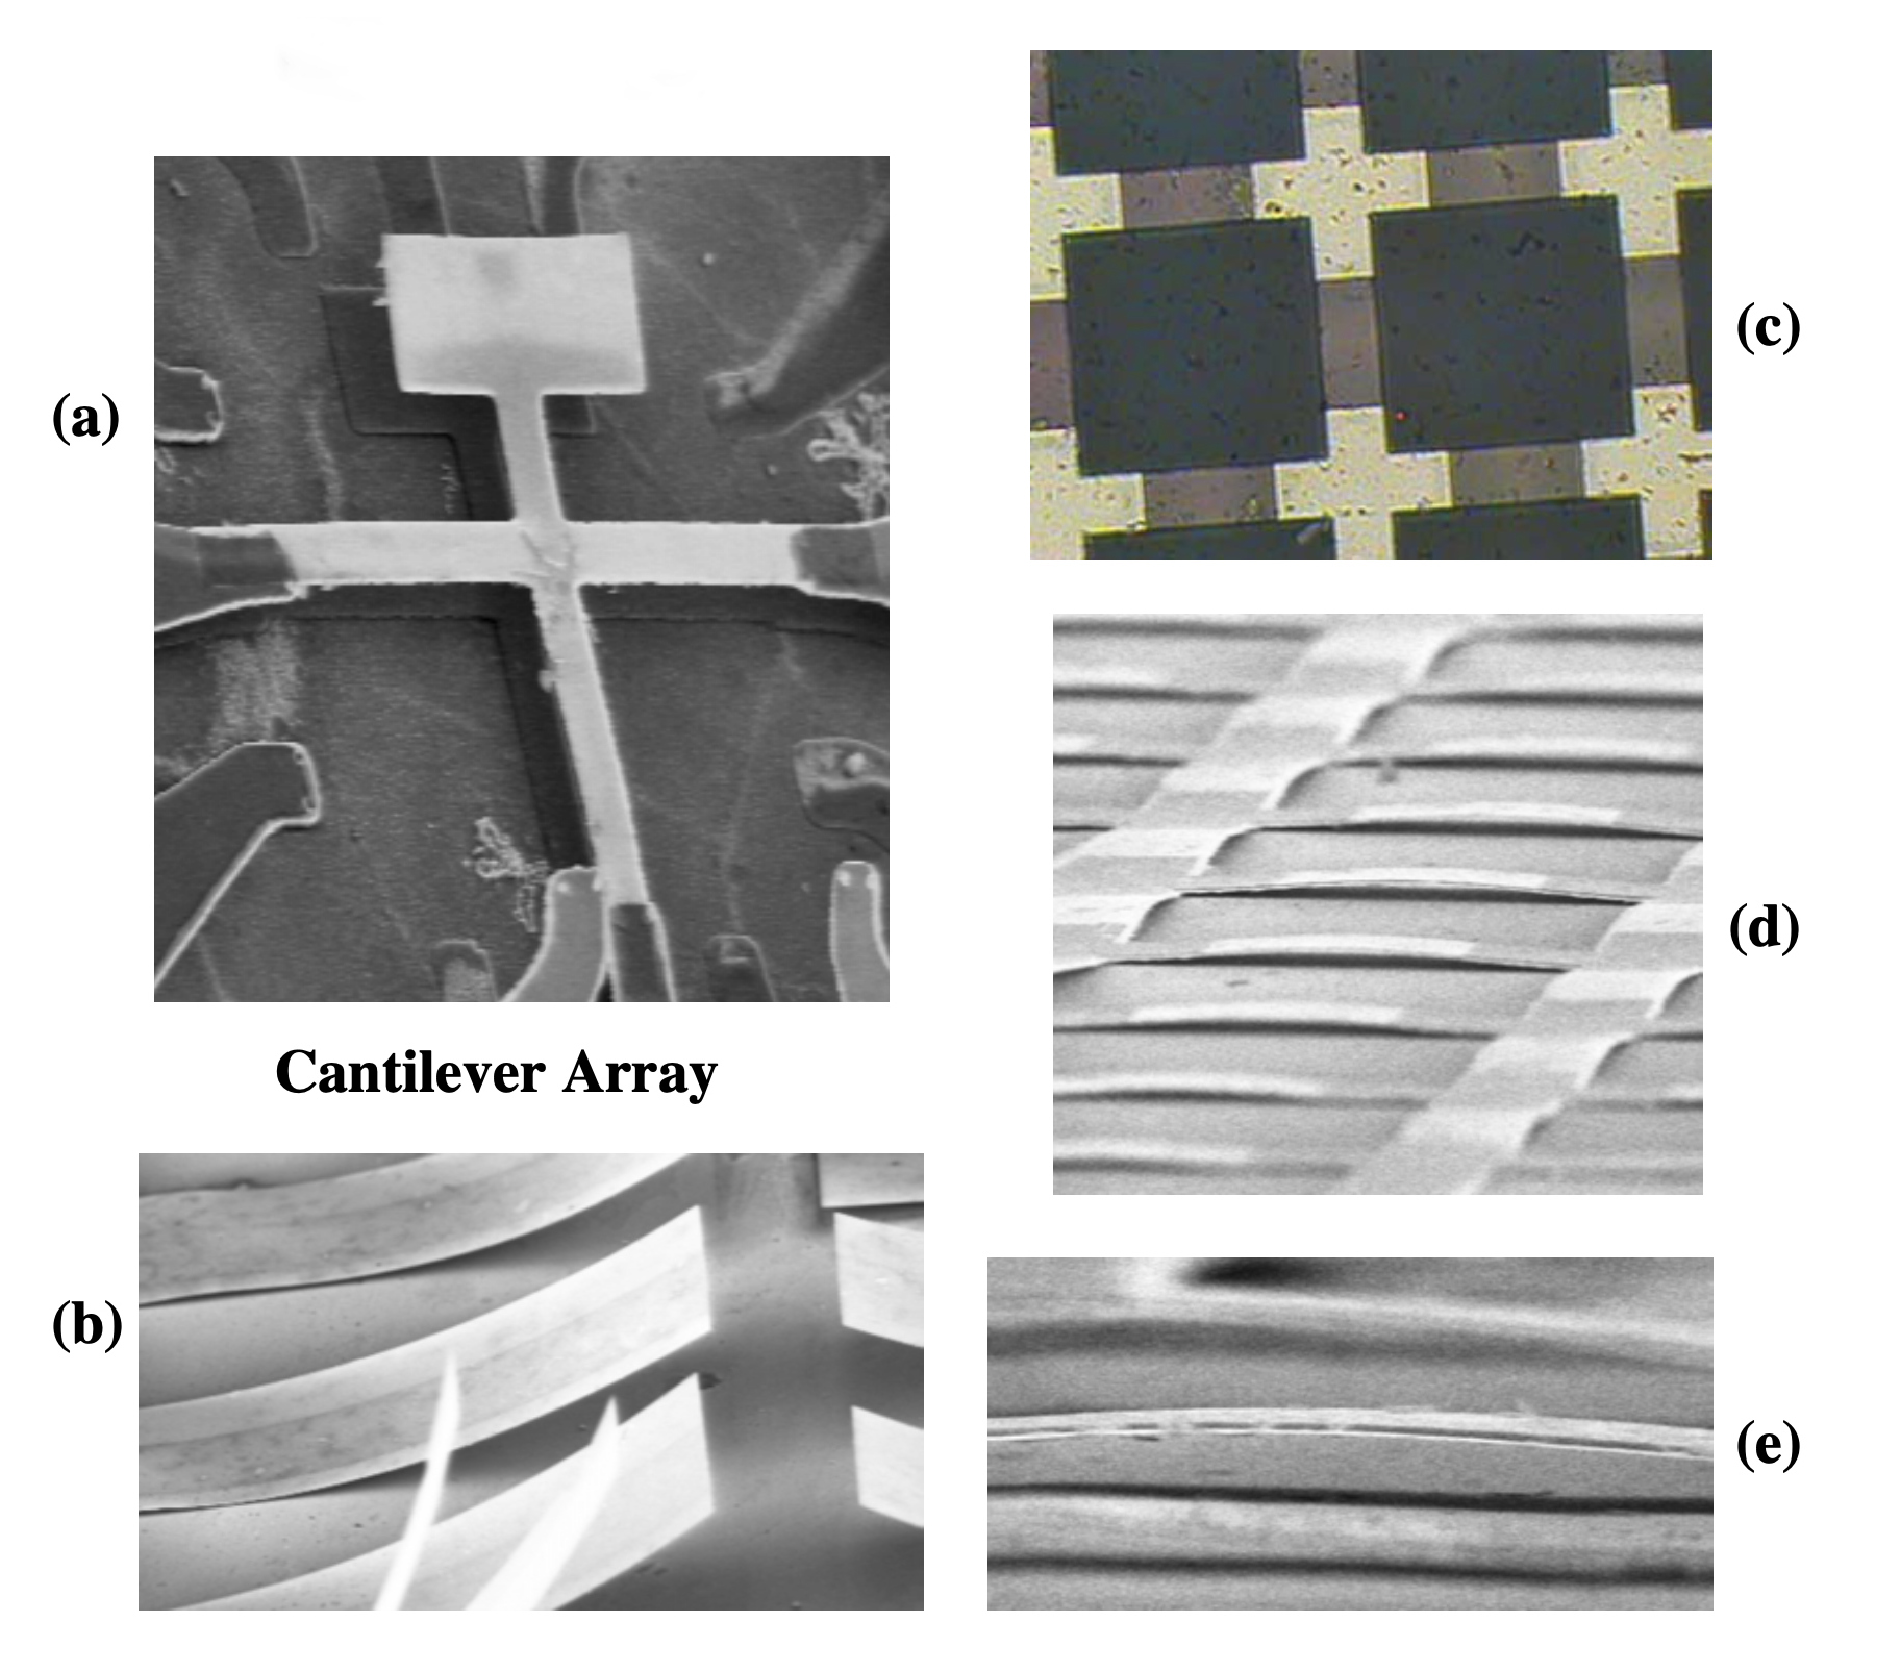
\includegraphics[width=0.9\textwidth]{ch1_18}
\caption[SEM image of a series of p-GaN microcantilever arrays]{SEM image of a series of p-GaN microcantilever arrays \protect\cite{strittmatter2004development}}
\label{fig:1.18}
\end{figure}

\begin{figure}[H] 
\centering    
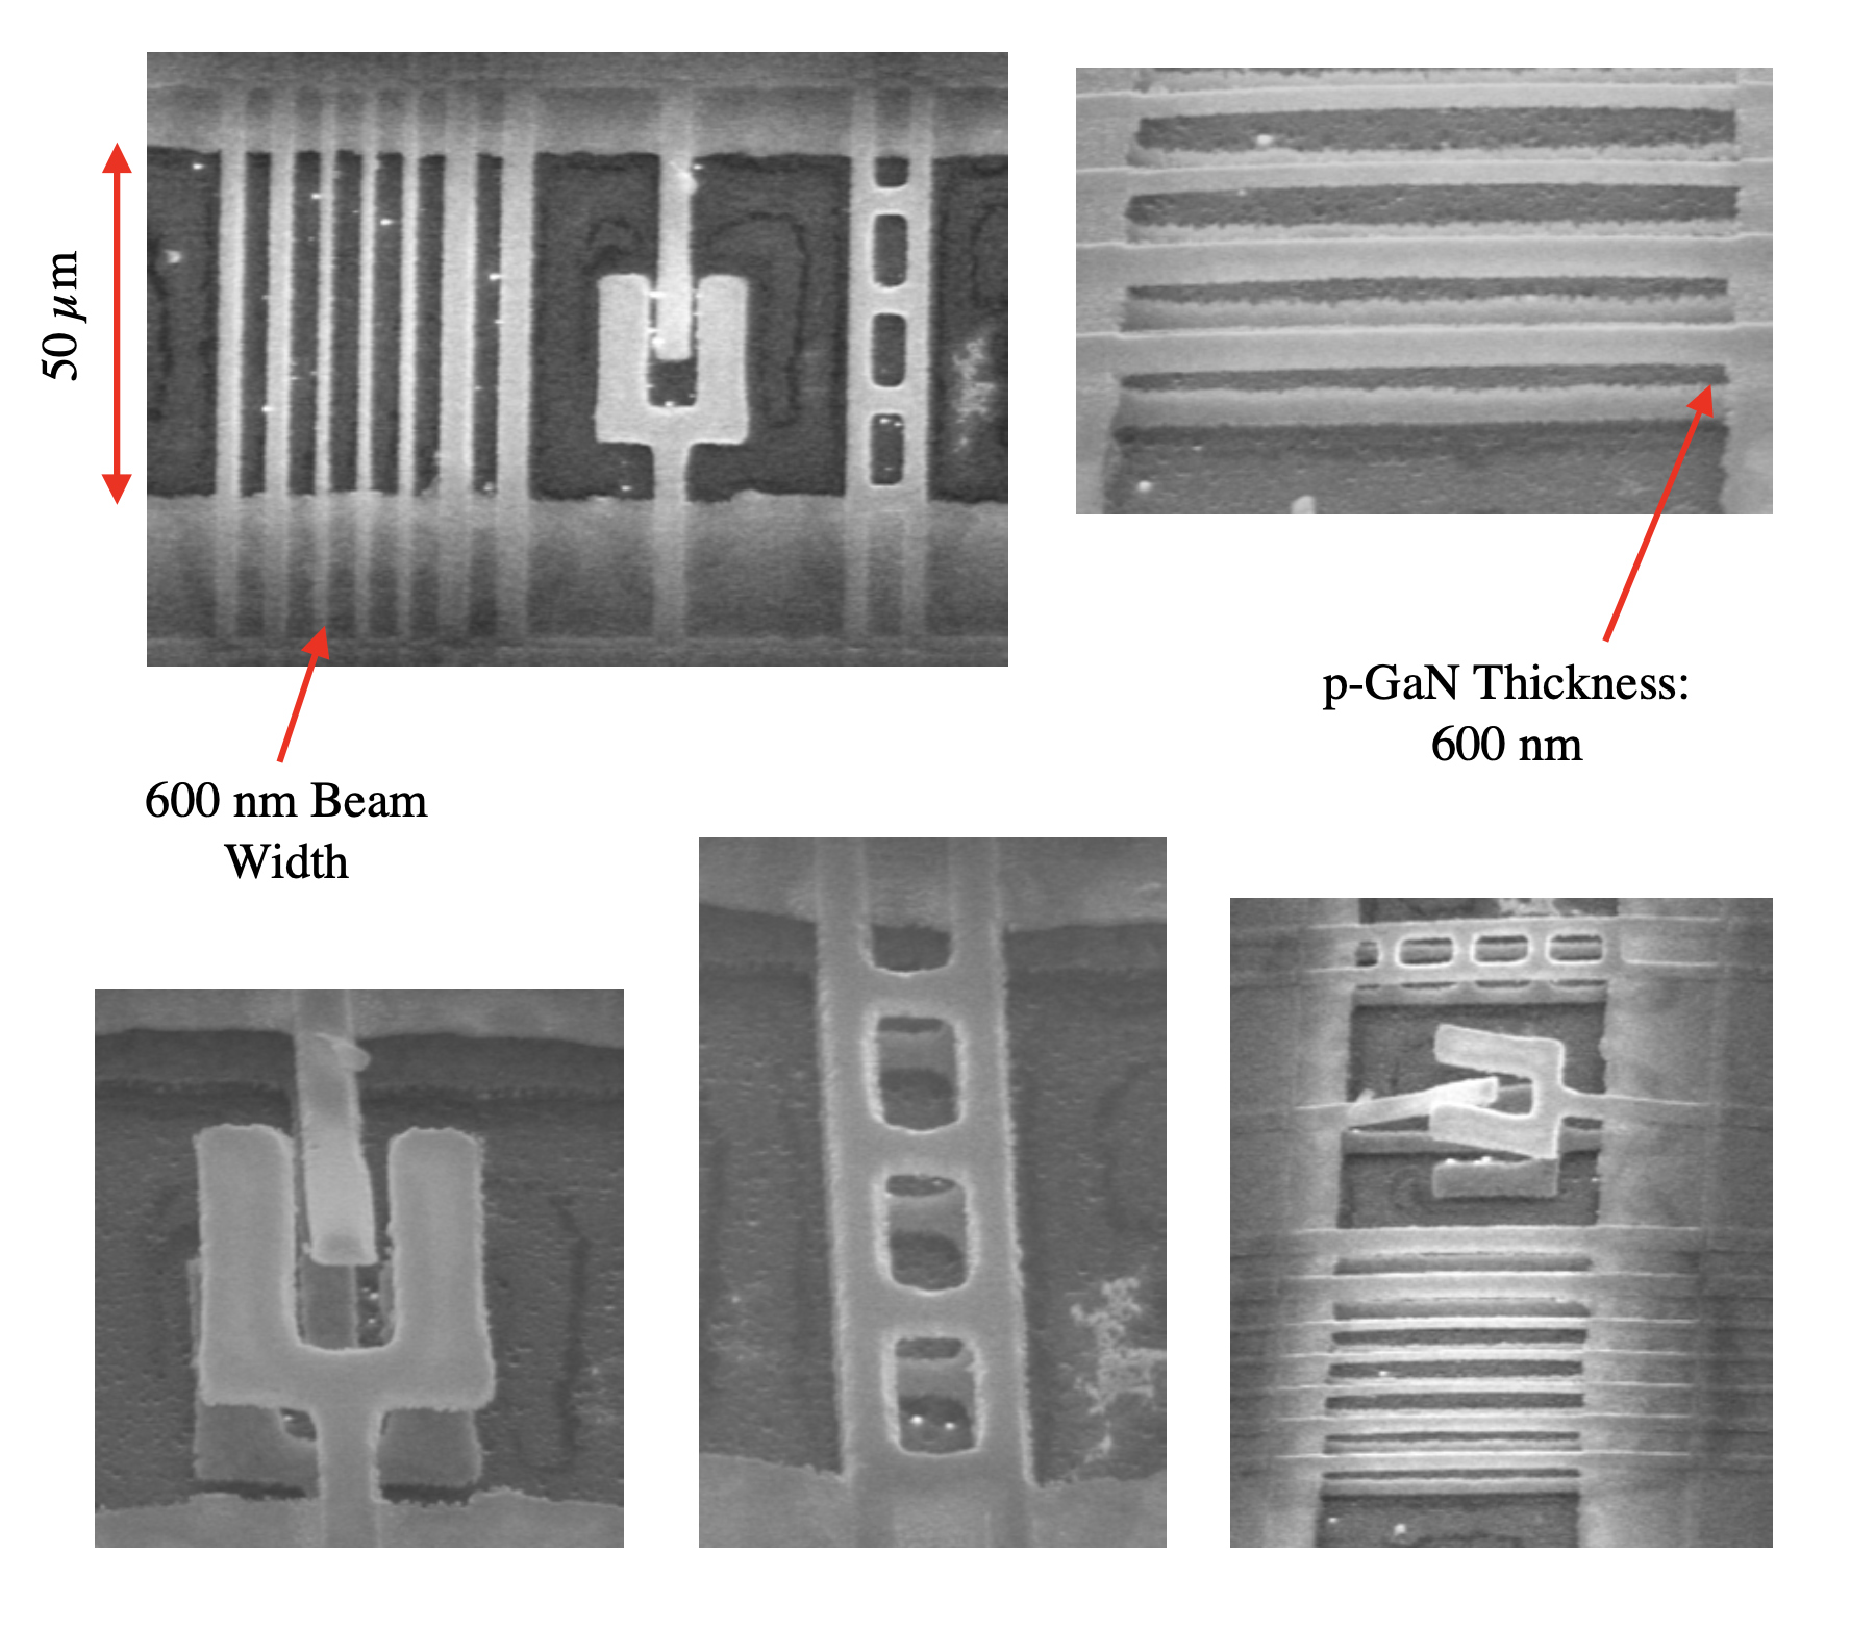
\includegraphics[width=0.9\textwidth]{ch1_19}
\caption[SEM image of a series of p-GaN structures suspended between two half-plane supports]{SEM image of a series of p-GaN structures suspended between two half-plane supports \protect\cite{strittmatter2004development}}
\label{fig:1.19}
\end{figure}

\autoref{fig:1.18} shows a series of p-GaN microcantilever arrays fabricated by a PEC etch process. The etched p-GaN cantilever \index{Cantilever} relaxes into a uniformly curved shape along the direction away from the \index{Substrate} substrate. This is because a vertical stress gradient is introduced in the p-GaN layer due to crystal \index{Crystal} defects during the growth process \cite{strittmatter2004development}. \autoref{fig:1.19} shows a series of p-GaN structures suspended between two half-support planes fabricated by the PEC process, with a lateral dimension of about 1 \unit{\um} and a minimum beam width of only 600 \unit{\nm}. The lateral dimension of the device reaches the sub-micron scale, which indicates that GaN-based MEMS devices can be easily extended to the field of nano-electromechanical systems (NEMS). Advances in III-V nitride \index{Nitride} preparation technology have greatly promoted the development of new III-V nitride power MEMS \index{MEMS} devices.

\section{Outline of the thesis} 

\noindent This thesis systematically studies the theoretical modeling and device fabrication of III-V nitride power MEMS based on the cantilever \index{Cantilever} structure of \index{AlGaN/AlN/GaN heterojunction} AlGaN/AlN/GaN heterojunction. \autoref{fig:1.20} illustrates the structure and SEM \index{Scanning electron microscopy (SEM)} image of GaN power MEMS devices. The active area \index{Active region} is at the junction of the cantilever and the \index{Wafer} wafer, which is enlarged in the figure. Due to the design of cantilever \index{Cantilever} structure, the external stimulus from direct \index{Strain} strains or non-contact magnetic force \index{Magnetic!force} will be greatly amplified, thereby introducing the piezoelectric polarization charges \index{Piezoelectric!polarization charge} in the active \index{Active region} area. Based on the piezotronics \index{Piezotronics} effect, the piezoelectric polarization charges generated by external stimulus can modulate the energy band at the AlGaN/AlN/GaN heterojunction, thereby effectively adjusting the 2DEG concentration \index{Two-dimensional electron gas (2DEG)} and finally controlling the output current \index{Output!current} and power density of the MEMS devices.

\begin{figure}[H] 
\centering    
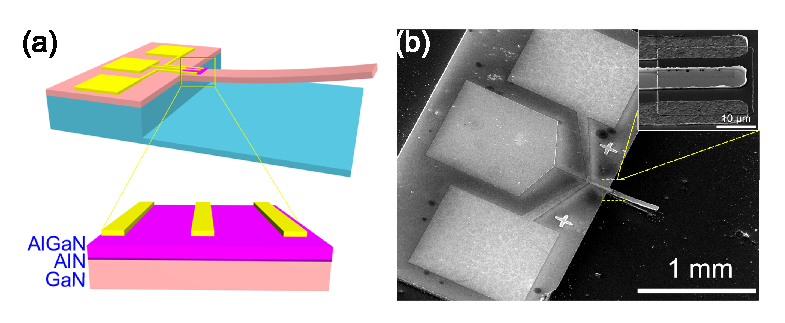
\includegraphics[width=0.9\textwidth]{ch1_20}
\caption[Structure and SEM image of GaN power MEMS devices]{Structure and SEM image of GaN power MEMS devices}
\label{fig:1.20}
\end{figure}

The physical framework \index{Physical!framework} and mathematical analysis method are presented to model the modulation \index{Modulation} characteristics of the external stress on the energy band \index{Energy band} of the \index{AlGaN/AlN/GaN heterojunction} AlGaN/AlN/GaN heterojunction and the electrical properties of the MEMS \index{MEMS} device, which provide theoretical guidance for the design of III-V nitride \index{Nitride} power MEMS. On this basis, two types of novel power MEMS \index{MEMS} devices based on the cantilever \index{Cantilever} structure of \index{AlGaN/AlN/GaN heterojunction} AlGaN/AlN/GaN heterojunctions were designed and fabricated, namely, a strain-controlled power MEMS devices (SPD) \index{Strain-controlled power MEMS devices (SPD)} and a \index{Magnetosensory power MEMS devices (MPD)} magnetic field-controlled power MEMS devices (MPD), in which external strain \index{Strain} and magnetic field \index{Magnetic!field} can significantly modulate \index{Modulation} the output power \index{Output!power} density of MEMS \index{MEMS} devices due to the micro-cantilever \index{Cantilever} structure.\\

\begin{figure}[H] 
\centering    
\includegraphics[width=0.9\textwidth]{Outline}
\caption[The outline of the thesis]{The outline of the thesis}
\label{fig:outline}
\end{figure}

\noindent The content of this thesis is mainly composed of the following three parts: \\

\begin{large}
\centerline{Part \uppercase\expandafter{\romannumeral1} \quad Theory}
\end{large}

~\\

\noindent Chapter 2. Theoretical model of MEMS cantilever devices\\

\noindent In this study, a semi-classical physical model of the MEMS \index{MEMS} device with a cantilever \index{Cantilever} structure based on \index{AlGaN/AlN/GaN heterojunction} AlGaN/AlN/GaN heterojunction was established using piezotronics \index{Piezotronics} theory. The mathematical relationship between the lattice strain \index{Lattice!strain} of the thin film \index{Thin film} and the piezoelectric polarization charge intensity \index{Piezoelectric!polarization charge} in the multilayer heterojunction was deduced through piezoelectric constitutive equation \index{Piezoelectric!constitutive equation} and biaxial stress \index{Biaxial stress model} model. The finite element analysis \index{Finite element analysis} method of material mechanics is used to calculate the piezoelectric polarization charge intensity of the heterojunction film under different external stresses, and then the self-consistent coupling computational model \index{Self-consistent computational model} of the one-dimensional Schrödinger-Poisson coupling equation \index{Schrödinger-Poisson coupling equation} was used to calculate the modulation \index{Modulation} characteristics of the external stress on the \index{Two-dimensional electron gas (2DEG)} 2DEG concentration and energy band \index{Energy band} of the AlGaN/AlN/GaN heterojunction, as well as the electrical properties of the MEMS device. Based on the theoretical model, the new AlGaN/AlN/GaN power MEMS have been designed and fabricated, namely \index{Strain-controlled power MEMS devices (SPD)} SPD and \index{Magnetosensory power MEMS devices (MPD)} MPD. This study provides theoretical guidance for the development of new MEMS cantilever \index{Cantilever} devices based on AlGaN/AlN/GaN heterojunctions.\\

\begin{large}
\centerline{Part \uppercase\expandafter{\romannumeral2} \quad Manufacturing}
\end{large}

~\\

\noindent Chapter 3. Manufacturing Technology of Power MEMS Devices\\

\noindent In the Part II, the manufacture of GaN power MEMS devices from epitaxial growth \index{Epitaxial!growth} wafers \index{Wafer} to well-functional devices will be systematically studied. Benefiting from the rapid development of III-V compound semiconductor fabrication and characterization equipment, various complex microstructures including GaN microcantilever \index{Cantilever} structures can now be easily realized by equipment with different functions. This chapter introduced the main nanofabrication and characterization equipment, including epitaxial \index{Epitaxial!growth} growth, dry \index{Etching!dry etching} etching, photolithograph\index{Photolithography}y, thin film \index{Thin film} deposition, plasma \index{Cleaning!plasma cleaning} cleaning, Raman \index{Raman!spectroscopy} spectroscopy, scanning \index{Scanning electron microscopy (SEM)} electron microscopy, transmission \index{Transmission electron microscopy (TEM)} electron microscopy, etc. I briefly introduced their important role in GaN power MEMS \index{MEMS} research, as well as the corresponding process \index{Fabrication process} design and key parameters.\\

\noindent Chapter 4. Process Development and Integration of Power MEMS Devices\\

\noindent In this chapter, I developed the corresponding process parameters and their process integration based on the manufacturing technology and equipment, thus realizing the whole process from GaN wafer \index{Wafer} to device. The processes in this chapter have been described in detail about the main purpose of the process, the equipment used, and the detailed recipe parameters. Moreover, in order to visualize the fabrication \index{Fabrication process} process flow, a corresponding flow chart has been drawn to illustrate the main process steps. Step by step, high-performance GaN \index{HEMT} HEMTs and GaN power \index{MEMS} MEMS devices have been successfully fabricated.\\

\begin{large}
\centerline{Part \uppercase\expandafter{\romannumeral3} \quad Devices}
\end{large}

~\\

\noindent Chapter 5. Strain-controlled power MEMS devices\\

\noindent In this study, we designed a strain \index{Strain} modulated \index{Modulation} power MEMS device \index{Strain-controlled power MEMS devices (SPD)} (Strain-controlled Power Device, SPD) based on the cantilever structure \index{Cantilever} of \index{AlGaN/AlN/GaN heterojunction} AlGaN/AlN/GaN heterojunction, which uses external strain \index{Strain} to directly modulate \index{Modulation} the output power \index{Output!power} of the device by simulating the reflection process of the human reflex. Based on the piezotronics \index{Piezotronics} effect, the piezoelectric polarization charges \index{Piezoelectric!polarization charge} generated by external strain can modulate the energy band \index{Energy band} at the AlGaN/AlN/GaN heterojunction, thereby effectively adjusting the \index{Two-dimensional electron gas (2DEG)} 2DEG concentration, and finally controlling the output current \index{Output!current} and power density of the SPD. At the same time, similar to the ultimate control ability of the brain in the knee-jerk reflex mechanism, the gate voltage \index{Voltage!gate voltage} of the SPD \index{Strain-controlled power MEMS devices (SPD)} can control the output power \index{Output!power} in a wider range, thus combining the dimensional control advantage of both small-scale external strain \index{Strain} control and large-scale programmable gate voltage \index{Voltage!gate voltage} control, which means that the strain \index{Strain} modulation \index{Modulation} power is programmable. This study not only provides new insights into the interplay of mechanical stimulation and power control, but could also lead to the development of biomimetic smart powered devices that resemble human reflexes.\\

\noindent Chapter 6. Magnetosensory power MEMS devices.\\

\noindent In this study, we fabricated a \index{Magnetic!field} magnetic field-regulated power MEMS device (Magnetosensory Power Devices, MPD) \index{Magnetosensory power MEMS devices (MPD)} by depositing a magnetic thin film \index{Magnetic!thin film} on the front end of a cantilevered \index{Cantilever} GaN HEMT \index{HEMT} based on \index{AlGaN/AlN/GaN heterojunction} AlGaN/AlN/GaN heterojunction, which can directly control the output power \index{Output!power} through an external magnetic field. Moreover, the output power of the MPD has a linear relationship with the external magnetic field, showing good magnetic regulation characteristics. Based on the piezotronics \index{Piezotronics} effect, the magnetic force \index{Magnetic!force} generated by the external magnetic field can generate corresponding piezoelectric polarization charges \index{Piezoelectric!polarization charge} at the interface \index{Interface} of the \index{Thin film} thin film, which can modulate \index{Modulation} the energy band \index{Energy band} of the AlGaN/AlN/GaN heterojunction, thereby effectively adjusting the 2DEG \index{Two-dimensional electron gas (2DEG)} concentration, and finally controlling the output power \index{Output!power} of the MPD. At the same time, similar to the bio-voltage signal between neuron synapses which effectively regulated the magnitude of neuronal signal in a larger range, the output power is controlled at a larger range by the gate voltage \index{Voltage!gate voltage} of MPD. Therefore it combines the two-dimensional control advantage. This work not only provides physical electronics insights into the working mechanism of magnetic sensing neurons in the biological sense, but also can promote the development of various neuroelectronic devices.\\
